\documentclass[12pt, a4paper]{article}
\usepackage[utf8]{inputenc}
\usepackage{comment, listings, centernot, amssymb, hyperref, graphicx, amsmath, textcomp, breqn, mathtools, csquotes, cancel, enumitem, amsthm, caption, bm, tikz} % amsthm provides `proof`environment
\usepackage[backend=biber]{biblatex}
\usepackage[english]{babel}
\usepackage{mathrsfs}
\usepackage{array}
\usepackage{cancel}
\addbibresource{references.bib}

% NEW (16-04-21, 19p49)
\usepackage[margin = 1in]{geometry}
\numberwithin{equation}{section}

\theoremstyle{definition}
\newtheorem{thm}{Theorem}[section] % reset theorem numbering for each chapter

\theoremstyle{definition}
\newtheorem{defn}[thm]{Definition} % definition numbers are dependent on theorem numbers
\newtheorem{exmp}[thm]{Example} % same for example numbers
\newtheorem{lemma}[thm]{Lemma} % same for example numbers
\newtheorem{remark}[thm]{Remark} % same for example numbers
\newtheorem{theorem}[thm]{Theorem} 
\newtheorem{corollary}[thm]{Corollary}
\newtheorem{proposition}[thm]{Proposition}
\newcommand{\norm}[2]{\left\vert\left\vert #1 \right\vert\right\vert_{#2}}
\newcommand{\abs}[1]{\left\vert #1 \right\vert}
\newcommand{\inner}[1]{\left\langle #1 \right\rangle}
\newcommand{\epi}[1]{\text{epi($ #1 $) } }
\newcommand{\floor}[1]{\lfloor #1 \rfloor}
\newcommand{\seq}[1][\varphi]{\left( #1 \right)_{n \in \mathbb{N}}}
\renewcommand{\qedsymbol}{$\blacksquare$}

\title{Mathematics}
% \subtitle{Questions}
\author{Imahn Shekhzadeh}
\date{\today}

% https://tex.stackexchange.com/a/94397/239562
\binoppenalty=10000 
\relpenalty=10000 

% https://tex.stackexchange.com/a/9110/239562
\emergencystretch 3em



\begin{document}
	\maketitle
	\tableofcontents
	\newpage 
	
	\section{Algebra}
	
	\begin{defn}[Action]\label{defn:algebra__group_action}
		Let $G$ be a group (where $e$ is the neutral element), and $X$ a set. Then a (left) group action $\alpha$ of $G$ on $X$ is a function
		\begin{align}
			\alpha: G\times X \rightarrow X
		\end{align}
		satisfying the following two axioms $(\forall g, h\in G) \wedge (\forall x\in X)$:
		\begin{align*}
			\alpha(e, x) &= x, 
			\\ \alpha(g, \alpha(h, x)) &= \alpha(gh, x)
		\end{align*}
		The group action is commonly written as $g\cdot x$ s.t.~the axioms become
		\begin{align}\label{eqn:left__group_action}
			e\cdot x &= x, 
			\\ g\cdot \left(h\cdot x\right) &= \left(gh\right)\cdot x
		\end{align}
		A right group action of $G$ on $X$ is a function
		\begin{align}
			\alpha: X\times G \rightarrow X
		\end{align}
		satisfying the following two axioms $(\forall g, h\in G) \wedge (\forall x\in X)$:
		\begin{align}
			\alpha(x, e) &= x, 
			\\ \alpha(\alpha(x, g), h) &= \alpha(x, gh)
		\end{align}
	\end{defn}
	
	\begin{exmp}
		Consider $G = \text{SO}(2)$, i.e.~the group of all rotations in $\mathbb R^2$, with the group operation given by the composition of rotations, and let $X = S^1$ be the unit circle in $\mathbb C$. Now consider the group action
		\begin{align}
			\Phi:\text{SO}(2) \times S^{1} \rightarrow S^{1}, (R_{\theta}, p) \mapsto R_{\theta}(p)
		\end{align}
		This is a group action on $X = S^{1}$, since 
		\begin{align*}
			\Phi(R_{\theta_1}, \Phi(R_{\theta_2}, p)) = \Phi(R_{\theta_1 + \theta_2}, p).
		\end{align*}
		In the short notation, one would write this as
		\begin{align*}
			R_{\theta_1}\cdot \left( R_{\theta_2} \cdot p \right) = R_{\theta_1 + \theta_2} \cdot p.
		\end{align*}
	\end{exmp}
	
	\begin{defn}[Signals\footnote{\cite[p.~11]{bronstein2021geometric}}] 
		Let $V$ be a vector space\footnote{In computer vision, its dimensions would be called \textit{channels}.} and $\Omega$ a set, possibly with additional structure. Then the space of $V$-valued signals on $\Omega$,
		\begin{align}
			\mathcal X(\Omega, V) = \{ x: \Omega \rightarrow V \}
		\end{align}
		is a function space with a vector space structure. (Note that each $x\in \mathcal X(\Omega, V)$ is a signal.)
		
		Addition and scalar multiplication of signals are defined as 
		\begin{align}
			(\alpha x + \beta y)(u) := \alpha x(u) + \beta y(u) \quad \forall u\in\Omega\ \forall \alpha, \beta\in \mathbb R.
		\end{align}
	\end{defn}

	\begin{lemma}
		If $V$ is endowed with an inner product $\langle v, w\rangle_{V}$ and a measure $\mu$ on a $\sigma$-algebra defined on the set $\Omega$ (wrt which an integral can be defined), we have the following induced inner product on $\mathcal X(\Omega, V)$
		\begin{align}
			\langle x, y\rangle_{\mathcal X(\Omega, V)} := \int_{\Omega}\langle \underbrace{x(u)}_{\in V}, \underbrace{y(u)}_{\in V}\rangle_{V}d\mu(u)
		\end{align}
	\end{lemma}

	\begin{proof}
		Trivial.
	\end{proof}

	\begin{remark}
		The domain (set) $\Omega$ can be discrete, in which case $\mu$ can be chosen to be the counting measure, in which case the integral becomes a sum.
	\end{remark}

	\begin{exmp}
		Let $\Omega = \mathbb Z_{n}\times Z_{n}$, i.e.~a two-dimensional grid, and $x$ an RGB image, i.e.~a signal $x:\Omega\rightarrow \mathbb R^3$, and $f$ a function (such as a single-layer perceptron) operating on $3n^2$-dimensional inputs.
	\end{exmp}
	
	\begin{defn}[Homomorphism]
		Let $f:A\rightarrow B$ be a map between two sets $A$ and $B$ that are equipped with the same structure. Also assume that $\bm{\cdot}$ is an operation of the structure. Then $f$ is said to be a homomorphism if $\forall x, y\in A$,
		\begin{align}
			f(x\bm{\cdot} y) = f(x) \bm{\cdot} f(y).
		\end{align}
	\end{defn}
	
	\begin{defn}[Group representation]
		An $n$-dimensional real \textbf{representation} of a group $G$ is a map $\rho:G\rightarrow \text{GL}(n, \mathbb R)$ (correspondingly, one defines an $n$-dimensional complex representation) \cite[p.~15]{bronstein2021geometric}, where each $g\in G$ is mapped to an invertible matrix, under the \textit{condition} that the map is a homomorphism, i.e.~$\rho(gh) = \rho(g)\rho(h)$.
	\end{defn}

	\begin{exmp}[Group representation]
		Let $G = \mathbb Z_{n}$\footnote{Cyclic group of order $n$, $\mathbb Z_n = \{ 0, 1, \dots, n - 1 \}$.}, where the group operation is addition. The group representation 
		\begin{align}
			\rho: \mathbb Z_{n} \rightarrow \text{GL}(1, \mathbb C), g\mapsto \exp\left(\frac{2\pi ig}{n}\right)
		\end{align}
		To see that this is indeed a group representation, note that
		\begin{align}
			\rho(gh) = \rho(g + h) = \exp\left( \frac{2\pi igh}{n} \right) = \exp\left( \frac{2\pi i\left(g + h\right)}{n} \right) = \exp\left( \frac{2\pi ig}{n} \right)\exp\left( \frac{2\pi ih}{n} \right),
		\end{align}
		i.e.~the group representation is a homomorphism.
	\end{exmp}
	
	\begin{defn}[Equivariance]
		Let $\rho$ be a representation of a group $G$. A function $f:\mathcal X(\Omega, V) \rightarrow \mathcal X(\Omega, V)$ is $G$-equivariant if 
		\begin{align}\label{eqn:group_action}
			f(\rho(g)x) = \rho(g)f(x) \quad \forall g\in G.
		\end{align}
	\end{defn}
	
	\begin{remark}
		Note that $\rho(g)\in \text{GL}(n, \mathbb K)$, $x\in \mathcal X(\Omega, V)$, and hence $\rho(g)x$ is a group action mediated by the representation $\rho$ on the group element $g$, i.e.~$\rho(g)x\in \mathcal X(\Omega, V)$. Also note that $f(x)\in \mathcal X(\Omega, V)$, i.e.~$\rho(g)f(x)$ is a group action as well, where the group element $g$ -- mediated by the representation $\rho$ -- and hence $\rho(g)f(x) \in \mathcal X(\Omega, V)$.
		
		The fact that we have a group action implies according to Def.~\ref{defn:algebra__group_action} and Eq.~\eqref{eqn:group_action},
		\begin{align}
			f\left(\rho(g)(\rho(h)x)\right) \overset{\scriptsize \eqref{eqn:left__group_action}}{=} f\left( (\rho(g)\rho(h))x \right) = \left(\rho(g)\rho(h)\right)f(x).
		\end{align}
	\end{remark}
	
	\begin{defn}[Ring \cite{src:algebra}]\label{defn:ring}
		Let $R$ be a set equipped with two binary operations, i.e. maps from $R\times R$ to $R$ that are called \textit{addition} and \textit{multiplication} and that are denoted by $+$ and $\cdot$. Further, let there be two elements that are called \textit{zero} and \textit{unity} and that are denoted by $0$ and $1$ respectively. Then $(R, +, \cdot)$ is called a \textit{ring} if 
		
		\begin{enumerate}
			\item $(R, +, 0)$ is an abelian group, where $0$ is the neutral element for the operation $+$,
			\item $(R, \cdot, 1)$ is a monoid, where $1$ is the neutral element for the operation $\cdot$,
			\item the \textit{distributive laws} hold in $R$, i.e. for all $a, b, c\in R$, we have
			\begin{align*}
				\left((a + b)\cdot c = a\cdot c + b\cdot c\right) \wedge \left(a\cdot (b + c) = a\cdot b + a\cdot c\right),
			\end{align*}
			\item we have $0\cdot a = a\cdot 0 = 0$ for all $a\in R$.
		\end{enumerate}
	\end{defn}
	
	\begin{defn}[Field \cite{src:algebra}]\label{defn:field}
		Let $R$ be a commutative ring, then we say it is a \textit{field} if $0\neq 1$ in $R$ and if every non-zero element has a multiplicative inverse.
	\end{defn}
	
	\newpage
	
	\section{Measure Theory}
	\begin{defn}[Generated $\sigma$-algebra \cite{generated-sigma-algebras}]
		Let $X$ be a set and $\mathcal E\subset \mathcal P(X)$ a non-empty collection of subsets of $X$. The \textit{smallest} $\sigma$-algebra containing all the sets of $\mathcal E$ is denoted by $\sigma(\mathcal E)$. 
	\end{defn}

	\begin{corollary}
		Let $\mathcal E_1$, $\mathcal E_2\subset \mathcal P(X)$ be such that $\mathcal E_1 \subset \mathcal E_2$. Then $\sigma(\mathcal E_1) \subset \sigma(\mathcal E_2)$.    
	\end{corollary}
	
	\begin{defn}[Measurable function]
		Let $(X, \mathcal E)$ and $(Y, \mathcal F)$ be measurable spaces. A map $f: X\rightarrow Y$ is said to be \textit{$\mathcal E$-measurable} if 
		\begin{align} \label{measurable-mapping-eq}
			f^{-1}(\mathcal F) := \left\{ f^{-1}(A) \vert A\in \mathcal F \right\} := \left\{ \left\{ x\in X \vert f(x) \in A \right\} \vert A\in \mathcal F \right\} \subset \mathcal E.
		\end{align} 
	\end{defn}

	\begin{theorem}[Generator and measurable function \cite{measurable-functions}] \label{generator-and-measurable-function} Let $(X, \mathcal E)$ and $(Y, \mathcal F)$ be measurable spaces and $\mathcal F = \sigma(\mathcal G)$, i.e. $\mathcal F$ is the $\sigma$-algebra generated by a family $\mathcal G \subset \mathcal P(Y)$, where $\mathcal P(Y)$ denotes the power set of $Y$. Then $f: X\rightarrow Y$ is measurable if and only if 
		\begin{align}
			f^{-1}\left(G\right) \in \mathcal E \ \forall G\in\mathcal G. 
		\end{align}
	\end{theorem}
	
	\begin{proof}
		\enquote{$\Rightarrow$} Since $\mathcal F = \sigma(\mathcal G)$, it obviously holds that $\mathcal G\subset \mathcal F$ and therefore $f^{-1}(G)\in \mathcal E \ \forall G\in\mathcal G$ is ensured by $f$ being measurable. 
		\\ \\ 
		\enquote{$\Leftarrow$} Define the set $\mathcal M:= \left\{ B\subset Y \mid f^{-1}(B)\in \mathcal A \right\}$. First we want to convince ourselves that $\mathcal M$ is a $\sigma$-algebra on $Y$. 
		\begin{enumerate}
			\item $\emptyset \in \mathcal M$, since $f^{-1}(\emptyset) = \left\{ x\in X \mid f(x)\in \emptyset \right\} = \emptyset$. 
			
			\item Let $B\in \mathcal M$, then also $Y\backslash B\in \mathcal M$, since $f^{-1}\left(Y\backslash B\right) = f^{-1}(Y)\backslash f^{-1}(B)$, as can be easily shown by using the definition of the complement of a set. Since $f^{-1}(Y) = X$, it follows that $f^{-1}(Y\backslash B) = X\backslash f^{-1}(B)$. Since by assumption $B\in \mathcal M$ (and therefore $f^{-1}(B)\in \mathcal A$) and $\mathcal A$ itself is a $\sigma$-algebra, it follows that $X\backslash f^{-1}(B)\in\mathcal A$. 
			
			\item  Let $B_i \in \mathcal M$ for $i\in \mathbb N$, then also $\cup_{i\in\mathbb N}B_i\in \mathcal M$, since $$f^{-1}\left(\bigcup_{i\in\mathbb N}B_i\right) = \bigcup_{i\in\mathbb N}f^{-1}\left(B_i\right).$$ 
		\end{enumerate}
		Since $\mathcal M$ is a $\sigma$-algebra and since $\mathcal G\subset \mathcal M \Rightarrow \mathcal F = \sigma(\mathcal G)\subset \mathcal M = \sigma(\mathcal M) $, it follows that $f$ is measurable. 
	\end{proof}

	\begin{lemma}[Push-forward measure]\label{push-forward-measure}
		Let $(X, \mathcal E)$ and $(Y, \mathcal F)$ be measurable spaces. Given a measurable map $f: X\rightarrow Y$ and a measure $\mu$ on $\mathcal E$, let $f_{\#}\mu$ be defined by 
		\begin{align}
			f_{\#}\mu(A) := \mu(f^{-1}(A)) \quad \forall A\in \mathcal F. 
		\end{align}
		$f_{\#}\mu$ is a measure on $\mathcal F$ and called the \textit{push-forward} of $\mu$ under $f$. 
	\end{lemma}

	\begin{proof}
		Obviously, $f_{\#}\mu(\emptyset) = \mu(f^{-1}(\emptyset)) \overset{\footnotesize\eqref{measurable-mapping-eq}}{=} \mu(\emptyset) = 0$. Also, no matter what kind of set $A\in \mathcal F$ we take, since $\mu(A) \geq 0$, the same holds for $f_{\#}\mu(A)$. Finally, let $(A_n)_{n\in\mathbb{N}} \subset \mathcal F$ be a sequence of mutually disjoint sets, then: 
		\begin{align*}
			f_{\#}\mu\left(\bigcup_{n\in\mathbb N}A_n \right) &= 
			\mu\left(f^{-1}\left(\bigcup_{n\in\mathbb N}A_n\right) \right) \overset{\tiny\eqref{measurable-mapping-eq}}{=}
			\mu\left( \left\{ x\in X \bigg\vert f(x) \in  \bigcup_{n\in\mathbb N}A_n \right\}\right) 
						\\ &= 		
			\mu\left( \bigcup_{n\in\mathbb N}\left\{ x\in X \vert f(x)\in A_n \right\} \right) 
						=
			\mu\left( \bigcup_{n\in\mathbb{N}}f^{-1}(A_n) \right)
						\\ &= \sum_{n\in\mathbb N}\mu\left(f^{-1}(A_n)\right) = \sum_{n\in\mathbb{N}}f_{\#}\mu(A_n) 
		\end{align*}
	\end{proof}
	
	\begin{corollary}[Push-forward of a probability measure]
		Let $(X, \mathcal E)$ and $(Y, \mathcal F)$	be measurable spaces. Given a measurable map $f: X\rightarrow Y$ and a \underline{probability} measure on $\mathcal E$, the push-forward of $\mu$ under $f$, denoted by $f_{\#}\mu$, is also a probability measure. 
	\end{corollary}

	\begin{proof}
		Since $\mu$ is in particular a measure and thus $f_{\#}\mu$ is also a measure, we only need to show that  
		\begin{align}
			f_{\#}\mu(Y) = \mu\left(f^{-1}\left(\mu\right)\right) = \mu\left(\left\{ x\in X \mid f(x)\in Y  \right\}\right) = \mu(X) = 1. 
		\end{align}
	\end{proof} 
	
	\begin{defn}[$\sigma$-finite measure] Let $(X, \mathcal A)$ be a measurable space and $\mu$ a measure on it. If there are sets $A_1$, $A_2$, $\dots \in \mathcal A$ with $\mu(A_n) < \infty \ \forall n\in \mathbb N$ that satisfy 
	\begin{align}
		\bigcup_{n\in\mathbb N}A_n = X
	\end{align}  
	then we say $\mu$ is \textit{$\sigma$-finite}. 
	\end{defn}

	\begin{remark}
		Obviously, every finite measure is $\sigma$-finite; however, the converse does not necessarily hold \cite{sigma-finite}. 
	\end{remark}
	
	
	\begin{defn}[Absolutely continuous measures.] 
	Let $\mu$ and $\nu$ be two measures on a $\sigma$-algebra $\mathcal A$. $\nu$ is called \textit{absolutely continuous} w.r.t. $\mu$, written as 
		\begin{align}
			\nu \ll \mu, 
		\end{align}
	if for each $A\in \mathcal A$, $\mu(A) = 0$ implies $\nu(A) = 0$. If $\mu$ and $\nu$ are both absolutely continuous w.r.t each other $\mu$ and $\nu$ are called \textit{equivalent}. 
	\end{defn}

	\begin{theorem}[Radon-Nikodym Theorem \cite{measure-integration}]
	Let $\mu$ be a $\sigma$-finite measure on a measurable space ($S$, $\mathcal{A}$). Then it is equivalent: 
		\begin{enumerate}
			\item $\nu \ll \mu$, 
			\item $d\nu = hd\mu$ for some measurable function $h: S\rightarrow \mathbb R_{+}$. 
		\end{enumerate}
	The density $h$ then is $\mu$-a.e. finite and $\mu$-a.e. unique. 
	\end{theorem}
	
	\begin{lemma}[Frechét Inception Distance]
		For two multivariate Gaussian distributions $\mathcal G(\mu_{x}, \Sigma_{x})$, $\mathcal G(\mu_{y}, \Sigma_{y})$, the \textit{Frechét Inception Distance} (FID) is defined as [\url{https://arxiv.org/pdf/1706.08500.pdf}]: 
		\begin{align}
			d\left(\mathcal G(\mu_{x}, \Sigma_{x}), \mathcal G(\mu_{y}, \Sigma_{y})\right) := \sqrt{\left\vert\left\vert \mu_{x} - \mu_{y} \right\vert\right\vert_{2}^{2} + \text{Tr}\left(\Sigma_{x} + \Sigma_{y} - 2\left(\Sigma_{x}\Sigma_{y}\right)^{\frac{1}{2}}\right)}. 
		\end{align}
		It is a metric.\
	\end{lemma}
	\begin{proof}
		Clearly, $d\left(\mathcal G(\mu_{x}, \Sigma_{x}), \mathcal G(\mu_{x}, \Sigma_{x})\right) = 0$.\ Also, $$d\left(\mathcal G(\mu_{x}, \Sigma_{x}), \mathcal G(\mu_{y}, \Sigma_{y})\right) = d\left(\mathcal G(\mu_{y}, \Sigma_{y}), \mathcal G(\mu_{x}, \Sigma_{x})\right),$$ which holds because $\text{Tr}(AB) = \text{Tr}(BA)$ for any matrices $A$ and $B$.\ To see that $$d\left(\mathcal G(\mu_{x}, \Sigma_{x}), \mathcal G(\mu_{y}, \Sigma_{y})\right) \geq 0,$$ note that $\text{Tr}(\Sigma_{x} + \Sigma_{y} - 2\left(\Sigma_{x}\Sigma_{y}\right)^{1/2}) = \text{Tr}\left(\left(\Sigma_{x}^{1/2} - \Sigma_{y}^{1/2}\right)^{2}\right) \geq 0$, since the covariance matrices contain the variances on the diagonal, which are obviously non-negative.\ It now remains to be shown that also the triangle inequality is fulfilled.\ For this, note that 
		\begin{align}
			d\left(\mathcal G(\mu_{x}, \Sigma_{x}), \mathcal G(\mu_{y}, \Sigma_{y})\right) &= \sqrt{\left\vert\left\vert \mu_{x} - \mu_{y} \right\vert\right\vert_{2}^{2} + \text{Tr}\left(\Sigma_{x} + \Sigma_{y} - 2\left(\Sigma_{x}\Sigma_{y}\right)^{\frac{1}{2}}\right)} 
			\\ &= \sqrt{\left\vert\left\vert \mu_{x} - \mu_{y} \right\vert\right\vert_{2}^{2} + \text{Tr}\left(\left(\Sigma_{x}^{1/2} - \Sigma_{y}^{1/2}\right)^{2}\right)}
			\\ &= \sqrt{\left\vert\left\vert \mu_{x} - \mu_{y} \right\vert\right\vert_{2}^{2} + \left\vert\left\vert \sigma_{x} - \sigma_{y}\right\vert\right\vert_{2}^{2}}, 
		\end{align}
		where $\sigma_{x}$ and $\sigma_{y}$ denote vectors containing the standard deviations of the two Gaussian distributions.\ Clearly, 
		\begin{align}
			d\left(\mathcal G(\mu_{x}, \Sigma_{x}), \mathcal G(\mu_{z}, \Sigma_{z})\right) &= \sqrt{\left\vert\left\vert \mu_{x} - \mu_{z} \right\vert\right\vert_{2}^{2} + \left\vert\left\vert \sigma_{x} - \sigma_{z}\right\vert\right\vert_{2}^{2}} 
			\\ &\leq \sqrt{\left\vert\left\vert \mu_{x} - \mu_{y}\right\vert\right\vert_{2}^{2} + \left\vert\left\vert \mu_{y} - \mu_{z}\right\vert\right\vert_{2}^{2} + \left\vert\left\vert \sigma_{x} - \sigma_{y}\right\vert\right\vert_{2}^{2} + \left\vert\left\vert \sigma_{y} - \sigma_{z}\right\vert\right\vert_{2}^{2}} 
			\\ &\leq \sqrt{\left\vert\left\vert \mu_{x} - \mu_{y}\right\vert\right\vert_{2}^{2} + \left\vert\left\vert \sigma_{x} - \sigma_{y}\right\vert\right\vert_{2}^{2}} \ + \ \sqrt{\left\vert\left\vert \mu_{y} - \mu_{z}\right\vert\right\vert_{2}^{2} + \left\vert\left\vert \sigma_{y} - \sigma_{z}\right\vert\right\vert_{2}^{2}} 
			\\ &= d\left(\mathcal G(\mu_{x}, \Sigma_{x}), \mathcal G(\mu_{y}, \Sigma_{y})\right) + d\left(\mathcal G(\mu_{y}, \Sigma_{y}), \mathcal G(\mu_{z}, \Sigma_{z})\right), 
		\end{align}
		since $\sqrt{x+y} \leq \sqrt{x} + \sqrt{y}$, as one can directly show by squaring for non-negative $x$, $y\in\mathbb R$.\ 
	\end{proof}

	\begin{defn}[Convergence in probability]
		Assume we have a sequence of random variables $(X_{n})_{n\in \mathbb N}$, defined on a probability space $(\Omega, \mathcal F, \mathbb P)$.\ We say this sequence converges to another random variable $X$ if 
		\begin{align}
			\forall \epsilon > 0: \lim\limits_{n\rightarrow\infty}\mathbb P\left\{ \left\vert X_{n} - X\right\vert > \epsilon \right\} = 0. 
		\end{align}
	\end{defn}
	
	\newpage 
	\section{Inner Product and Normed Spaces}
	\begin{defn}[Inner Product Space]
		Let $\mathbb K$ be a field ($\mathbb K = \mathbb R$ or $\mathbb K = \mathbb C$). An inner product space is a vector space $V$ over $\mathbb K$ that allows for an \textbf{inner product} 
		\begin{align}
			\left\langle \bm{\cdot}, \bm{\cdot}\right\rangle: V\times V\rightarrow \mathbb K
		\end{align}
		satisfying the following properties $\forall \alpha, \beta\in \mathbb K; x, y, z\in V$:
		\begin{enumerate}
			\item \textbf{Conjugate symmetry}:
			\begin{align}
				\langle x, y\rangle = \overline{\langle y, x\rangle},
			\end{align}
			which implies that $\langle x, x\rangle\in \mathbb R$, even if $\mathbb K = \mathbb C$.\footnote{Set $y = x$.} 
			
			For $\mathbb K = \mathbb R$, conjugate symmetry is exact symmetry.
			
			\item \textbf{Linearity} (in the first argument): 
			\begin{align}
				\langle \alpha x + \beta y, z\rangle = \alpha\langle x, z\rangle + \beta\langle y, z\rangle
			\end{align}
			From the conjugate symmetry property, this means that we have semi-linearity in the second argument:
			\begin{align}
				\langle x, \alpha y + \beta z\rangle = \overline{\langle \alpha y + \beta z, x \rangle} = \overline{\alpha\langle y, x \rangle + \beta\langle z, x \rangle} = \overline{\alpha}\langle x, y\rangle + \overline{\beta}\langle x, z\rangle.
			\end{align}
		
			\item \textbf{Positive-definiteness}:
			\begin{align}
				\langle x, x\rangle \geq 0
			\end{align}
			and 
			\begin{align}
				\langle x, x\rangle = 0 \Leftrightarrow x = 0.
			\end{align}
		\end{enumerate}
	\end{defn}

	\begin{defn}[Normed Space]\label{defn:normed_space}
		Let $\mathbb K$ be a space ($\mathbb{K} = \mathbb{R}$ or $\mathbb{K} = \mathbb{C}$). Then a mapping $\norm{\cdot}{}: X\to\mathbb{R}$ is called a \textbf{norm} if it satisfies the following properties for all $\varphi$, $\psi\in X$ and $\alpha\in \mathbb{K}$:
		
		\begin{enumerate}
			\item \textbf{Positivity}:
			\begin{align}
				\norm{\varphi}{} \geq 0
			\end{align}

			\item \textbf{Definiteness}:
			\begin{align}
				\norm{\varphi}{} = 0 \Leftrightarrow \varphi = 0
			\end{align}
		
			\item \textbf{Homogeneity}:
			\begin{align}
				\norm{\alpha\varphi}{} = \abs{\alpha}\norm{\varphi}{}
			\end{align}
		
			\item \textbf{Triangle inequality}:
			\begin{align}
				\norm{\varphi + \psi}{} \leq \norm{\varphi}{} + \norm{\psi}{}
			\end{align}
			
			A linear space $X$ with a norm $\norm{\cdot}{}$ is called a \textbf{normed linear space} or \textbf{normed space} for short. For a normed space, we shall use the notation $\left(X, \norm{\cdot}{}\right)$.
			
		\end{enumerate}
	\end{defn}

	\begin{exmp}\label{exmp:lp-norm-vectors}
		Let $X = \mathbb{R}^d$. Then for $1 \leq p < \infty$, the $L^p$ norm of a vector $x\in X$ is defined as:
		
		\begin{align}\label{eq:L^p_norm}
			\norm{x}{p} := \left(\sum_{j=1}^{d}\abs{x_j}^p\right)^{\frac{1}{p}}
		\end{align}
		In the limit $p\to\infty$, we obain the so-called \textit{supremum norm}:
		\begin{align}\label{eq:sup_norm}
			\norm{x}{\infty} := \max_{1\leq j\leq d}{\abs{x_j}}.
		\end{align} 
		In the special case of $p = 2$, we recover the Euclidean norm.
	\end{exmp}
	
	\begin{proof}
		First, we show that Eq. \eqref{eq:sup_norm} is indeed the limit of Eq. \eqref{eq:L^p_norm}:
	
		\begin{align}
			\norm{x}{\infty} &= \max_{1\leq j\leq d}{\abs{x_j}} \leq \sum_{j=1}^{d}\abs{x_j} \leq d \cdot \norm{x}{\infty}
			\\ \Rightarrow \norm{x}{\infty}^p &= \left(\max_{1\leq j\leq d}{\abs{x_j}}\right)^p = \max_{1\leq j\leq d}{\abs{x_j}^p} \leq \sum_{j=1}^{d}\abs{x_j}^p \leq d \cdot \max_{1\leq j\leq d}{\abs{x_j}^p} = d\norm{x}{\infty}^p
			\\ \Rightarrow \norm{x}{\infty} &\leq \left(\sum_{j=1}^{d}\abs{x_j}^p\right)^{\frac{1}{p}} \leq d^{\frac{1}{p}}\norm{x}{\infty}
			\\ \Rightarrow \lim\limits_{p\to\infty}\norm{x}{\infty} &= \norm{x}{\infty} \leq \lim\limits_{p\to\infty}\left\{\left(\sum_{j=1}^{d}\abs{x_j}^p\right)^{\frac{1}{p}}\right\} \leq \lim\limits_{p\to\infty}\left\{d^{\frac{1}{p}}\norm{x}{\infty}\right\} = \norm{x}{\infty}
			\\ \Rightarrow \lim\limits_{p\to\infty}\left\{\left(\sum_{j=1}^{d}\abs{x_j}^p\right)^{\frac{1}{p}}\right\} &= \norm{x}{\infty}
		\end{align}
	
		To show the norm property of the $L^p$ norm for $1 \leq p < \infty$, we will explicitly show the fulfilling properties of a norm, cf. Defn. \eqref{defn:normed_space}, for all $x$, $y$, $z\in X$ and $\alpha\in \mathbb{R}$:
	
		\begin{enumerate}
			\item Positivity: $\norm{x}{p} \geq 0 \ \forall x\in X$,
			\item Definiteness: $\norm{x}{p} = 0\Leftrightarrow x = 0$,
			\item Homogeneity: $$\norm{\alpha x}{p} = \left(\sum_{j=1}^{d}\abs{\alpha x_j}^p\right)^{\frac{1}{p}} = \left(\sum_{j=1}^{d}\abs{\alpha}^p\abs{x_j}^p\right)^{\frac{1}{p}} = \abs{\alpha}\norm{x}{p},$$
			\item Triangle inequality: $$\norm{x + y}{p} = \left(\sum_{j=1}^{d}\abs{x_j + y_j}^p\right)^{\frac{1}{p}} \leq \left(\sum_{j=1}^{d}\abs{x_j}^p + \abs{y_j}^p\right)^{\frac{1}{p}} = \norm{x}{p} + \norm{y}{p}.$$	
		\end{enumerate}
		
		In case of $p = \infty$, we will only show the triangle inequality, since the other properties are trivial to prove:
		
		$$\norm{x + y}{\infty} = \max_{1\leq j\leq d}{\abs{x_j + y_j}} \leq \max_{1\leq j\leq d}\left\{\abs{x_j} + \abs{y_j}\right\} \leq \max_{1\leq j\leq d}\abs{x_j} + \max_{1\leq j\leq d}\abs{y_j} = \norm{x}{\infty} + \norm{y}{\infty},$$
		
		where the last inequality holds since for any $1\leq j \leq d$, it holds that
		\begin{align*}
			&\left(\abs{x_j} \leq \max_{1\leq k\leq d}\abs{x_k}\right) \wedge \left(\abs{y_j} \leq \max_{1\leq k\leq d}\abs{y_k}\right) 
			\\ &\Rightarrow \abs{x_j} + \abs{y_j} \leq \max_{1\leq k\leq d}\abs{x_k} + \max_{1\leq k\leq d}\abs{y_k} 
			\\ &\Rightarrow \max_{1\leq j\leq d}\left\{\abs{x_j} + \abs{y_j}\right\} \leq \max_{1\leq k\leq d}\abs{x_k} + \max_{1\leq k\leq d}\abs{y_k}
		\end{align*}
	\end{proof}
	
		
	\begin{theorem}\label{second-triangle-inequality}
		Let $(X, \norm{\cdot}{})$ be a normed space. Then the \enquote{second triangle inequality} holds: 
			\begin{align}
				\abs{\norm{\varphi}{} - \norm{\psi}{}} \leq \norm{\varphi - \psi}{} \quad \forall \varphi, \psi \in X. 
			\end{align}
	\end{theorem}

	\begin{proof}
		For $\varphi$, $\psi \in X$ we have 
		\begin{align}
			\norm{\varphi}{} = \norm{\varphi - \psi + \psi}{} \leq \norm{\varphi - \psi}{} + \norm{\psi}{} \Leftrightarrow \norm{\varphi}{} - \norm{\psi}{} \leq \norm{\varphi - \psi}{}. 
		\end{align}
		By exchanging the roles of $\varphi$ and $\psi$ we obtain 
		\begin{align}
			\norm{\psi}{} - \norm{\varphi}{} \leq \norm{\varphi - \psi}{}
		\end{align}
		and thus 
		\begin{align}
			\abs{\norm{\varphi}{} - \norm{\psi}{}} \leq \norm{\varphi - \psi}{}. 
		\end{align}
	\end{proof}
	
	\begin{theorem}\label{norms_continuities}
		Let $(X, \norm{\cdot}{})$ be a normed space. Then the addition, scalar multiplication and the norm itself are continuous. 
	\end{theorem}
	
	\begin{proof} 
		\begin{itemize}
			\item ad continuity of the addition: Let $(\varphi_n)_{n\in\mathbb{N}}$ and $(\psi_n)_{n\in\mathbb{N}}$ be convergent sequences in $X$ with limit elements $\varphi$, $\psi\in X$, i.e. $\varphi_n \longrightarrow \varphi$ and $\psi_n \longrightarrow \psi$ for $n\to\infty$. Thus 
			\begin{align}
				0\leq \norm{(\varphi_n + \psi_n) - (\varphi + \psi)}{} \leq \norm{\varphi_n - \varphi}{} + \norm{\psi_n - \psi}{} \longrightarrow 0 \quad\text{for } n\to \infty
			\end{align}
			and hence $\varphi_n + \psi_n \rightarrow \varphi + \psi$ for $n\to\infty$. 
			\item ad continuity of the scalar multiplication: Let $\left(\alpha_n\right)_{n\in\mathbb N} \in \mathbb K$ converge to $\alpha\in \mathbb K$ and \\ $\left(\varphi_n\right)_{n\in\mathbb N}\in X \rightarrow \varphi\in X$ for $n\to\infty$. Then 	
			\begin{align}
				0&\leq\norm{\alpha_n\varphi_n-\alpha\varphi}{} = \norm{\alpha_n\left(\varphi_n-\varphi\right) + \left(\alpha_n-\alpha\right)\varphi}{} \leq \norm{\alpha_n(\varphi_n-\varphi)}{} + \norm{\left(\alpha_n - \alpha\right)\varphi}{}
				\\ &\leq \abs{\alpha_n}\norm{\varphi_n-\varphi}{} + \abs{\alpha_n-\alpha}\norm{\varphi}{} \overset{n\to\infty}{\longrightarrow} 0. 
			\end{align}
			This implies $\alpha_n\varphi_n  \rightarrow \alpha\varphi$ for $n\to\infty$. 
			\item ad continuity of the norm: Let $\varphi_n \rightarrow\varphi$. With Theorem \ref{second-triangle-inequality} we have: 
			\begin{align}
				0\leq \abs{\ \norm{\varphi_n}{}-\norm{\varphi}{}\ } \leq \norm{\varphi_n - \varphi}{} \overset{n\to\infty}{\longrightarrow}  
			\end{align}
			and hence $\norm{\varphi_n}{} \rightarrow \norm{\varphi}{}$ for $n\to\infty$. 
		\end{itemize}
	\end{proof} 


	\begin{defn}
		Two norms $\left\vert\left\vert \cdot \right\vert\right\vert_{a}$ and $\left\vert\left\vert \cdot \right\vert\right\vert_{b}$ on a linear space $X$ are said to be equivalent if and only if there exist positive constants $0 < c \leq C < \infty$ such that 
		\begin{align}\label{equivalence_norms}
			c\norm{\varphi}{b} \leq \norm{\varphi}{a} \leq C\norm{\varphi}{b} \quad \forall \varphi \in X. 
		\end{align}	
		(It is also possible to write this as $\tilde{c}\norm{\varphi}{a} \leq \norm{\varphi}{b} \leq \tilde{C}\norm{\varphi}{a}$ with $\tilde{c} := C^{-1}$ and $\tilde{C} := c^{-1}$, where $0 < \tilde{c} \leq \tilde{C}<\infty$.)
	\end{defn}

	\begin{lemma}
		Let $X$ be a linear space and the pairs $\left(\norm{\cdot}{a}, \norm{\cdot}{c}\right)$ and $\left(\norm{\cdot}{b}, \norm{\cdot}{c}\right)$ be equivalent. Then also the pair $\left(\norm{\cdot}{a}, \norm{\cdot}{b}\right)$ is equivalent. 
	\end{lemma}

	\begin{proof}
		By assumption, we know that 
		\begin{align}
			c\norm{\varphi}{c} &\leq \norm{\varphi}{a} \leq C\norm{\varphi}{c} \quad \forall \varphi\in X \label{equivalent-norms-lemma-proof}
		\end{align}
		and 
		\begin{align}
			d\norm{\varphi}{c} &\leq \norm{\varphi}{b} \leq D\norm{\varphi}{c} \quad \forall \varphi\in X
								\\ 
			\Leftrightarrow \norm{\varphi}{c} &\leq \frac{1}{d}\norm{\varphi}{b} \leq \frac{D}{d}\norm{\varphi}{c}. 
								\\
			\overset{\tiny\eqref{equivalent-norms-lemma-proof}}{\Leftrightarrow} \frac{1}{C}\norm{\varphi}{a} &\leq \norm{\varphi}{c} \leq \frac{1}{d}\norm{\varphi}{b} \leq \frac{D}{d}\norm{\varphi}{c} \leq \frac{D}{d\cdot c}\norm{\varphi}{a}  
								\\ 
			\Leftrightarrow \frac{1}{C}\norm{\varphi}{a} &\leq \frac{1}{d}\norm{\varphi}{b} \leq \frac{D}{d\cdot c}\norm{\varphi}{a}
								\\ 
			\Leftrightarrow \frac{d}{C}\norm{\varphi}{a} &\leq \norm{\varphi}{b} \leq \frac{D}{c}\norm{\varphi}{a}. 
		\end{align}
		It is clear that $0 < dC^{-1} \leq Dc^{-1} < \infty$ holds. 
	\end{proof} 

	\begin{theorem}\label{finite_dimensional_norm_equivalence}
		On a \textit{finite-dimensional} space $X$ over a field $\mathbb{K}$ all norms are equivalent. 
	\end{theorem}

	\begin{proof}[Proof \cite{werner-fa}] Let $\dim(X) = n$, $\{e_1, \dots, e_n\}$ be a basis of $X$ and $\norm{\cdot}{}$ a norm on $X$. We can now show that $\norm{\cdot}{}$ is equivalent to the Euclidean norm $\norm{\sum_{i = 1}^n\alpha_ie_i}{2} = \left( \sum_{i = 1}^{n}\left\vert \alpha_i \right\vert^2 \right)^{1/2}$ as follows: \\[6pt] Set $K:= \max\left\{ \norm{e_1}{}, \dots, \norm{e_n}{}\right\} > 0$. Then from the triangle inequality for $\norm{\cdot}{}$ we have: 
	\begin{align}\label{equivalence-of-norms}
		\norm{x}{} = \norm{\sum_{i= 1}^{n}\alpha_ie_i}{} \leq \sum_{i= 1}^n \norm{\alpha_ie_i}{} = \sum_{i= 1}^n \abs{\alpha_i} \norm{e_i}{}
	\end{align}
	Since $(\abs{\alpha_1}, \dots, \abs{\alpha_n})^T$, $(\norm{e_1}, \dots, \norm{e_n}{})^T\in \mathbb R^n$ and 
	\begin{align}
		\left\langle \left(\abs{\alpha_1}, \dots, \abs{\alpha_n}\right), (\norm{e_1}, \dots, \norm{e_n}{} ) \right\rangle = \sum_{i = 1}^n \abs{\alpha_i}\norm{e_i}{}
	\end{align}
	we can use the Cauchy-Schwarz inequality: 
	\begin{align}
		\langle (\abs{\alpha_1}, \dots, \abs{\alpha_n}), (\norm{e_1}, \dots, \norm{e_n}{} ) \rangle &\leq \norm{\sum_{i=1}^n \alpha_ie_i}{2}\cdot \norm{\sum_{i= 1}^n e_i}{2} = \sqrt{\sum_{i = 1}^n\abs{\alpha_i}^2} \cdot \sqrt{\sum_{i = 1}^n\norm{e_i}{}^2}
		\\[8pt] &= \norm{x}{2}\cdot \sqrt{\sum_{i=1}^n K^2} = K\sqrt{n}\norm{x}{2} \quad \forall x\in X, 
	\end{align}
	where in the last line we used that $K = \max\{\norm{e_1}, \dots, \norm{e_n}{}\}$ and $x = \sum_{i = 1}^n \alpha_i e_i$. Putting the last Eq. into Eq. \eqref{equivalence-of-norms}, we have: 
	\begin{align}\label{fa_equiv_norms_intermed_1}
		\norm{x}{} \leq \sum_{i=1}^{n} \abs{\alpha_i}\norm{e_i}{} \leq K\sqrt{n}\norm{x}{2} \quad \forall x\in X.
	\end{align}
	Now define the set 
	\begin{align}
		S:= \{ x\in X \mid \norm{x}{2} = 1 \}. 
	\end{align}
	This set is closed since it is the preimage of the closed set $\{1\}\subset \mathbb R$ under the continuous function $\norm{\cdot}{2}$, cf. Theorem \ref{norms_continuities}, \ref{thrm:preimages_continuous_functions}. $S$ is also closed since $S\subset B_{r}(0) = \{\psi\in X\mid \norm{\psi}{2} < r\}$ for $r>0$ (here, we take into account that every norm induces a metric). Thus, $S$ is compact according to Heine-Borel (which applies to every finite-dimensional normed vector space). Since every continuous function takes its minimum on a compact set, we know that $\norm{\cdot}{}$ has a minimum $m > 0$ on $S$. Since $x\cdot \norm{x}{2}^{-1}\in S$ for $x\ne 0$, we have ($m$ is the minimum of the function $\norm{\cdot}{}$): 
	\begin{align}
		m\norm{x}{2} \leq \norm{x}{} \quad \forall x\in X.
	\end{align}
	All in all, we proved: 
	\begin{align}
		m\norm{x}{2} \leq \norm{x}{} \leq K\sqrt{n}\norm{x}{2} \quad \forall x\in X. 
	\end{align}
	\end{proof} 
	
	\begin{defn}[Strongly equivalent metrics \cite{equivalence-metrics}]\label{defn:strong_equivalence}
		Let $X$ be a linear space equipped with two metrics $d$ and $d'$. Then the metrics are \textit{strongly equivalent} if and only if there exist positive constants $0 < \alpha \leq \beta < \infty$ such that
		\begin{align}
			\alpha d(x, y) \leq d'(x, y) \leq \beta d(x, y) \quad\forall x, y\in X. 
		\end{align}
	\end{defn}
	
	\begin{remark}\label{equivalence_metrics_finite_dimensional}
		Obviously, Eq. \eqref{equivalence_norms} can also be written as 
		\begin{align}
			c\norm{\varphi-\psi}{b} \leq \norm{\varphi-\psi}{a} \leq C\norm{\varphi-\psi}{b} \quad \forall \varphi, \psi\in X. 
		\end{align} 
		Thus, Theorem \ref{finite_dimensional_norm_equivalence} holds for metric spaces as well if the metric is defined via $d(\varphi, \psi) := \norm{\varphi- \psi}{}$ for all $\varphi, \psi\in X$.
	\end{remark}
	
	\newpage 
	\section{Metric Spaces}
	\begin{defn}[Metric Space \cite{fa2019}]\label{defn:metric_space}
		Let $X$ be a non-empty set. Then the map 
		\begin{align*}
			d: X\times X\rightarrow \mathbb R
		\end{align*}
		is called a \textit{metric} on $X$ if for all $\varphi$, $\psi$, $\chi\in X$ the following properties are given: 
		\begin{itemize}
			\item \textbf{positivity}: $d(\varphi, \psi) \geq 0$, 
			\item \textbf{symmetry}: $d(\varphi, \psi) = d(\psi, \varphi)$, 
			\item \textbf{definiteness}: $d(\varphi, \psi) = 0$ iff $\varphi = \psi$, 
			\item \textbf{triangle inequality}: $d(\varphi, \psi) \leq d(\varphi, \chi) + d(\chi, \psi)$. 
		\end{itemize}
	\end{defn}
	
	\begin{theorem}
		Let $X$ be a linear space and $d$ a metric on $X$. Then $\norm{x}{} := d(x, 0)$ defines a norm on $X$ if $d(tx, 0) = \abs{t}d(x, 0)$ (\enquote{scaling property}) for all $t\in\mathbb K$, $x\in X$, and if $d(x + y, y) = d(x, 0)$ for all $x, y\in X$ (\enquote{translation invariance}).
	\end{theorem}

	\begin{proof}
		Positivity, definiteness and homogeneity of $\norm{\cdot}{}$ are obvious, for the triangle inequality note that for all $x, y\in X$,
		\begin{align*}
			\norm{x + y}{} &= d(x + y, 0) = d(x, -y) \leq d(x, 0) + d(0, -y) = d(x, 0) + d(-y, 0) 
			\\ &= d(x, 0) + d(y, 0) = \norm{x}{} + \norm{y}{}.
		\end{align*}
	\end{proof}
	
	\begin{theorem}\label{thrm:vierecksungleichung}
		Let $(X, d)$ be a metric space. Then we have the inequality
		\begin{align}
			\abs{d(\varphi, \psi) - d(\varphi', \psi')} \leq d(\varphi, \varphi') + d(\psi, \psi') \quad \forall \varphi, \varphi', \psi, \psi'\in X.
		\end{align}
	\end{theorem}

	\begin{proof}
		Let $\varphi, \varphi', \psi, \psi'\in X$ be arbitrary. Applying the triangle inequality twice, we have
		\begin{align}
			d(\varphi, \psi) \leq d(\varphi, \varphi') + d(\varphi', \psi) &\leq d(\varphi, \varphi') + d(\psi, \psi') + d(\psi', \varphi')
			\\ \Rightarrow d(\varphi, \psi) - d(\varphi', \psi') &\leq d(\varphi, \varphi') + d(\psi, \psi')
		\end{align}
		Exchanging the roles of $\varphi$ and $\varphi'$ and $\psi$ and $\psi'$, we get the stated inequality.
	\end{proof}
	
	\begin{remark}[Discrete Metric]\label{remark:discrete-metric}
		Let $X$ be an arbitrary set and $d(\varphi, \psi) = 1 \ \forall \varphi$, $\psi\in X$ and $d(\varphi, \varphi) = 0$. Then $d$ is a metric, called the \textit{discrete metric} on $X$. 
	\end{remark}
	
	\begin{defn}[Open Ball]
		Let $(X, d)$ be a metric space, $\varphi\in X$ and $r > 0$. Then 
		\begin{align}
			B_{r}(\varphi) := \left\{ \psi\in X \vert d(\varphi, \psi) < r\right\} \subset X
		\end{align}
		is called an \textit{open ball} in $X$ with middle point $\varphi$ and radius $r$. 
 	\end{defn}
 
 	\begin{exmp}\label{exmp:open-balls-discrete-metric}
 		For the discrete metric $d$ according to Remark \ref{remark:discrete-metric}, the open balls can be characterized as follows:
 		\begin{align}
 			B_{r}(\varphi) = \begin{cases}
 				\{\varphi\}, &r \leq 1 
 				\\ X, &r > 1
 			\end{cases}
 		\end{align}
 	\end{exmp} 
	
	\begin{theorem}\label{thrm:intersection_open_balls}
		Let $(X, d)$ be a metric space, and $B_{\tilde{r}}(\tilde{x})$ and $B_{r'}(x')$ be open balls with $\tilde{x}, x'\in X$ and $\tilde{r}, r' > 0$. Then for all $x\in X$ with $x\in B_{\tilde{r}}(\tilde{x})\cap B_{r'}(x')$ there is an open ball containing $x$ and that is contained in $B_{\tilde{r}}(\tilde{x})\cap B_{r'}(x')$.
	\end{theorem}

	\begin{proof}[Proof \cite{886810}]
		The intuition of the proof is shown in Figure \ref{fig:open_balls_intersection}.
		\begin{figure}[h!]
			\centering
			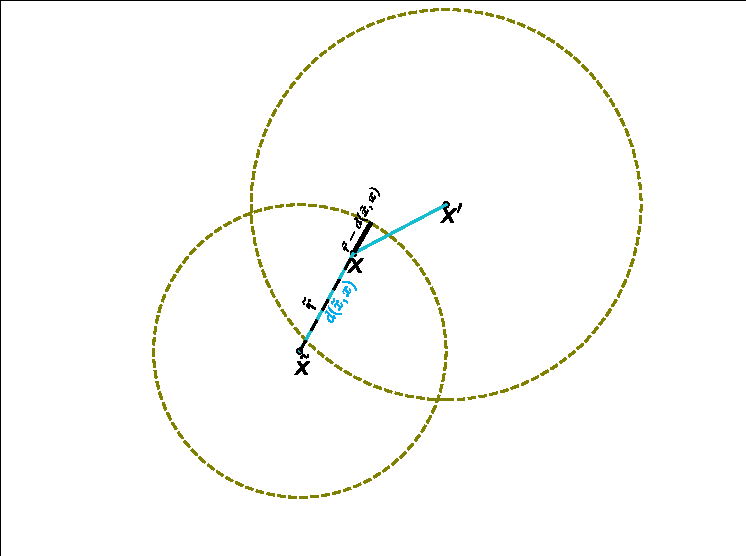
\includegraphics[trim={2.5cm 0.9cm 1.7cm 0.14cm}, clip, width=0.7\textwidth]{Figures/circles_modified.pdf}
			\caption{Any point in the intersection of two open balls lies in another open ball, which is contained in the intersection.}
			\label{fig:open_balls_intersection}
		\end{figure}
		If the intersection is empty, then the statement holds (vacuously). Let $x\in B_{\tilde{r}}(\tilde{x}) \cap B_{r'}(x')$, and thus $x\in B_{\tilde{r}}(\tilde{x})$ and $x\in B_{r'}(x')$. Define $r := \min\{ \tilde{r} - d(x, \tilde{x}), r' - d(x, x') \}$, and note that $x\in B_{r}(x)$. For all $y\in B_{r}(x)$, we have $d(y, \tilde{x}) \leq d(y, x) + d(x, \tilde{x}) < r + d(x, \tilde{x}) \leq \tilde{r}$, i.e. $y\in B_{\tilde{r}}(\tilde{x})$. Similarly, we can show $y\in B_{r'}(x')$, and thus $y\in B_{\tilde{r}}(\tilde{x})\cap B_{r'}(x')$, i.e. $B_{r}(x)\subset B_{\tilde{r}}(\tilde{x})\cap B_{r'}(x')$.
	\end{proof}
		
	 \begin{defn}[Closed ball]
		Let $(X, d)$ be a metric space, $\varphi\in X$ and $r > 0$. Then 
		\begin{align}
			B_{r}[\varphi] := \left\{ \psi\in X \vert d(\varphi, \psi) \leq r\right\} \subset X
		\end{align}
		is called a \textit{closed ball} in $X$ with middle point $\varphi$ and radius $r$.
	\end{defn}
	
	\begin{defn}[Open Set]
		\label{defn-open-set}
		Let $(X, d)$ be a metric space. Then a subset $U\subset X$ is called \textit{open} in $X$ if for every $\varphi \in U$ there is an open ball $B_{r}(\varphi)$ that is contained in $U$, i.e. $B_r(\varphi)\subset U$. 
	\end{defn}

	\begin{defn}[Closed Set]
		Let $(X, d)$ be a metric space. Then a subset $A\subset X$ is called \textit{closed} in $X$ if the complement $X\backslash A$ is open according to Definition \ref{defn-open-set}. 
	\end{defn}

	\begin{theorem}\label{open-balls-open}
		Open balls are open. 
	\end{theorem}
	
	\begin{proof}
		An illustration of the idea of the proof is shown in Figure. 
		\begin{figure}[h!]
			\centering
			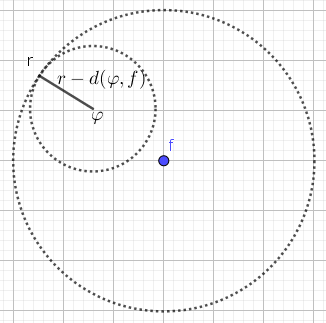
\includegraphics[width=0.35\textwidth]{Figures/open-balls-open.png}
		\end{figure}
		
		Let $f\in X$ and for $r > 0$ consider the open ball $U:= B_{r}(f) \subset X$. By definition, for every $\varphi \in U$ it holds that $d\left(\varphi, f\right) < r$. Now we show that 
		\begin{align}
			B_{r-d\left(\varphi, f\right)}(\varphi) \subset U.
		\end{align}
		For this consider $\psi\in B_{r-d\left(\varphi, f\right)}(\varphi)$, i.e. $d(\psi, \varphi) < r - d(\varphi, f)$. With the triangle inequality we obtain: 
		\begin{align}
			d(f, \psi) \leq d(f, \varphi) + d(\varphi, \psi) < d(f, \varphi) + r - d(\varphi, f) = r,  		
		\end{align}
		i.e. $d(f, \psi) < r$ and thus $\psi\in U = B_{r}(f)$.
	\end{proof}
	
	
	\begin{theorem}\label{thrm:closed_balls_open}
		Closed balls are closed.
	\end{theorem}
	
	\begin{proof}
		Let $f\in X$ and for $r > 0$ consider the closed ball $B_{r}[f]\subset X$. By definition, for every $\varphi \in X\backslash B_{r}[f]\subset X$, it holds that $d(\varphi, f) > r$. We will now show that 
		\begin{align}
			B_{d(\varphi, f) - r}(\varphi) \subset X \backslash B_{r}[f],
		\end{align}
		which would prove that $B_{r}[f]$ is closed. Let $\psi\in B_{d(\varphi, f) - r}(\varphi)$, i.e. $d(\psi, \varphi) < d(\varphi, f) -r$. With the triangle inequality, we obtain:
		\begin{align}
			d(f, \varphi) \leq d(f, \psi) + d(\psi, \varphi) \Leftrightarrow d(f, \psi) \geq d(f, \varphi) - d(\psi, \varphi) > d(f, \phi) - d(\varphi, f) + r = r, 
		\end{align}
		i.e. $d(f, \psi) > r$, and hence $\psi\notin B_r[f]$, implying that $\psi\in X\backslash B_{r}[f]$. 
	\end{proof}
	
	\begin{theorem}\label{thrm:open_sets_form_topology}
		Let $(X, d)$ be a metric space. The collection of open sets as in Definition \ref{defn-open-set} gives a topology.
	\end{theorem}
	\begin{proof}		
		According to Defn. \ref{defn:metric_space}, we need to prove that $X$ and $\emptyset$ are open, that the union of an arbitrary number of open sets is open, and that the intersection of a finite number of open sets is open. 
		
		Clearly, $X$ is open (since for any choice of $r > 0$ and $\varphi\in X$, $B_{r}(\varphi)\subset X$). $\emptyset$ is also open, since nothing needs to be shown.
		
		Now let $U_{1}$, $\dots$, $U_{n}\subset X$ be open, and consider the intersection
		\begin{align}
			U := \bigcap_{i=1}^{n}U_{i} \subset X.
		\end{align} 
		For any $\varphi\in U$, we know that $\varphi\in U_i$ for all $1\leq i \leq n$. Since the $U_{i}$ are open, there is a radius $r_{i} > 0$ such that $B_{r_i}(\varphi) \subset U_i$ for all $1\leq i \leq n$. Defining $r := \min_{1 \leq i \leq n}\{r_{i}\} > 0$, we have that $B_{r}(\varphi) \subset U_i$ for all $1\leq i\leq n$ and hence $B_{r}(\varphi)\subset U$.
		
		Finally, let $U_{i}$, $i\in I$, be open, where $I$ is in index set. Consider the union
		\begin{align}
			U := \bigcup_{i\in I}U_{i} \subset X.
		\end{align}
		For any $\varphi\in U$ there is an index $i\in I$ such that $\varphi\in U_i$. Since $U_i$ is open, there is an $r > 0$ such that $B_{r}(\varphi) \subset U_i \subset U$.
	\end{proof}

	\begin{defn}[Convergence of sequence \cite{fa2019}]\label{defn:convergence_sequence}
		Let $(X, d)$ be a metric space. A sequence $(\varphi_n)_{n\in\mathbb N}$ with elements $\varphi_n\in X$, $n\in\mathbb N$, is called \textit{convergent} if there is a $\varphi\in X$ s.t.
		\begin{align}
			\lim\limits_{n\to\infty}d(\varphi_n, \varphi) = 0,
		\end{align}
		i.e. for all $\epsilon > 0$ there exists an $N(\epsilon)\in\mathbb N$ s.t.
		\begin{align}
			d(\varphi_n, \varphi) < \epsilon \quad \forall n\geq N(\epsilon).
		\end{align}
		$\varphi$ is called the \textit{limit} of the sequence $(\varphi_n)_{n\in \mathbb N}$. For this, we write 
		\begin{align}
			\lim\limits_{n\to\infty}\varphi_n = \varphi \quad \text{or}\quad \varphi_n \overset{n \to\infty}{\longrightarrow} \varphi.
		\end{align}
		Non-convergent sequence are called \textit{divergent}.
	\end{defn}

	\begin{theorem}\label{thrm:sequences_unique_limits}
		Let $(X, d)$ be a metric space, and $\seq[\varphi_n]$ a convergent sequence in $X$ wrt $d$. Then the limit is unique.
	\end{theorem}

	\begin{proof}
		Assume the limit is not unique, i.e. $\seq[\varphi_n]$ converges to both $\varphi\in X$ and $\psi\in X$. with $\varphi\ne\psi$. Then for $\epsilon := d(\varphi, \psi) / 2$ there exists an $N'\in\mathbb N$ s.t. for all $n\geq N$, we have
		$$d(\varphi_n, \varphi) < \frac{d(\varphi, \psi)}{2} = \epsilon$$ 
		and an $\tilde{N}$ s.t. for all $n\geq \tilde{N}$, we have
		$$d(\varphi_n, \psi) < \frac{d(\varphi, \psi)}{2} = \epsilon.$$
		Define $N := \max\{N', \tilde{N}\}$, then for all $n\geq N$, we have
		$$d(\varphi, \psi) \leq d(\varphi, \varphi_n) + d(\varphi_n, \psi) < d(\varphi, \psi),$$
		which is a contradiction.
	\end{proof}

	\begin{theorem}\label{thrm:seq_convergence_subsequences}
		A sequence is convergent iff every subsequence converges to the same limit.
	\end{theorem}
	
	\begin{proof}[Proof \cite{213285}]
		\enquote{$\Longleftarrow$} Every sequence has a trivial subsequence, namely itself.
		
		\enquote{$\Longrightarrow$} Let $\left(\varphi_{n_k}\right)_{k\in\mathbb N}$ be a subsequence of $\seq[\varphi_n]$. Note that $n_k \geq k$ for all $k\in\mathbb N$, which we will prove by induction: Clearly, $n_1\geq 1$, and $n_k\geq k$ implies $n_{k + 1} > n_{k} \geq k$, i.e. $n_{k + 1}\geq k + 1$. 
		
		We denote the limit of $\seq[\varphi_n]$ by $\varphi$, and note that for all $\epsilon > 0$, there exists an $N\in\mathbb N$ s.t. for all $n \geq N$, we have $d(\varphi_n, \varphi) < \epsilon$. Thus, for all $k\geq N$ (and hence $n_k\geq N$), we have $d(\varphi_{n_k}, \varphi) < \epsilon$.
	\end{proof}

	\begin{defn}[Accumulation point]\label{defn:accumulation_point}
		Let $U\subset X$. Then $\varphi\in X$ is called an \textit{accumulation point} of $U$ if there is a sequence $\left(\varphi_{n}\right)_{n\in \mathbb N}$ in $U$ such that $\lim\limits_{n\to\infty}\varphi_{n} = \varphi$.
	\end{defn}

	\begin{theorem}\label{thm:closed_set_acc_point}
		A subset $U \subset X$ is closed if and only if it contains all its accumulation points according to Defn. \ref{defn:accumulation_point}.
	\end{theorem}

	\begin{proof}
		\enquote{$\Longleftarrow$}: Let $U$ contain all its accumulation points, and let $\varphi\in X\backslash U$. We will now show that there is an $n\in \mathbb N$ such that $B_{\frac{1}{n}}(\varphi) \subset X\backslash U$, proving that $X\backslash U$ is open. Assuming there is no such $n\in \mathbb N$, then $B_{\frac{1}{n}}(\varphi) \cap U = \emptyset$ for all $n\in \mathbb N$. This means that there is a sequence $(\varphi_{n})_{n\in\mathbb N}$ in $U$ such that $d(\varphi, \varphi_n) < \frac{1}{n}$ for all $n\in\mathbb N$. Hence, $\varphi$ is an accumulation point of $U$, and since $U$ contains all its accumulation points by assumption, it follows that $\varphi\in U$, contradicting the assumption that $\varphi\in X\backslash U$.
		
		\enquote{$\Longrightarrow$}: Let $U$ be closed, i.e. $X\backslash U$ is open. Further, let $\varphi\in X$ be an accumulation point of $U$, i.e. there is a sequence $(\varphi_n)_{n\in\mathbb N}$ in $U$ such that $\lim\limits_{n\to\infty}\varphi_n = \varphi$. Hence, by definition of convergence, for all $\epsilon > 0$ there exists an $n\in\mathbb N$ such that $\varphi_n\in B(\varphi, \epsilon) \cap U$, implying that $\varphi\in U$. Thus, $U$ contains all its accumulation points.
	\end{proof}
	
	\begin{defn}[Closure of set]\label{defn:closure_set}
		The set 
		\begin{align}
			\bar{U} := \{\varphi\in X\mid \varphi\ \text{is an accumulation point of}\ U\} \subset X
		\end{align}
		is called the closure of the set $U \subset X$.
	\end{defn}

	\begin{remark}\label{remark:closure_superset}
		Clearly, $U\subset \bar{U}$, since any $\varphi\in U$ is an accumulation point of $U$ (consider the constant sequence, where for any $n\in\mathbb N$, $\varphi_n := \varphi$).
	\end{remark}

	\begin{remark}
		According to Theorem \ref{thm:closed_set_acc_point}, a subset $U\subset X$ is closed if and only if it contains all its limit points, thus for a closed subset we have $\overline{U} \subset U$. With Remark \ref{remark:closure_superset}, we get $U$ is closed if and only if $U = \overline{U}$.
	\end{remark}
	
	\begin{theorem}\label{thrm:closure_closed}
		Let $U\subset X$. Then its closure, $\bar{U}$, is closed.
	\end{theorem}

	\begin{proof}
		According to Theorem \ref{thm:closed_set_acc_point}, we need to prove that $\bar{U}$ contains all its limit points. Let $\varphi\in X$ be an accumulation point of $\overline{U}$. Then for all $n\in \mathbb N$ there is a $\varphi_n\in\overline{U}$ such that $d(\varphi, \varphi_n) < 1/n$. By Def. \ref{defn:closure_set}, we also know that since $\varphi_n\in \bar{U}$, it is an accumulation point of $U$, i.e. for every $\varphi_n\in \overline{U}$ there is a $\psi_n\in U$ such that $d(\varphi_n, \psi_n) < 1/n$. Thus:
		\begin{align}
			d(\psi_n, \varphi) \leq d(\psi_n, \varphi_n) + d(\varphi_n, \varphi) < \frac{1}{n} + \frac{1}{n} \overset{n\to\infty}{\longrightarrow} 0,
		\end{align}
		i.e. $(\psi_n)_{n\in\mathbb N}$ is a sequence in $U$ that converges to $\varphi$, i.e. $\varphi$ is an accumulation point of $U$, hence $\varphi\in \bar{U}$.
	\end{proof}
	
	\begin{theorem}\label{thrm:property_metric_space}
		Let $(X, d)$ be a metric space. Then $\varphi\in \overline{U}$ for $U\subset X$ if and only if for every open set $O\subset X$ containing $\varphi$, $U\cap O\ne \emptyset$.
	\end{theorem}

	\begin{proof}
		\enquote{$\Longrightarrow$} Since $\varphi\in\overline{U}$, there exists a sequence $\left(\varphi_n\right)_{n\in\mathbb N}$ converging to $\varphi$ wrt $d$, i.e. for all $\epsilon > 0$ there exists an $N\in\mathbb N$ s.t. for all $n\geq N$, $d(\varphi_n, \varphi) < \epsilon$. Let $O\subset X$ be open, and let $\varphi\in O$. By definition, there exists an open ball $B_{r}(\varphi)\subset O$ with $r > 0$. Choose $\epsilon = r$ and $\psi = x_{N}\in U$, then $\psi\in B_{r}(\varphi) \subset O$.
		
		\enquote{$\Longleftarrow$} By assumption, for any non-empty open set $O\subset X$, $U\cap O\ne\emptyset$, where $U\subset X$. Let $\varphi\in X$. Since open balls are open, for any $\epsilon > 0$, $U\cap B_{\epsilon}(\varphi)\ne\emptyset$. Consider the sequence of open balls $\left( B_{1/n}(\varphi)\right)_{n\in\mathbb N}$, for which $U\cap B_{\frac{1}{n}}(\varphi) \ne \emptyset$ holds. Thus for each $n\in\mathbb N$, there exists a point $\varphi_{n}\in X$ s.t. $\varphi_n \in B_{\frac{1}{n}}(\varphi)$ and $\varphi_n\in U$. Hence, by definition, $\varphi\in X$ is an accumulation point of $U$.
	\end{proof}
	
	\begin{theorem}
		Let $U\subset X$. Then its closure, $\overline{U}$, is the \textit{smallest} closed set in $X$ containing $U$.
	\end{theorem}

	\begin{proof}
		From Remark \ref{remark:closure_superset}, we know that $U\subset \overline{U}$, and from Theorem \ref{thrm:closure_closed}, we know that $\overline{U}$ is closed. To prove that $\overline{U}$ is the smallest \textit{closed} set in $X$ containing $U$, let $V\subset X$ be another closed set that contains $U$, i.e. $U\subset V$. Every sequence in $U$ is also a sequence in $V$, i.e. every accumulation point of $U$ is in $V$, i.e. $\overline{U}\subset V$.
	\end{proof}

	\begin{defn}[Bounded set]\label{defn:bounded_set}
		A subset $U\subset X$ is called \textit{bounded} in $X$ if it is contained in a closed ball in $X$, i.e. there exists $r > 0$ and $\varphi \in X$ s.t. $U\subset B_{r}[\varphi]$.
	\end{defn}

	\begin{theorem}
		Convergent sequences in $X$ are fully contained in a bounded subset.
	\end{theorem}
	
	\begin{proof}
		Let $(\varphi_n)_{n\in\mathbb N}$ be a convergent sequence in $X$ with limit point $\varphi\in X$. Then there exists an $N\in\mathbb N$ s.t. $d(\varphi_n, \varphi) < \epsilon$ for all $n\geq N$ for a fixed $\epsilon > 0$. Defining
		\begin{align}
			r := \max \left\{ \epsilon, \max_{n \leq N}\{d(\varphi, \varphi_n)\} \right\},
		\end{align}
		we have $d(\varphi, \varphi_n) \leq r$ for all $n\in\mathbb N$. Hence, for any $n\in\mathbb N$, 
		$\varphi_n\in B_{r}[\varphi]$.¸
	\end{proof}
	
	\begin{defn}[Isometry]
		Let $(X, d)$ and $(X', d')$ be metric spaces. Then $f: X \rightarrow Y$ is called a distance-preserving map (or \textit{isometry}) if
		\begin{align}
			d'(f(\varphi), f(\psi)) = d(\varphi, \psi) \quad\forall \varphi, \psi\in X
		\end{align}
		$(X, d)$ and $(X', d')$ are called \textit{isometric} if there is a surjective isometry $f:X\rightarrow X'$.
	\end{defn}

	\begin{theorem}\label{thrm:isometries_injective}
		Let $(X, d)$ and $(X', d')$ be metric spaces and $f: X\rightarrow X'$  be an isometry. Then it is injective.
	\end{theorem}

	\begin{proof}
		If $f(\varphi) = f(\psi)$ for any $\varphi$, $\psi\in X$, then 
		\begin{align}
			d'(f(\varphi), f(\psi)) = d'(f(\varphi), f(\varphi)) = d(\varphi, \psi) = 0, 
		\end{align}
		i.e. $\varphi = \psi$.
	\end{proof}

	\begin{remark}
		Two isometric spaces $(X, d)$ and $(X', d')$ do not differ in their properties wrt their metrics, but instead in the properties of their individual elements. Any metric property holding in one metric space also holds in the other. Hence, in this sense, we say that $(X, d)$ and $(X', d')$ are \textit{identical}.
	\end{remark}
	
	\begin{remark}
		Surjective isometries are hence bijective.
	\end{remark}
	
	\subsection{Complete metric spaces}
	
	\begin{defn}
		A sequence $(\varphi_n)_{n\in\mathbb N}$ in a metric space $(X, d)$ is a \textit{Cauchy sequence} if 
		\begin{align}
			\lim\limits_{n, m\to\infty} d(\varphi_n, \varphi_m) = 0,
		\end{align}
		i.e. for all $\epsilon > 0$ there exists an $N(\epsilon)\in \mathbb N$ s.t. 
		\begin{align}
			d(\varphi_n, \varphi_m) < \epsilon \quad\forall n, m\geq N.
		\end{align}
	\end{defn}

	\begin{theorem}\label{thrm:convergent_sequence_cauchy_sequence}
		Every convergent sequence in $X$ is a cauchy sequence in $X$.
	\end{theorem}

	\begin{proof}
		Let $(\varphi_n)_{n\in\mathbb N}$ be a convergent sequence in $X$ with limit point $\varphi\in X$. Hence, for all $\epsilon > 0$, there is an $N(\epsilon)\in\mathbb N$ with $d(\varphi_n, \varphi) < \epsilon$ for all $n\geq N(\epsilon)$. Hence
		\begin{align}
			d(\varphi_n, \varphi_m) \leq d(\varphi_n, \varphi) + d(\varphi, \varphi_m) < 2\epsilon \quad\forall n,m\geq N.
		\end{align}
	\end{proof}

	\begin{theorem}\label{thrm:cauchy_convergent_subsequence}
		A Cauchy sequence in a metric space $(X, d)$ is convergent iff it contains a convergent subsequence.
	\end{theorem}

	\begin{proof}[Proof \cite{354965}]
		\enquote{$\Longrightarrow$} Every sequence has a trivial subsequence, namely itself.
		
		\enquote{$\Longleftarrow$} Let $\left(\varphi_{n_k}\right)_{k\in\mathbb N}$ be a subsequence of the Cauchy sequence $\seq[\varphi_n]$, and assume that $\lim\limits_{k\to\infty}\varphi_{n_k} = \varphi$ wrt $d$, where $\varphi\in X$, i.e. for all $\epsilon > 0$ there exists an $N'\in\mathbb N$ s.t. for all $k\geq N'$, $d(\varphi_{n_k}, \varphi) < \epsilon$ (note that $n_k \geq k$). Since $\seq[\varphi_n]$ is Cauchy, there exists an $\tilde{N}$ s.t. for all $m, n\geq \tilde{N}$, we have $d(\varphi_n, \varphi_m) < \epsilon$. Define $N := \max\left\{N', \tilde{N}\right\}$, then for all $k, n\geq N$,
		\begin{align*}
			d(\varphi_n, \varphi) \leq d(\varphi_n, \varphi_{n_k}) + d(\varphi_{n_k}, \varphi) < 2\epsilon,
		\end{align*}
		and thus $\seq[\varphi_n]$ converges to $\varphi$.
	\end{proof}

	\begin{remark}\label{remark:cauchy_not_convergent_necess}
		The converse of Theorem \ref{thrm:convergent_sequence_cauchy_sequence} is in general not true: Take $X=\mathbb Q$ and let $d(x, y) := \abs{x - y}$, for any $x$, $y\in\mathbb Q$. Then we have a metric space $(\mathbb Q, d)$, but the sequence $(a_n)_{n\in\mathbb N}$ with
		\begin{align}\label{eq:seq_euler}
			a_n := \left(1 + \frac{1}{n}\right)^n,
		\end{align}
		which is a Cauchy sequence and where all elements are in $\mathbb Q$, does not converge in $\mathbb Q$ (the limit point is Euler's number $e$). To prove this, we will make use of the following two Theorems.
	\end{remark}
	
	\begin{theorem}\label{thrm:mono_inc_seq_Cauchy}
		Any sequence $(a_n)_{n\in\mathbb N}$ with $a_n\in \mathbb R$ for any $n\in \mathbb N$ that is monotonically increasing and upper bounded for any $n\in\mathbb N$ is a Cauchy sequence in ($\mathbb R$, $d$) with $d(x, y):= \abs{x - y}$ for any $x$, $y\in \mathbb R$.		
	\end{theorem}

	\begin{proof}(\cite{2169936})
		The completeness axiom states that any non-empty subset of $\mathbb R$ that has an upper bound has a least upper bound in $\mathbb R$. Let $M$ be the least upper bound for the sequence $(a_n)_{n\in\mathbb N}$, i.e. $a_n \leq M$ for all $n\in\mathbb N$. Since $M$ is the least upper bound, for all $\epsilon > 0$ there is an $N\in\mathbb N$ s.t. $M - \epsilon < a_N \leq M$.
		
		By assumption, the sequence is monotonically increasing, i.e. $a_m \geq a_n$ for any $m > n$. Without loss of generality, let $m > n$, then we have
		\begin{align}\label{eq:mono_inc_seq_Cauchy}
			M - \epsilon < a_N \leq a_n \leq a_m \leq M, \quad \forall (m, n\geq N) \wedge (m > n)
		\end{align}
		from which $a_m - a_n < \epsilon$ follows. Similarly, we can show that $a_n - a_m < \epsilon$ for $n > m$. Hence, $d(a_m, a_n) < \epsilon$ for any $m$, $n\geq N$.
	\end{proof}
	
	\begin{theorem}\label{thrm:AM-GM}
		Let $x_1$, \dots, $x_n\in\mathbb R_{\geq 0}$, $n\geq 1$, then the arithmetic mean is bigger than or equal to the geometric mean, i.e.
		\begin{align}\label{eq:AM-GM}
			\frac{\sum_{i=1}^{n} x_i}{n} \geq \left(\prod_{i=1}^{n}x_i\right)^{1/n}
		\end{align}
	\end{theorem}
	
	\begin{proof}(\cite{Wiki:AM-GM})
		Via induction. Let $n=1$, then $x_1 \geq x_1$, which is true. 
		
		Assuming that Eq. \eqref{eq:AM-GM} holds for any $n\in\mathbb N$, we will make the transition $n\mapsto n + 1$ and denote the arithmetic mean of $x_1$, \dots, $x_{n + 1}$ by $\alpha$:
		\begin{align}\label{eq:AM-GM-proof-1}
			(n + 1) \alpha = \sum_{i=1}^{n + 1} x_i \Leftrightarrow n\alpha = \sum_{i=1}^{n + 1}x_i - \alpha
		\end{align}
		If $x_i = \alpha$ for all $1\leq i\leq n + 1$, then we are done, since Eq. \eqref{eq:AM-GM} would be an equality. If all the $x_i$ are not equal to $\alpha$, then WLOG, let there be exactly two $x_i$ that are not equal to $\alpha$. Place these two elements at the end, and noting that one needs to be bigger than $\alpha$ and the other smaller than $\alpha$, WLOG we have 
		\begin{align}\label{eq:AM-GM-proof-2}
			\left(x_n - \alpha > 0\right) \wedge \left( \alpha - x_{n+1} > 0 \right) \Rightarrow (x_n - \alpha)(\alpha - x_{n+1}) > 0.
		\end{align}
		Now define
		\begin{align}
			y := x_{n} + x_{n + 1} - \alpha \geq x_{n} - \alpha \overset{\tiny\eqref{eq:AM-GM-proof-2}}{>} 0.
		\end{align}
		and substitute it into Eq. \eqref{eq:AM-GM-proof-1}:
		\begin{align}
			n\alpha = \sum_{i=1}^{n + 1}x_i - \alpha = \sum_{i=1}^{n-1}x_i + x_n + x_{n+1} - \alpha = \sum_{i=1}^{n-1}x_i + y
		\end{align}
		Thus, $\alpha$ is also the arithmetic mean of the $n$ numbers $x_1$, \dots, $x_{n-1}$, $y$. Making use of the induction hypothesis, we get
		\begin{align}\label{eq:AM-GM-proof-3}
			\alpha^{n+1} = \alpha\alpha^n \geq \alpha y\prod_{i=1}^{n-1} x_i.
		\end{align}
		From Eq.\eqref{eq:AM-GM-proof-2} we know that 
		\begin{align}\label{eq:AM-GM-proof-4}
			y\alpha - x_{n}x_{n+1} = (x_{n} + x_{n + 1} - \alpha)\alpha - x_{n}x_{n+1} = (x_n - \alpha)(\alpha - x_{n+1}) > 0 \Leftrightarrow y\alpha > x_{n}x_{n+1}
		\end{align}
		Substituting Eq. \eqref{eq:AM-GM-proof-4} into \eqref{eq:AM-GM-proof-3}, we get
		\begin{align}
			\alpha^{n+1} \geq \alpha y\prod_{i=1}^{n-1} x_i > x_nx_{n+1}\prod_{i=1}^{n-1} x_i = \prod_{i=1}^{n + 1} x_i \Leftrightarrow \alpha \geq \left(\prod_{i=1}^{n+1}x_i\right)^{\frac{1}{n+1}},
		\end{align}
		which proves the induction hypothesis.
	\end{proof}
	
	\begin{proof}(of Remark \ref{remark:cauchy_not_convergent_necess}) 
		Looking at the proof of Theorem \ref{thrm:mono_inc_seq_Cauchy}, we will see that that the statement of Theorem \ref{thrm:mono_inc_seq_Cauchy} also holds for sequences in $\mathbb Q$ that are upper bounded and monotonically increasing, since any non-empty subset of $\mathbb Q\subset \mathbb R$ that is upper bounded has a least upper bound in $\mathbb R$ (though not necessarily in $\mathbb Q$). 
		
		Hence, to show that the sequence $(a_n)_{n\in\mathbb N}$ with $a_n = \left(1 + n^{-1}\right)^n$ is a Cauchy sequence in $\mathbb Q$, we only need to show that it is monotonically increasing and derive an upper bound.
			
		For the monotonicity, we will make use of Theorem \ref{thrm:AM-GM} (\cite{64864}). For this, define the $x_i$ as follows: 
		\begin{align}
			x_i := \begin{cases}
				1, & i = 1
				\\ 1 + \frac{1}{n}, & 2 \leq i \leq n + 1
			\end{cases}
		\end{align}
		Then we have
		\begin{align}
			\frac{\sum_{i=1}^{n + 1}x_i}{n + 1} &\geq \left(\prod_{i = 1}^{n + 1}x_i\right)^{\frac{1}{n+1}} 
			\Leftrightarrow \left(\frac{\sum_{i=1}^{n + 1}x_i}{n + 1}\right)^{n+1} \geq \prod_{i = 1}^{n + 1}x_i
			\\ \Rightarrow \left(\frac{1 + n\left(1 + \frac{1}{n}\right)}{n+1}\right)^{n + 1} &= \left(1 + \frac{1}{n + 1}\right)^{n + 1} \geq \left(1 + \frac{1}{n}\right)^n \quad\forall n\in\mathbb N,
		\end{align}
		i.e. $a_{n+1} > a_n$.
		
		To prove that the sequence $(a_n)_{n\in\mathbb N}$ is upper bounded (\cite{5065619}), note that
		\begin{align}
			a_n &= \left(1 + \frac{1}{n}\right)^n = \sum_{k=0}^{n}\begin{pmatrix}
				n \\ k
			\end{pmatrix}\frac{1}{n^k} = \sum_{k = 0}^{n}\frac{n!}{k!(n-k)!}\frac{1}{n^k} = 1 + \sum_{k = 1}^{n}\frac{n!}{k!(n-k)!}\frac{1}{n^k}
			\\ &= 1 + \sum_{k = 1}^{n}\frac{n(n-1)\dots (n-k+1)}{k!}\frac{1}{n^k} \leq 1 + \sum_{k=1}^{n}\frac{1}{k!} \leq 1 + \sum_{k=1}^{n}\frac{1}{2^{k-1}}
			\\ &\leq 1 + \sum_{k=0}^{\infty}\frac{1}{2^k} = 3.
		\end{align}
	\end{proof}

	\begin{exmp}
		We can instruct infinitely many counter-examples to Theorem \ref{thrm:convergent_sequence_cauchy_sequence} in $\mathbb Q$. Let 
		\begin{align}
			\left(a_n\right)_{n\in\mathbb N} := \floor{10^{n} \cdot a}\cdot 10^{-n}, 
		\end{align}
		where $a\in \mathbb R\backslash \mathbb Q$. $(a_n)_{n\in\mathbb N}$ is a Cauchy sequence in $\mathbb Q$, which gives $a$ to its $n^{\text{th}}$ decimal point, converging to $a$. To see that it is a Cauchy sequence in $\mathbb Q$, note that all sequence elements are rational, that the sequence is bounded by $a$ and that it is monotonically increasing. Thus, by the proof of Theorem \ref{thrm:mono_inc_seq_Cauchy}, which also holds for $\mathbb Q$, $\left(a_n\right)_{n\in\mathbb N}$ is Cauchy in $\mathbb Q$.
	\end{exmp}

	\begin{theorem}\label{thrm:mono_inc_seq_converges}
		Any sequence $(a_n)_{n\in\mathbb N}$ with $a_n\in \mathbb R$ for any $n\in \mathbb N$ that is monotonically increasing and upper bounded for any $n\in\mathbb N$ converges in ($\mathbb R$, $d$) with $d(x, y):= \abs{x - y}$ for any $x$, $y\in \mathbb R$.
	\end{theorem}

	\begin{proof}
		The proof is identical to that of Theorem \ref{thrm:mono_inc_seq_Cauchy}. With the same notation as there, we have, cf. Eq. \eqref{eq:mono_inc_seq_Cauchy}:
		\begin{align}
			M - \epsilon &< a_n \leq M, \quad \forall n\geq N
			\\ \Rightarrow \abs{a_n - M} &< \epsilon,
		\end{align}
		i.e. the limit point of $(a_n)_{n\in\mathbb N}$ is $M$ (the least upper bound).
	\end{proof}

	\begin{remark}
		Note that Theorem \ref{thrm:mono_inc_seq_converges} does not hold in $\mathbb Q$, since the completeness axiom only guarantess the existence of a least upper bound in $\mathbb R$.
	\end{remark}

	\begin{theorem}\label{thrm:cauchy_sequences_bounded}
		Let $(X, d)$ be a metric space. Then if $\seq[\varphi_n]$ is a Cauchy sequence, it is bounded.
	\end{theorem}

	\begin{proof}
		Fix $\epsilon > 0$ and $\psi\in X$. Since $\seq[\varphi_n]$ is a Cauchy sequence, there exists an $N\in\mathbb N$ s.t. $d(\varphi_m, \varphi_n) <\epsilon$ for all $m, n\geq N$. Define
		\begin{align}
			M := \max_{1\leq i\leq N}\left\{ d(\psi, \varphi_n) \right\}, 
		\end{align}
		and note that the maximum exists since we take it over a set with finitely many elements. For $n\leq N$, we obviously have $d(\psi, \varphi_n)\geq M$. For $n > N$, we have
		\begin{align*}
			d(\psi, \varphi_n) \leq d(\psi, \varphi_N) + d(\varphi_N, \varphi_n) < M + \epsilon.
		\end{align*}
		Thus, $\seq[\varphi_n]$ is contained in $B_{M + \epsilon + 1}[\psi]$.
	\end{proof}

	\begin{defn}
		Let $(X, d)$ be a metric space. Then $(X, d)$ is called \textit{complete} if every Cauchy sequence in $X$ converges to a $\varphi\in X$ wrt $d$.
	\end{defn}
	
	\begin{theorem}
		Let $(X, d)$ be a metric space and consider the set $Y$. If $f: X\to Y$ is a bijection, then we can endow $Y$ with the following metric $d'$:
		\begin{align}\label{eq:metrics_completion}
			d'(y_1, y_2) := d\left(f^{-1}(y_1), f^{-1}(y_2)\right). \quad \forall y_1, y_2\in Y
		\end{align}
		$(X, d)$ is complete iff $(Y, d')$ is complete \cite{3789234}.
	\end{theorem}
	
	\begin{proof}
		Let $(X, d)$ be complete, i.e. every Cauchy sequence in $X$ converges in $X$. Now let $(x_n)_{n\in\mathbb N}$ be a Cauchy sequence in $X$ with limit point $\varphi\in X$. Consider the sequence $(y_n)_{n\in\mathbb N} := \left(f(x_n)\right)_{n\in\mathbb N}$ in $Y$. Since $X$ is Cauchy, we have $ d(x_m, x_n) = d'(y_m, y_n) < \epsilon$ for all $\epsilon > 0$ and $m$, $n\geq N$. Thus, we have that $(y_{n})_{n\in\mathbb N}$ is also a Cauchy sequence in $Y$. The limit point of $\left(y_n\right)_{n\in\mathbb N}$ is $f(\varphi)$, since $d'(y_n, f(\varphi)) = d(x_n, \varphi) < \epsilon'$ for all $\epsilon' > 0$ and $n\geq N'$.
	\end{proof}

	\begin{remark}
		To construct incomplete metric spaces, we can thus take an incomplete metric space $(X, d)$, construct a surjection $f:X\to Y$ to another set $Y$ and endow $Y$ with the metric $d'$ from Eq. \eqref{eq:metrics_completion}, then $(Y, d')$ is also incomplete.
	\end{remark}
	
	\begin{exmp}\label{exmp:r_with_arctan_metric}
		Let $X = \left(-\frac{\pi}{2}, \frac{\pi}{2}\right)$, and consider the metric $d(x_1, x_2) := \abs{x_1 - x_2}$. Define $Y = \mathbb R$, and consider the map $f: X\to Y$, $x\mapsto \tan(x)$, which is surjective. On $Y$, consider the metric $d'(y_1, y_2) := d\left( \arctan(y_1), \arctan(y_2)\right) = \abs{\arctan y_1 - \arctan y_2}$, cf. Eq. \eqref{eq:metrics_completion}. Since $(X, d)$ is incomplete, $(Y, d')$ is incomplete as well. To see that $(X, d)$ is incomplete, note that $\left(\frac{\pi}{2} - \frac{1}{n}\right)_{n\in\mathbb N}$ or $\left( -\frac{\pi}{2} + \frac{1}{n} \right)_{n\in\mathbb N}$ are Cauchy in $X$, yet do not converge in $X$.
	\end{exmp}
	
	\begin{exmp}[Complete metric spaces]
		Any set $X$ equipped with the discrete metric from Def. \ref{remark:discrete-metric} is complete.
	\end{exmp}
	
	\begin{exmp}
		The metric space $(\mathbb R, d)$ with $d(x, y) := \abs{x - y}$ is \mbox{complete}. Also, $(\mathbb R^{d}, \norm{x}{p})$, cf. Example \ref{exmp:lp-norm-vectors}, for $1\leq p\leq \infty$ is complete.
	\end{exmp}

	\begin{exmp}\label{exmp:space-continuous-functions-complete}
		Let $\mathcal C[a, b]$ be the space of all continuous functions $\chi: [a, b]\to\mathbb{R}$ with the metric 
		\begin{align}
			d_{\infty}(\varphi, \psi) = \norm{\varphi - \psi}{\infty} :=  \sup_{x\in [a, b]}\left\{ \abs{\varphi(x) - \psi(y)} \right\}\quad \forall \varphi, \psi\in\mathcal C[a, b].
		\end{align}
		The metric space $(\mathcal C[a, b], d_{\infty})$ is complete.
	\end{exmp}

	\begin{proof}
		Let $(\varphi_n)_{n\in\mathbb N}$ be a Cauchy sequence in $\mathcal C[a, b]$, then for any $x\in [a, b]$:
		\begin{align}
			\abs{\varphi_n(x) - \varphi_m(x)} \leq \sup_{x\in [a, b]}\left\{ \abs{\varphi_{n}(x) - \varphi_{m}(y)} \right\} < \epsilon. \quad\forall m, n\geq N
		\end{align} 
		Hence, $(\varphi_n)_{n\in\mathbb N}(x)$ is a Cauchy sequence in $\mathbb R$ for any $x\in[a, b]$ wrt the metric $d(x, y) := \abs{x - y}$. Since $\left(\mathbb R, d\right)$ is complete, we know that $\varphi(x) := \lim\limits_{n\to\infty}\varphi_n(x)$ exists. 
		
		Finally, let us show that $\varphi\in\mathcal C[a, b]$. Since $\left(\varphi_n(x)\right)_{n\in\mathbb N}$ converges in $(\mathbb R, d)$, we can choose an $N\in\mathbb N$ s.t. $\abs{\varphi_n(x) - \varphi(x)} < \epsilon/3$ for all $n\geq N$ and all $x\in[a, b]$. And since $\left(\varphi_n\right)_{n\in\mathbb N}$ is a Cauchy sequence in $(\mathcal C[a, b], d_{\infty})$ (by assumption), i.e. the $\varphi_n$ are continuous, there exists a $\delta > 0$ s.t. $\abs{\varphi_N(x) - \varphi_{N}(y)} < \epsilon/3$ with $\abs{x - y} < \delta$. If $\abs{x-y} < \delta$, we get by applying the triangle inequality
		\begin{align}
			\abs{\varphi(x) - \varphi(y)} \leq \abs{\varphi(x) - \varphi_N(x)} + \abs{\varphi_N(x) - \varphi_N(y)} + \abs{\varphi_N(y) - \varphi(y)} < \epsilon,
		\end{align}
		which shows the continuity of $\varphi$, cf. Def. \ref{defn:continuity}.
		
		Thus, we have shown that $\varphi\in\mathcal C[a, b]$.
	\end{proof}
	
	\begin{remark}
		Let $(X, d)$ be a metric space. Then if $\seq[\varphi_n]$ and $\seq[\psi_n]$ are Cauchy sequences in $(X, d)$, their sum $\seq[\varphi_n + \psi_n]$ is \textit{not} necessarily a Cauchy sequence in $X$ wrt $d$. (Note that we are assuming here that $X$ is equipped with a binary operation $+$.)
	\end{remark}

	\begin{exmp}\label{exmp:counter_exmp_sum_Cauchy_not_Cauchy}
		Consider the metric space $(\mathbb R, d)$ with $d(x, y) := \abs{\arctan x - \arctan y}$ for any $x$, $y\in\mathbb R$, cf. Example \ref{exmp:r_with_arctan_metric}. Define the sequences $\seq[a_n]$ as $a_n := n$ and $\seq[b_n]$ as $b_n := (-1)^n - n$. Note that both sequences are Cauchy, but $\seq[a_n + b_n] = \seq[(-1)^n]$ is not.
	\end{exmp}

	\begin{remark}
		Let $(X, d)$ be a metric space. Then if $\seq[\varphi_n]$ and $\seq[\psi_n]$ are Cauchy sequences in $(X, d)$, their product $\seq[\varphi_n \cdot \psi_n]$ is \textit{not} necessarily a Cauchy sequence in $X$ wrt $d$. (Note that we are assuming here that $X$ is equipped with a binary operation $\cdot$.)
	\end{remark}

	\begin{exmp}\label{exmp:counter_exmp_prod_Cauchy_not_Cauchy}
		Consider the metric space $(\mathbb R, d)$ with $d(x, y) := \abs{\arctan x - \arctan y}$ for any $x$, $y\in\mathbb R$, cf. Example \ref{exmp:r_with_arctan_metric}. Define the sequences $\seq[a_n]$ as $a_n := n$ and $\seq[b_n]$ as $b_n := \frac{(-1)^n}{n}$. Note that both sequences are Cauchy, but $\seq[a_n \cdot b_n] = \seq[(-1)^n]$ is not.
	\end{exmp}
	
	\begin{remark}
		In the special case of $X = \mathbb Q$ or $X = \mathbb R$ with $d(x, y) := \abs{x - y}$ for any $x$, $y\in X$, then the sum and product of two Cauchy sequences is indeed Cauchy again, cf. Theorem \ref{thrm:sum_Cauchy_sequences_Cauchy} and \ref{thrm:prod_Cauchy_sequences_Cauchy}.
	\end{remark}
	
	\begin{proof}[Proof of Example \ref{exmp:counter_exmp_sum_Cauchy_not_Cauchy}]
		First, we will show that $\seq[a_n] = \seq[n]$ is Cauchy. For any $\epsilon > 0$, choose $N = N(\epsilon)$ s.t. $N > 1/\epsilon$, and note that for any $m$, $n\geq N$, we have
		\begin{align}\label{eq:arctan_cauchy_exmp}
			d(a_m, a_n) = \abs{\arctan m - \arctan n} = \abs{\arctan\left(\frac{m - n}{1 + mn}\right)} \overset{(\star)}{\leq} \abs{\frac{m - n}{1 + mn}} \leq \frac{\abs{m - n}}{mn},
		\end{align}
		where the inequality in $(\star)$ can be obtained by using the integral definition of $\arctan x$. WLOG assume $n\leq m$, then Equation \eqref{eq:arctan_cauchy_exmp} can be further simplified to
		\begin{align*}
			d(a_m, a_n) \overset{\tiny\eqref{eq:arctan_cauchy_exmp}}{\leq} \frac{\abs{m - n}}{mn} \leq \frac{m}{mn} \overset{n\geq N}{\leq}\frac{m}{mN} = \frac{1}{N} \overset{N > \epsilon^{-1}}{<} \epsilon. 
		\end{align*}
		To show that $\seq[b_n] = \seq[(-1)^n - n]$ is Cauchy, choose $N = N(\epsilon)$ s.t. $N > \frac{1}{\epsilon} + 2$, and note that for $m$, $n\geq N$, we have
		\begin{align}
			d(b_m, b_n) &= \abs{\arctan\left((-1)^m - m\right)} - \abs{\arctan\left((-1)^n - n\right)} \\[2pt] &= \abs{\arctan\left( \frac{(-1)^m - m - (-1)^n+n}{1 + \left((-1)^m - m\right) \cdot \left((-1)^n -n\right) } \right)} 
			\\[2pt] &\leq \abs{\frac{(-1)^m - m - (-1)^n+n}{1 + \left((-1)^m - m\right) \cdot \left((-1)^n -n\right) }} 
			\\[2pt] &= \abs{\frac{1}{1 + \left((-1)^m - m\right) \cdot \left((-1)^n -n\right)}}\cdot \abs{(-1)^m - m - (-1)^n+n}
			\\[2pt] &\leq  \abs{\frac{1}{1 + \left((-1)^m - m\right) \cdot \left((-1)^n -n\right)}}\abs{n - m} 
			\\[2pt] &= \abs{\frac{m - n}{1 + (-1)^{m + n} - m \cdot (-1)^n -n\cdot (-1)^m + mn}}
			\\[2pt] &\leq \abs{\frac{m - n}{- m \cdot (-1)^n -n\cdot (-1)^m + mn}} \label{eq:arctan_cauchy_exmp_2}
		\end{align}
		We will distinguish four cases:
		\begin{enumerate}
			\item If $m$ and $n$ are both uneven, then Eq. \eqref{eq:arctan_cauchy_exmp_2} becomes 
			\begin{align*}
				d(b_m, b_n) &\overset{\tiny\eqref{eq:arctan_cauchy_exmp_2}}{\leq} \abs{\frac{m - n}{- m \cdot (-1)^n -n\cdot (-1)^m + mn}}
				\\[2pt] &= \abs{\frac{m - n}{m + n + mn}} \leq \abs{\frac{m - n}{nm}},
			\end{align*}
			which reduces to showing that $\seq[a_n]$ is Cauchy, cf. Eq. \eqref{eq:arctan_cauchy_exmp}.
			
			\item If $m$ and $n$ are both even and WLOG we assume $n\leq m$, then Eq. \eqref{eq:arctan_cauchy_exmp_2} becomes
			\begin{align*}
				d(b_m, b_n) &\overset{\tiny\eqref{eq:arctan_cauchy_exmp_2}}{\leq} \abs{\frac{m - n}{- m \cdot (-1)^n -n\cdot (-1)^m + mn}}
				\\[2pt] &= \abs{\frac{m - n}{-m-n+mn}} \overset{n\leq m}{\leq} \frac{m}{\abs{-m -n + mn}} = \frac{1}{\abs{-1 -\frac{n}{m} + n}}
				\\[2pt] &\overset{(\star)}{=} \frac{1}{-1-\frac{n}{m} + n} \overset{(\diamond)}{\leq}\frac{1}{n - 2} \overset{n\geq N}{\leq} \frac{1}{N - 2} \overset{N > \epsilon^{-1} + 2}{<} \epsilon,
			\end{align*} 
			where the equality in $(\star)$ and the inequality in $(\star)$ follow from $n\geq N > 2$ and $n\leq m$, since 
			\begin{align*}
				n \leq m \Rightarrow \frac{n}{m} \leq 1\Rightarrow -1- \frac{n}{m} + n\geq n - 2 > 0.
			\end{align*}
		
			\item If $m$ is uneven and $n$ is even and WLOG we asumme $n\leq m$, then we have
			\begin{align*}
				d(b_m, b_n) &\overset{\tiny\eqref{eq:arctan_cauchy_exmp_2}}{\leq} \abs{\frac{m - n}{- m \cdot (-1)^n -n\cdot (-1)^m + mn}} = \abs{\frac{m - n}{-m + n + mn}}
				\\[2pt] &\overset{n\leq m}{\leq} \frac{m}{\abs{n - m + mn}} = \frac{1}{\abs{\frac{n}{m} - 1 + n}} = \frac{1}{\frac{n}{m} - 1 + n} \leq \frac{1}{n - 1}
				\\[2pt] &\overset{n \geq N}{\leq} \frac{1}{N - 1} \overset{N > \epsilon^{-1} + 2}{<} \epsilon.
			\end{align*}
			
			\item If $m$ is even and $n$ is uneven, proceed similarly to 3.
		\end{enumerate}
		Finally, note that it is obvious that $\seq[a_n + b_n] = \seq[(-1)^n]$ is not Cauchy.
	\end{proof}
	
	\begin{proof}[Proof of Example \ref{exmp:counter_exmp_prod_Cauchy_not_Cauchy}]
		We have already shown in the proof of Example \ref{exmp:counter_exmp_sum_Cauchy_not_Cauchy} that $\seq[a_n] = \seq[n]$ is Cauchy wrt $d(x, y) := \abs{\arctan x - \arctan y}$ for any $x$, $y\in\mathbb R$. To show that $\seq[b_n] = \seq[\frac{(-1)^n}{n}]$ is Cauchy wrt $d$, choose $N = N(\epsilon) > \frac{2}{\epsilon}$, then we have for any $m$, $n\geq N$:
		\begin{align*}
			d(b_m, b_n) &= \abs{\arctan\left(\frac{(-1)^m}{m}\right) - \arctan \left(\frac{(-1)^n}{n}\right)} 
			\\[2pt] &\leq \abs{\arctan\left(\frac{(-1)^m}{m}\right)} + \abs{\arctan\left(\frac{(-1)^n}{n}\right)} 
			\\[2pt] &\leq \abs{\frac{(-1)^m}{m}} + \abs{\frac{(-1)^n}{n}} = \frac{1}{m} + \frac{1}{n} \\[2pt] &\overset{\text{\tiny WLOG}\ n \leq m}{\leq} \frac{2}{n} \overset{n \geq N}{\leq} \frac{2}{N} \overset{N > 2\epsilon^{-1}}{<} \epsilon.
		\end{align*}
	\end{proof} 
	
	\begin{theorem}\label{thrm:complete_subsets_properties}
		Let $(X, d)$ be a metric space. Then the following statements are true.
		\begin{enumerate}[label=(\alph*)]
			\item Complete subsets of $(X, d)$ are closed. \vspace{-0.3cm}
			\item If $(X, d)$ is complete, then every closed subset of $(X, d)$ is complete.
		\end{enumerate}
	\end{theorem}

	\begin{proof}
		(a): Let $U\subset X$ be closed wrt $d$, and let $\varphi\in X$ be a limit point of $\overline{U}$, i.e. there exists a sequence $\left(\varphi_{n}\right)_{n\in\mathbb N}$ in $U$ s.t. $\lim\limits_{n\to\infty}\varphi_n = \varphi$. Hence, $\left(\varphi_{n}\right)_{n\in\mathbb N}$ converges in $X$, and is thus a Cauchy sequence in $X$. Since $U$ is closed, the limit of the sequence lies in $U$, i.e. $U$ is closed.
		
		(b): Let $(X, d)$ be complete, $U\subset X$ closed and $(\varphi_n)_{n\in\mathbb N}$ a Cauchy sequence in $U$, which converges to a $\varphi\in X$, since $X$ is closed. Since $\varphi$ is the limit of $(\varphi_n)_{n\in\mathbb N}$ and $U$ is closed, it follows that $\varphi\in U$.
	\end{proof}

	\begin{defn}
		Let $(X, d)$ be a metric space. Then $U\subset X$ is called \textit{dense} in $X$ if $\overline{U} = X$, i.e. to every $\varphi\in X$ there exists a sequence $\left(\varphi_n\right)_{n\in\mathbb N}$ in $U$ that converges to $\varphi$ wrt $d$. Alternatively, we can say that to every $\varphi\in X$ and $\epsilon > 0$ there is a $\psi\in U$ s.t. $d(\varphi, \psi) < \epsilon$ (set e.g. $\psi := \varphi_N$, where $N$ is s.t. for all $n\geq N$, $d(\varphi_n, \varphi) < \epsilon$).
	\end{defn}

	\begin{exmp}
		$\mathbb Q$ lies dense in $\mathbb R$ wrt $d(x, y) := \abs{x - y}$ for all $x$, $y\in\mathbb R$.
	\end{exmp}

	\begin{theorem}\label{remark:sum-rational-irrational}
		If $\varphi\in\mathbb R\backslash \mathbb Q$ and $\psi\in\mathbb Q$, then $\varphi + \psi$ is irrational. This is because any $\psi \in \mathbb Q$ can be written as $p/q$, where $p$, $q\in\mathbb Z$. Thus: If $\varphi + \psi$ was rational, we would have
		\begin{align}
			\varphi + \psi = \varphi + \frac{p}{q} = \frac{r}{s} \Rightarrow \varphi = \frac{r}{s} - \frac{p}{q} = \frac{rq - ps}{qs} \in \mathbb Q,
		\end{align}
		which is a contradiction to the assumption $\varphi\in\mathbb R\backslash\mathbb Q$. This proves that the sum of a rational and irrational number is always irrational.
	\end{theorem}

	\begin{exmp}[Dense subsets]
		$\mathbb R\backslash \mathbb Q$ lies dense in $\mathbb R$ wrt $d(x, y) := \abs{x - y}$ for all $x$, $y\in\mathbb R$.
	\end{exmp}

	\begin{proof}
		We need to show that to every $\varphi\in \mathbb R$ there exists a sequence $\left(\varphi_n\right)_{n\in\mathbb N}\in \mathbb R\backslash \mathbb Q$ s.t. $\varphi_n\overset{n\to\infty}{\longrightarrow}\varphi$ wrt $d$. We already know that $\mathbb Q$ lies dense in $\mathbb R$ wrt $d$, i.e. there exists a sequence $\left(\psi_n\right)_{n\in\mathbb N}$ s.t. $\psi_n\overset{n\to\infty}{\longrightarrow}\varphi$. Now define the sequence $\seq[\varphi_n] := \seq[\psi_n + \frac{a}{n}]$, where $a\in\mathbb R\backslash \mathbb Q$. Each sequence element lies in $\mathbb R\backslash \mathbb Q$, since the sum of a rational and an irrational number is irrational, cf. Remark \ref{remark:sum-rational-irrational}, and converges to $\varphi$ wrt $d$.
	\end{proof}

	\begin{exmp}[Weierstrass Approximation Theorem]\label{exmp:weierstrass-approx-thrm}
		The algebraic polynomials $\mathcal P$ are dense on an interval $[a, b]\subset \mathbb R$ with $-\infty < a < b < \infty$ in $\mathcal C[a, b]$ wrt the metric $d_{\infty}$ from Example \ref{exmp:space-continuous-functions-complete}. \cite[Corollary 6.12]{iske:approximation}
	\end{exmp}

	\begin{proof}
		We deletegate the proof of this celebrated Theorem to appendix \ref{app:weierstrass-app-theorem}. 
	\end{proof}

	\begin{exmp}
		Let $(X, d)$ be a metric space. Then $U\subset X$ lies dense in $\overline{U}\subset X$ wrt $d$.
	\end{exmp}

	\begin{theorem}\label{thrm:characterization-dense-subsets}
		Let $(X, d)$ be a metric space. $U\subset X$ dense iff every non-empty open set $O\subset X$ intersects $U$, i.e. $U\cap O\ne\emptyset$.
	\end{theorem}

	\begin{proof}
		\enquote{$\Longrightarrow$} Use Theorem \ref{thrm:property_metric_space} and note that $U\subset X$ is dense, i.e. $\overline{U} = X$.
		\newline\newline\enquote{$\Longleftarrow$} We want to prove $U\subset X$ dense $\Rightarrow U\cap O\ne\emptyset$ for all non-empty open sets $O\subset X$. We will prove this via its contraposition, i.e. if there exists a non-empty open set $O\subset X$ with $U\cap O=\emptyset$, then $U\subset X$ is not complete.
		
		Note that according to Theorem \ref{thrm:property_metric_space}, if $\varphi\in\overline{U}$ for $U\subset X$, then for every open set $O\subset X$ containing $\varphi$, $U\cap O\ne\emptyset$. The contraposition of this statement is what we want to prove.
	\end{proof}

	\begin{remark}
		Let $d$ and $d'$ be two metrics on $X$. If $U\subset X$ is dense wrt $d$, it is not necessarily dense wrt $d'$.
	\end{remark}

	\begin{exmp}
		Consider $X=\mathbb R$ and let $d(x, y) := \abs{x - y}$ for all $x$, $y\in\mathbb R$. While $U = \mathbb Q \subset X = \mathbb R$ is dense wrt $d$, it is not dense wrt the discrete metric from Remark \ref{remark:discrete-metric}, since for $r \leq 1$, the open balls are given by the singletons $\{\varphi\}$ for any $\varphi\in X$, cf. Example \ref{exmp:open-balls-discrete-metric}. Let $\varphi = \pi$, then $B_{r}(\pi) = \{\pi\}$ for any $r\leq 1$, but clearly, $\mathbb Q \cap \{\pi\} = \emptyset$, and thus by Theorem \ref{thrm:characterization-dense-subsets} $\mathbb Q$ is not dense in $\mathbb R$ wrt the discrete metric.
	\end{exmp}

	\begin{remark}
		Let $(X, d)$ be a metric space. Then there are examples of dense subsets $U\subset X$ wrt $d$ that are not complete wrt $d$, and vice versa.
	\end{remark}

	\begin{exmp}
		Consider the cantor set $\mathcal C$ on $[0, 1]$, which we consider as a subset of the metric space $\left([0, 1], d\right)$ with $d(x, y) := \abs{x - y}$ for all $x$, $y\in[0, 1]$. Formally, it is defined as follows:
		\begin{align}
			C_{0} &:= [0, 1],
			\\ C_{n} &:= \frac{C_{n-1}}{3} \cup \left(\frac{2}{3} + \frac{C_{n-1}}{3}\right) = \frac{1}{3}\left(C_{n-1} \cup \left( 2 + C_{n-1} \right)\right),
			\\ \mathcal C &:= \bigcap_{n=0}^{\infty}C_n.
		\end{align} 
		Intuitively, the Cantor set $\mathcal C$ is created by iteratively removing the open middle third of each line segment.
	
		Since for all $n\in\mathbb N$, $C_n$ is closed (as the finite union of closed sets) -- for a formal proof, use induction -- and the arbitrary intersection of closed sets is closed, we have that $\mathcal C\subset [0, 1]$ is closed wrt $d$. Thus, by Theorem \ref{thrm:complete_subsets_properties} b), $\mathcal C$ is complete wrt $d$. Now consider the open set $O := \left(\frac{1}{2}, \frac{2}{3}\right) \subset [0, 1]$, which is open wrt $d$. Clearly, $O\cap \mathcal C = \emptyset$, and thus by Theorem \ref{thrm:characterization-dense-subsets} $\mathcal C$ is not dense wrt $d$.
	\end{exmp}

	\begin{exmp}
		$\mathbb Q$ is a dense subset of $X = \mathbb R$, where $\left(X, d\right)$ with $d(x, y) := \abs{x-y}$ for all $x$, $y\in\mathbb R$. However, we have already established that $\mathbb Q$ is not complete wrt $d$, e.g. cf. Remark \ref{remark:cauchy_not_convergent_necess}.
	\end{exmp}
	
	\begin{defn}[Completion of metric spaces]
		Let $(X, d)$ be a metric space. Then a \textit{completion} of $X$ is a triplet $\left(\tilde{X}, \tilde{d}, f\right)$, where $\left(\tilde{X}, \tilde{d}\right)$ is a complete metric space and $f: X\to\tilde{X}$ is an isometry with dense image, i.e. $f(X)\subset \tilde{X}$ is dense wrt $\tilde{d}$ \cite[Def. 2.2]{src:completion_metric_spaces}.
	\end{defn}

	\begin{remark}
		Let $(X, d)$ be a metric space. If a completion $\left(\tilde{X}, \tilde{d}, f\right)$ exists, then $X$ is isometric to the dense subset $f(X)$.
	\end{remark}
	
	\begin{proposition}\label{prop:completion_of_metric_space_exists}
		To every metric space $(X, d)$, a completion $\left(\tilde{X}, \tilde{d}, f\right)$ exists and up to isometry, it is unique.
	\end{proposition}

	\begin{remark}
		We can henceforth talk about \textit{the} completion of a metric space.
	\end{remark}
	
	\begin{exmp}
		Consider the metric space $(\mathbb Q, d)$ with $d(r_1, r_2) := \abs{r_1 - r_2}$ for any $r_1, r_2\in\mathbb Q$. In Appendix \ref{app:completion_Q}, we will construct the completion of $\mathbb Q$ (the real numbers $\mathbb R$) with the extended metric $d_{\text{ext}}(x, y) := \abs{x - y}$ for any $x$, $y\in\mathbb R$ with an isometry $f:\mathbb Q\to\mathbb R$.
	\end{exmp}

	\begin{remark}
		The completion of $\mathbb R$ wrt $\abs{\cdot}$ is needed for the proof of Proposition \ref{prop:completion_of_metric_space_exists}.
	\end{remark}

	\begin{proof}[Proof of Proposition \ref{prop:completion_of_metric_space_exists}]
		Let $(X, d)$ be a metric space. We will proceed in several steps. 
		\\
		
		\textit{Step 1}: We will first construct $\tilde{X}$. Let $\seq[\varphi_n]$ and $\seq[\psi_n]$ be Cauchy sequences in $X$. Then by Theorem \ref{thrm:vierecksungleichung}, 
		\begin{align}
			\abs{d(\varphi_n, \psi_n) - d(\varphi_m, \psi_m)} \leq d(\varphi_n, \varphi_m) + d(\psi_n, \psi_m) \overset{n, m\to\infty}{\longrightarrow} 0,
		\end{align}
		which implies that $\seq[d(\varphi_n, \psi_n)]$ is a Cauchy sequence in $\mathbb R$ with the usual metric. By the completeness $\mathbb R$, every Cauchy sequence in $\mathbb R$ converges, and thus the limit $\lim\limits_{n\to\infty}d(\varphi, \psi_n)$ exists.
		
		We will now construct an equivalence relation on the set of Cauchy sequences in $X$ as follows: Let $\seq[\varphi_n]$ and $\seq[\psi_n]$ be Cauchy sequences in $X$, then we call them equivalent if $d(\varphi_n, \psi_n) \overset{n\to\infty}{\longrightarrow} 0$. By Def. \ref{defn:equivalence_relation}, we need to show reflexivity (which holds since $d(\varphi_n, \varphi_n) = 0$), symmetry (which holds since $d(\varphi_n, \psi_n) = d(\psi_n, \varphi_n)$) and transitivity (which holds because $d(\varphi_n, \chi_n) \leq d(\varphi_n, \psi_n) + d(\psi_n, \chi_n)$ for any Cauchy sequence $\seq[\chi_n]$ in $X$). 
		
		We will denote the set of all equivalent Cauchy sequences in $X$ by $\tilde{X}$,
		\begin{align}
			\tilde{X} = \{ \seq[\varphi_n] \mid \seq[\varphi_n] \text{is a Cauchy sequence in } X \} / \sim.
		\end{align}
		
		\textit{Step 2}: We will now define a metric $\tilde{d}$ on $\tilde{X}$. Let $\tilde{\varphi}, \tilde{\psi}\in\tilde{X}$ with representations $\seq[\varphi_n]$ and $\seq[\psi_n]$. We set 
		\begin{align}
			\tilde{d}\left(\tilde{\varphi}, \tilde{\psi}\right) := \lim\limits_{n\to\infty}d(\varphi_n, \psi_n).
		\end{align}
		The map $\tilde{d}: \tilde{X}\times\tilde{X}\to\mathbb R$ is well-defined, since for other representations $\seq[\varphi'_n] \sim \seq[\varphi_n]$ and $\seq[\psi'_n]\sim\seq[\psi_n]$, we have by Theorem \ref{thrm:vierecksungleichung} the inequality
		\begin{align}
			\abs{d(\varphi_n', \psi_n') - d(\varphi_n, \psi_n)} \leq d(\varphi_n', \varphi_n) + d(\psi_n', \psi_n) \overset{n\to\infty}{\longrightarrow} 0.
		\end{align}
		And we have already established in Step 1 that the Cauchy sequence $\seq[d(\varphi_n, \psi_n)]\in\mathbb R$ is convergent wrt the usual metric on $\mathbb R$.
		
		To show that $\tilde{d}$ is indeed a metric on $\tilde{X}$, note that for any $\tilde{\varphi}, \tilde{\psi}, \tilde{\chi}\in \tilde{X}$ (with representations $\seq[\varphi_n]$, $\seq[\psi_n]$ and $\seq[\chi_n]$), we have:
		\begin{enumerate}
			\item Positivity: $\tilde d\left(\tilde{\varphi}, \tilde{\varphi}\right) = \lim\limits_{n\to\infty} d(\varphi_n, \varphi_n) = 0$.
			\item Symmetry: $\tilde d\left(\tilde{\varphi}, \tilde{\psi}\right) = \lim\limits_{n\to\infty} d(\varphi_n, \psi_n) = \lim\limits_{n\to\infty} d(\psi_n, \varphi_n) = \tilde{d}\left(\tilde{\psi}, \tilde{\varphi}\right)$.
			\item Definiteness: $\tilde d\left(\tilde{\varphi}, \tilde{\psi}\right) = \lim\limits_{n\to\infty}d(\varphi_n, \psi_n) = 0$ iff $\seq[\varphi_n]\sim\seq[\psi_n]$, i.e. $\tilde{\varphi} = \tilde{\psi}$, cf. Theorem \ref{thrm:characterization_equivalence_classes}.
			\item Triangle inequality: $$\tilde{d}\left(\tilde{\varphi}, \tilde{\psi}\right) = \lim\limits_{n\to\infty}d(\varphi_n, \psi_n) \leq \lim\limits_{n\to\infty}\left\{d(\varphi_n, \chi_n) + d(\chi_n, \psi_n)\right\}$$ Since $\seq[d(\varphi_n, \chi_n)]$ and $\seq[d(\chi_n, \psi_n)]$ are Cauchy sequences in $\mathbb R$, also cf. Step 1, we have 
			\begin{align*}
				\tilde{d}\left(\tilde{\varphi}, \tilde{\psi}\right) &\leq \lim\limits_{n\to\infty}\left\{d(\varphi_n, \chi_n) + d(\chi_n, \psi_n)\right\} = \lim\limits_{n\to\infty}d(\varphi_n, \chi_n) + \lim\limits_{n\to\infty}d(\chi_n, \psi_n) 
				\\ &= \tilde{d}\left(\tilde{\varphi}, \tilde{\chi}\right) + \tilde{d}\left(\tilde{\chi}, \tilde{\psi}\right),
			\end{align*}
			which shows the triangle inequality.
		\end{enumerate}
		\textit{Step 3}: We now embed $X$ isometrically as a dense subset of $\tilde{X}$. For this, consider the map $f: X\to\tilde{X}, \varphi\mapsto \left[\seq[\varphi_n]\right]$ with $\varphi_n = \varphi$ for any $n\in\mathbb N$. $f$ is an isometry, since 
		\begin{align}
			\tilde{d}\left(f(\varphi), f(\psi)\right) = \lim\limits_{n\to\infty} d\left(\varphi_n, \psi_n\right) = \lim\limits_{n\to\infty}d(\varphi, \psi) = d(\varphi, \psi).
		\end{align}
		The image of $f$ under $X$, i.e. $f(X)\subset \tilde{X}$, is dense in $\tilde{X}$ wrt $\tilde{d}$, since for any $\tilde{\varphi}\in\tilde{X}$ with representation $\seq[\varphi_n]$ the sequence $\seq[f(\varphi_n)]\in f(X)$ converges to $\tilde{\varphi}$ wrt $\tilde{d}$:
		\begin{align}
			\lim\limits_{n\to\infty}\tilde{d}\left(\tilde{\varphi}, f(\varphi_n)\right) = \lim\limits_{n\to\infty}\lim\limits_{m\to\infty}d(\varphi_m, \varphi_n) = 0,
		\end{align}
		since $\seq[\varphi_n]$ is a Cauchy sequence in $X$ wrt $d$.
		
		\textit{Step 4}: We will now show that $\left(\tilde{X}, \tilde{d}\right)$ is a complete metric space.
		
		Let $\seq[\tilde{\varphi}_n]$ be a Cauchy sequence in $\tilde{X}$. Since $f(X)\subset \tilde{X}$ is dense wrt $\tilde{d}$, to every $\tilde{\varphi}_n$ there is a $\varphi_n\in X$ s.t. $\tilde{d}\left(\tilde{\varphi}_n, f(\varphi_n)\right) < 1/n$. Hence, by applying the triangle equality twice, we have
		\begin{align}
			d(\varphi_n, \varphi_m) = \tilde{d}\left(f(\varphi_n), f(\varphi_m)\right) &\leq \tilde{d}\left(f(\varphi_n), \tilde{\varphi}_n\right) + \tilde{d}\left(\tilde{\varphi}_{n}, \tilde{\varphi}_m\right) + \tilde{d}\left(\tilde{\varphi}_m, f(\varphi_m)\right)
			\\ &< \frac{1}{n} + \tilde{d}\left(\tilde{\varphi}_n, \tilde{\varphi}_m\right) + \frac{1}{m} \overset{n, m\to\infty}{\longrightarrow} 0,
		\end{align}
		since by assumption, $\seq[\tilde{\varphi}_n]$ is a Cauchy sequence. Hence, $\seq[\varphi_n]$ is a Cauchy sequence in $X$, and hence a representation for some $\tilde{\varphi}\in\tilde{X}$. We will now show that $\seq[\tilde{\varphi}_n]$ converges to $\tilde{\varphi}$:
		\begin{align}
			\tilde{d}\left(\tilde{\varphi}_n, \tilde{\varphi}\right) &\leq \tilde{d}\left(\tilde{\varphi}, f(\varphi_n)\right) + \tilde{d}\left( f(\varphi_n), \tilde{\varphi}_n \right) < \tilde{d}\left(\tilde{\varphi}, f(\varphi_n)\right) + \frac{1}{n} 
			\\  &= \lim\limits_{m\to\infty} d\left(f(\varphi_n)_m, \varphi_m\right) + \frac{1}{n} = \lim\limits_{m\to\infty} d\left(\varphi_n, \varphi_m\right) + \frac{1}{n} 
			\\ \Rightarrow \lim\limits_{n\to\infty}\tilde{d}\left(\tilde{\varphi}_n, \tilde{\varphi}\right) &\leq \lim\limits_{n, m\to\infty} d(\varphi_n, \varphi_m) = 0.
		\end{align}
		Hence, $\left(\tilde{X}, \tilde{d}\right)$ is complete.
		
		\textit{Step 5}: We will now show $\tilde{X}$, a completion of $X$, is unique up to isometry.
		
		Let $(Y, d_Y, f)$ and $(Z, d_Z, g)$ be completions of the metric space $(X, d)$, i.e. $(Y, d_Y)$ and $(Z, d_Z)$ are complete metric spaces, and $f: X\to Y$ and $g: X\to Z$ are isometries with dense subsets $f(X)\subset Y$ wrt $d_Y$ and $g(X)\subset Z$ wrt $d_Z$.
		
		We will now show that $(Y, d_Y)$ and $(Z, d_Z)$ are isometric. For this, let $\psi\in Y$. Since $f(X)\subset Y$ is dense wrt $d_Y$, there is a sequence $\seq[\varphi_n]$ in $X$ s.t. $$\lim\limits_{n\to\infty}d_Y(\psi, f(\varphi_n)) = 0.$$ Now define $h: Y\to Z$ via
		\begin{align}\label{eq:prop_proof_isomet_unique}
			h(\psi) := \lim\limits_{n\to\infty}g(\varphi_n).
		\end{align}
		Note the following properties of $h$:
		\begin{itemize}
			\item The limit in Eq. \eqref{eq:prop_proof_isomet_unique} exists, since
			\begin{align}
				d_Z(g(\varphi_n), g(\varphi_m)) &= d_X(\varphi_n, \varphi_m) = d_Y(f(\varphi_n), f(\varphi_m))
				\\ \label{eq:unique_completion_isometry} \Rightarrow \lim\limits_{n, m\to\infty}d_Z(g(\varphi_n), g(\varphi_m)) &= \lim\limits_{n, m\to\infty} d_Y(f(\varphi_n), f(\varphi_m)) = d_Y(\psi, \psi) = 0,
			\end{align}
			since by Theorem \ref{thrm:vierecksungleichung} we have that
			\begin{align*}
				\abs{d_Y(f(\varphi_n), f(\varphi_m)) - d_Y(\psi, \psi)} \leq d_Y(f(\varphi_n), \psi) + d_Y(f(\varphi_m), f(\psi)).
			\end{align*}
			Eq. \eqref{eq:unique_completion_isometry} shows that $\seq[g(\varphi_n)]$ is a Cauchy sequence in $Z$, which also converges in $Z$, since by assumption, $(Z, d_Z)$ is complete.
			
			\item Let $\seq[\varphi'_n]$ be another sequence in $X$ converging to $\psi$ wrt $d_Y$. Then
			\begin{align*}
				d_Z(g(\varphi_n), g(\varphi'_n)) &= d_X(\varphi_n, \varphi'_n) = d_Y(f(\varphi_n), f(\varphi'_n)) \overset{n\to\infty}{\longrightarrow} d_Y(\psi, \psi) = 0
				\\ \Rightarrow \lim\limits_{n\to\infty}g(\varphi_n) &= \lim\limits_{n\to\infty}g(\varphi'_n),
			\end{align*}
			which makes the limit in Eq. \eqref{eq:prop_proof_isomet_unique} well-defined.
			
			\item The map $h$ is an isometry, since from the triangle inequality and the inequality in Eq. \eqref{thrm:vierecksungleichung}, we have for arbitrary $\psi$, $\psi'\in Y$
			\begin{align*}
				&\abs{d_Z(h(\psi), h(\psi')) - d_Y(\psi, \psi')} 
				\\ = &\abs{d_Z(h(\psi), h(\psi')) + \underbrace{d_Y(f(\varphi_n), f(\varphi'_n)) - d_Y(f(\varphi_n), f(\varphi'_n))}_{=0} - d_Y(\psi, \psi')}
				\\ = &\abs{d_Z(h(\psi), h(\psi')) + d_Y(f(\varphi_n), f(\varphi'_n)) - \underbrace{d_Y(f(\varphi_n), f(\varphi'_n))}_{=d_X(\varphi_n, \varphi'_n) = d_Z(g(\varphi_n), g(\varphi'_n))} - d_Y(\psi, \psi')}
				\\ \leq &\abs{d_Z(h(\psi), h(\psi')) - d_Z(g(\varphi_n), g(\varphi'_n))} + \abs{d_Y(f(\varphi_n), f(\varphi'_n)) - d_Y(\psi, \psi')}
				\\ \leq &d_Z(h(\psi), g(\varphi_n)) + d_Z(h(\psi'), g(\varphi_n')) + d_Y(f(\varphi_n), \psi) + d_Y(f(\varphi_n'), \psi')
				\\ &\overset{n\to\infty}{\longrightarrow} 0, 
			\end{align*}
			since we choose the sequences $\seq[\varphi_n]$ and $\seq[\varphi_n']$ in $X$ such that $f(\varphi_n) \overset{n\to\infty}{\longrightarrow}\psi$ and $f(\varphi'_n) \overset{n\to\infty}{\longrightarrow}\psi'$ (wrt $d_Y$ each). By definition, cf. Eq. \eqref{eq:prop_proof_isomet_unique}, we then have $h(\psi) = \lim\limits_{n\to\infty}g(\varphi_n)$ and $h(\psi') = \lim\limits_{n\to\infty}g(\varphi_n')$.
			
			The above calculation shows that $d_Z(h(\psi), h(\psi')) = d_Y(\psi, \psi')$ for arbitrary $\psi, \psi'\in Y$.

			\item Finally, $h$ is surjective, since for every $\chi\in Z$ there is a sequence $\seq[\varphi_n]\in X$ s.t. $\lim\limits_{n\to\infty}g(\varphi_n) = \chi$, since $g(X)$ is dense in $Z$ wrt $d_Z$. Now consider the limit $\psi := \lim\limits_{n\to\infty} f(\varphi_n)\in Y$ and note that $\chi = h(\psi) = \lim\limits_{n\to\infty}g(\varphi_n)$.
			
			Note that the existence of the limit $\psi = \lim\limits_{n\to\infty} f(\varphi_n)\in Y$ follows from
			\begin{align}
				d_Y(f(\varphi_n), f(\varphi_m)) = d_X(\varphi_n, \varphi_m) = d_Z(g(\varphi_n), g(\varphi_m)) \overset{n\to\infty}{\longrightarrow} 0, 
			\end{align}
			i.e. $\seq[f(\varphi_n)]$ is a Cauchy sequence in $Y$, and hence by the completeness of $(Y, d_Y)$, the sequence also converges in $Y$.
			
			This proof of the existence of the limit $\psi = \lim\limits_{n\to\infty} f(\varphi_n)$ is very similar to how we proved the existence of the limit in Eq. \eqref{eq:prop_proof_isomet_unique} for the definition of $h$.
		\end{itemize}
	\end{proof}

	\subsection{Compactness}
	\begin{defn}[Compact]
		Let $U$ be a subset of a metric space. Then it is called 
		\begin{itemize}
			\item \textit{compact} if every open covering of $U$ contains a finite sub-covering, i.e. if to every family $\{V_j\}_{j\in J}$ of open sets with $U \subset \bigcup_{j\in\mathbb N} V_j$ there are finitely many $V_{j_1}$, $\dots$, $V_{j_n}$ s.t. 
			\begin{align*}
				U \subset \bigcup_{k = 1}^{n}V_{j_k},
			\end{align*}
			\item \textit{sequentially compact} if every sequence in $U$ contains a convergent subsequence in $U$.
		\end{itemize}
	\end{defn}

	\begin{exmp}
		Consider $U := (0, 1]$, which is a subset of the metric space $(\mathbb R, \abs{\cdot})$. Then $V_j := (1/j, 1 + 1/j)$, $j\in\mathbb N$, are an open covering of $U$, but $U$ is not compact, since there is no \textit{finite} covering of $U$ with open sets from from $\{V_j\}_{j\in\mathbb N}$.
		
		$U$ is also not sequentially compact, since the sequence $\seq[1/n]$ does not contain a convergent subsequence in $U$ ($0\notin U$).
	\end{exmp}

	\begin{exmp}
		$(\mathbb R, \abs{\cdot})$ is obviously not compact. Also, it is not sequentially compact, since $\seq[n]$ does not contain a convergent subsequence in $\mathbb R$.
	\end{exmp}
	
	\begin{defn}[Totally bounded set]
		A subset $U$ of a metric space is called \textit{totally bounded} if for every $\epsilon > 0$ there are finitely many elements $\varphi_1, \dots, \varphi_n\in U$ s.t. 
		\begin{align*}
			U\subset \bigcup_{i = 1}^{n}B_{\epsilon}(\varphi_i),
		\end{align*}
		i.e. to every $\varphi\in U$ there is a $\varphi_k\in U$, $1\leq k\leq n$, s.t. $d(\varphi, \varphi_k) < \epsilon$.
	\end{defn}

	\begin{theorem}\label{thrm:totally_bounded_set_bounded}
		Every totally bounded set is bounded.
	\end{theorem}

	\begin{proof}
		Let $\varphi_1, \dots, \varphi_n\in U$ be s.t.
		\begin{align*}
			U\subset \bigcup_{i = 1}^{n}B_{\epsilon}(\varphi_i)
		\end{align*}
		for all $\epsilon > 0$. Now note that
		\begin{align*}
			U\subset \bigcup_{i = 1}^{n}B_{\epsilon}(\varphi_i) \subset \bigcup_{i = 1}^{n}B_{\epsilon}[\varphi_i],
		\end{align*}
		and that by Theorem \ref{thrm:open_sets_form_topology}, the finite union of closed sets is also closed. Thus, $U$ is bounded.
	\end{proof}

	\begin{remark}
		The converse of Theorem \ref{thrm:totally_bounded_set_bounded} is not true in general: There are bounded sets that are not totally bounded.
	\end{remark}

	\begin{exmp}
		Consider $\mathbb R$ with the metric $d(x, y) := \min\{ 1, \abs{x - y} \}$. Then $\mathbb R$ (as a subset of $\mathbb R$) is bounded, but not totally bounded.
	\end{exmp}

	\begin{proof}
		$\mathbb R$ is bounded wrt $d$, since $\mathbb R \subset B_{r}[0]$, where $r \geq 1$. However, $\mathbb R$ is not totally bounded. For this, let $\epsilon\leq 1$ be arbitrary, then it is clear that we need infinitely many open balls to cover $\mathbb Z$, and thus also $\mathbb R$.
	\end{proof}
	
	\begin{theorem}\label{thrm:seq_compact_set_tot_bound}
		Every sequentially compact set is totally bounded.
	\end{theorem}

	\begin{proof}
		We will proof this by contradiction. So let $U$ be sequentially compact, but not totally bounded. The fact that $U$ is totally bounded can be written with quantifiers:
		\begin{align*}
			\forall \epsilon > 0\ \exists \psi_1, \dots, \psi_n\in U: U\subset \bigcup_{i=1}^{n}B_{\epsilon}(\psi_i)
		\end{align*}
		So if $U$ is not totally bounded, we can write this as 
		\begin{align*}
			\exists\epsilon > 0\ \forall \psi_1, \dots, \psi_n\in U:\exists \psi\in U, \psi\notin\bigcup_{i = 1}^{n}B_{\epsilon}(\psi_i)
		\end{align*}		
		So there is an $\epsilon > 0$ s.t. for arbitrary $\psi_1, \dots, \psi_n\in U$, $n\in\mathbb N$, there is a $\psi_{n+1}\in U$ s.t. $d(\psi_{n+1}, \psi_j) \geq \epsilon$ for all $j\in\{1, \dots, n\}$. Thus, we can also find a $\psi_{n+2}\in U$ s.t. $d(\psi_{n+2}, \psi_j) \geq \epsilon$ for all $j\in \{1, \dots, n+1\}$. Hence, we can recursively construct a sequence $\seq[\psi_n]$ in $U$ s.t.
		\begin{align*}
			d(\psi_l, \psi_k) \geq\epsilon\quad \text{for}\ n < k < l.
		\end{align*}
		However, such a sequence cannot contain a convergent subsequence, which is in contradiction to $U$ being sequentially compact.
	\end{proof}

	\begin{defn}
		A set $U$ of a metric space is called separable, if $U$ contains a countable dense subset.
	\end{defn}

	\begin{exmp}
		Consider the metric space $(\mathbb R, d)$, where $d$ is the usual metric. Then $\mathbb Q\subset\mathbb R$ is separable wrt $d$.
	\end{exmp}

	\begin{theorem}
		Every totally bounded set is separable.
	\end{theorem}

	\begin{proof}
		Let $U$ be totally bounded. There for every $\epsilon_{m} = 1/m > 0$ there is a finite sequence of elements $\varphi_{1, m}, \dots, \varphi_{n_m, m}\in U$ s.t.
		\begin{align*}
			U \subset \bigcup_{j = 1}^{n_m}B_{\epsilon_m}(\varphi_{j, m}).
		\end{align*}
		Consider the set
		\begin{align*}
			V := \{\varphi_{1, 1}, \dots, \varphi_{n_1, 1}, \varphi_{1, 2}, \dots, \varphi_{n_2, 2}, \varphi_{1, 3}, \dots, \varphi_{n_3, 3}, \dots \dots\},
		\end{align*}
		which is the set of elements of the sequence $\left(\varphi_{1, m}, \dots, \varphi_{n_m, m}\right)_{m\in\mathbb N}$. Obviously, $V$ is countable. Also, for every $\varphi\in U$ and $\epsilon > 0$, there is an $\epsilon_m = 1/m < \epsilon$ and a $\varphi_{j, m}\in V$ s.t. $d(\varphi_{j, m}, \varphi) < \epsilon_m = 1/m < \epsilon$. Thus, $V$ is dense in $U$.
	\end{proof}

	\begin{theorem}\label{thrm:compact_seq_totally_bound_compl}
		Let $U$ be a subset of a metric space, then the following statements are equivalent:
		\begin{enumerate}[label=(\alph*)]
			\item $U$ is compact, 
			\item $U$ is sequentially compact,
			\item $U$ is totally bounded and complete.
		\end{enumerate}
	\end{theorem}

	\begin{proof}
		\enquote{(a) $\Longrightarrow$ (b)}: Proof by contradiction: Let $U$ be compact, but not sequentially compact. Then there is a sequence $\seq[\varphi_n]$ in $U$ that does not have a convergent subsequence. Thus, to every $\varphi\in U$ there exists an open ball $B_{\varphi} = B_{r_\varphi}(\varphi)$, where $B_{\varphi}$ only contains finitely many elements of $\seq[\varphi_n]$.
		
		However, since $U$ is compact, there are finitely many elements $\psi_1, \dots, \psi_n\in U$ s.t. 
		\begin{align*}
			U \subset \bigcup_{k=1}^{n}B_{\psi_k}, 
		\end{align*}
		where $B_{\psi_k}$ only contains finitely many points of $\seq[\varphi_n]$. But then, $U$ contains only finitely many elements of $\seq[\varphi_n]$, which is a contradiction.
		\\
		
		\enquote{(b) $\Longrightarrow$ (c)}: Let $U$ be sequentially compact and thus totally bounded by Theorem \eqref{thrm:seq_compact_set_tot_bound}. It now remains to be shown that $U$ is complete. Let $\seq[\varphi_n]$ be a Cauchy sequence in $U$, then it contains a convergent subsequence in $U$, since $U$ is sequentially compact, and thus by Theorem \ref{thrm:cauchy_convergent_subsequence}, $\seq[\varphi_n]$ converges.
		\\
		
		\enquote{(c) $\Longrightarrow$ (a)}: Let $U$ be complete and totally bounded. We will show that $U$ is compact via contradiction.
		
		Let $\{V_j\}_{j\in J}$ be an open cover of $U$ s.t. 
		\begin{align}\label{eq:open_cover}
			U\subset \bigcup_{j\in J}V_j.
		\end{align}
		We now define
		$$\mathcal B := \left\{ \left.B\subset U\ \right\vert B\subset \bigcup_{i\in I}V_i\Rightarrow I\ \text{infinite, where}\ I \subset J \right\}$$
		and we will show that $U\notin \mathcal B$.
		
		Since $U$ is totally bounded, for all $\epsilon > 0$ there is an open cover
		\begin{align}\label{eq:totally_bounded_open_cover}
			U\subset \bigcup_{i=1}^{n_{\epsilon}}B_{\epsilon}(\varphi_i)
		\end{align}
		with points $\varphi_1, \dots, \varphi_n\in U$. Further, to \textit{each} $B\in\mathcal B$, there is an $i(\epsilon)$ with $B_{\epsilon}(\varphi_i)\cap B\in\mathcal B$. This holds because according to Eq. \eqref{eq:totally_bounded_open_cover}, $$B\cap U = B \subset \left(\bigcup_{i=1}^{n_{\epsilon}}B_{\epsilon}(\varphi_i)\right) \cap B = \bigcup_{i=1}^{n_{\epsilon}}\left(B_{\epsilon}(\varphi_i) \cap B\right),$$ where the last equality follows from the distributive law for sets. Since $B_{\epsilon}(\varphi_i) \cap B \subset B$, we have equality, i.e. $$B = \bigcup_{i=1}^{n_{\epsilon}}\left(B_{\epsilon}(\varphi_i) \cap B\right).$$ Since we assumed $B\in\mathcal B$, this implies that there is an $i(\epsilon)$ s.t. $B_{\epsilon}(\varphi_i)\cap B\in \mathcal B$, since otherwise, $B$ could be covered by a finite collection of $\{V_i\}_{i\in I}$.
		
		If $U\in\mathcal B$, define $B_1 := U\in\mathcal B$, and then recursively construct (for $\epsilon_k = 1/k$)
		\begin{align}\label{eq:construction_B_k}
			B_k := B_{\epsilon_k}(\varphi_k) \cap B_{k - 1}\in\mathcal B\quad\text{for}\ k\geq 2.
		\end{align}
		By construction, we have
		$$B_{k} \subset B_{k - 1}\subset \cdots\subset B_2\subset B_1 = U.$$
		Now, for any $n$, choose $\psi_n\in B_n$, then for all $l, k\in\mathbb N$ we have (WLOG, let $l\geq k$),
		\begin{align}
			d(\psi_k, \psi_l) \leq d(\psi_k, \varphi_k) + d(\varphi_k, \psi_l) < 2\epsilon_k,
		\end{align}
		and hence $\seq[\psi_n]$ is a Cauchy sequence in $U$. Since $U$ is complete, $\seq[\psi_n]$ converges to a $\psi\in U$ wrt $d$. Since $\psi\in V_{j_0}$ for a $j_{0}\in J$, cf. Eq. \eqref{eq:open_cover}, for sufficiently large $k$, we have
		$$B_k\subset B_{\epsilon_k}(\varphi_k) \subset B_{2\epsilon_k}(\psi_k) \subset B_{2\epsilon_k + d(\psi_k, \psi)}(\psi) \subset V_{j_0}.$$
		For the second inclusion, note that for any $\varphi\in B_{\epsilon_k}(\varphi_k)$, $$d(\varphi, \psi_k) \leq d(\psi_k, \varphi_k) + d(\varphi_k, \varphi) < 2\epsilon_k.$$
		For the third inclusion, note that for any $\chi\in B_{2\epsilon_k}(\psi_k)$, $$d(\psi, \chi) \leq d(\psi, \psi_k) + d(\psi_k, \chi) < d(\psi, \psi_k) + 2\epsilon_k.$$
		For the final inclusion, note that $V_{j_0}$ is open, i.e. for $\psi\in U$ there is an $r > 0$ s.t. $B_{r}(\psi) \subset V_{j_0}$. Since $2\epsilon_k + d(\psi_k, \psi) = 2/k + d(\psi_k, \psi)$ becomes arbitrarily small, for sufficiently large $k$, the last inclusion holds.
		
		However, $B_k\in V_{j_0}$ is a contradiction to $B_k\in\mathcal B$, cf. the construction of the $B_k$ in Eq. \eqref{eq:construction_B_k}.	
	\end{proof}
	
	\begin{corollary}
		Compact sets in metric spaces are closed and bounded.
	\end{corollary}
	
	\begin{proof}
		Let $(X, d)$ be a metric space, and let $U\subset X$ be compact. 
		
		Let $\varphi\in \overline{U}$, i.e. $\varphi$ is an accumulation point of $U$, and thus there exists a sequence $\seq[\varphi_n]$ in $U$ converging to $\varphi$ wrt $d$. Thus, by Theorem \ref{thrm:seq_convergence_subsequences}, every subsequence of $\seq[\varphi_n]$ also converges to $\varphi$ in $\overline{U}$. Since $U$ is sequentially compact, cf. Theorem \ref{thrm:compact_seq_totally_bound_compl}, there is a subsequence $\left(\varphi_{n_k}\right)_{k\in\mathbb N}$ of $\seq[\varphi_n]$ converging to $\psi\in U\subset \overline{U}$, and since limits of convergent sequences are unique, cf. Theorem \ref{thrm:sequences_unique_limits}, it follows that $\varphi=\psi$, i.e. $\varphi\in U$, which shows that $U$ is closed.
		
		To see that $U$ is bounded, note that by Theorem \ref{thrm:compact_seq_totally_bound_compl}, $U$ is totally bounded. Hence, for any fixed $\epsilon > 0$, there exist points $\varphi_1, \dots, \varphi_{n_{\epsilon}}\in U$ with $$U\subset \bigcup_{i = 1}^{n_{\epsilon}}B_{\epsilon}(\varphi_1),$$ i.e. for $\varphi\in U$ we have $\varphi\in B_{\epsilon}(\varphi_j)$ for $1\leq j\leq n$. Now define
		$$r := \epsilon + \max_{1\leq j\leq n}\left\{ d(\varphi_1, \varphi_j)\right\},$$
		then we have
		$$d(\varphi, \varphi_1) \leq d(\varphi, \varphi_j) + d(\varphi_j, \varphi_1) < \epsilon + r - \epsilon = r.$$
		Thus, $U\subset B_{r}[\varphi_1]$.
	\end{proof}

	\begin{remark}
		For topological spaces, this does not hold in general.
	\end{remark}
	
	\begin{defn}[Relatively compact]
		A subset $U$ of a metric space $(X, d)$ is called \textit{relatively compact} in $X$ if its closure $\overline{U}\subset X$ is compact.
	\end{defn}

	\begin{theorem}
		$U\subset X$ is sequentially compact iff $U$ is relatively compact and closed.
	\end{theorem}

	\begin{proof}
		\enquote{$\Longrightarrow$} Since $U$ is sequentially compact, it is compact, and thus closed. Since it is closed, we have that $U = \overline{U}$, and thus $\overline{U}$ is compact.
		
		\enquote{$\Longleftarrow$} Since $U$ is closed, we have that $U = \overline{U}$, and since $U$ is relatively compact in $X$, $U = \overline{U}$ is compact, and hence also sequentially compact.
	\end{proof}

	\begin{theorem}
		A subset $U\subset X$ of a metric space $(X, d)$ is relatively compact iff every sequence in $U$ contains a convergent subsequence in $X$.
	\end{theorem}

	\begin{proof}
		\enquote{$\Longrightarrow$} Let $U$ be relatively compact, i.e. $\overline{U}$ is compact, and thus also sequentially compact. Since every sequence $\seq[\varphi_n]$ in $U$ also lies in $\overline{U}$, $U\subset \overline{U}$, $\seq[\varphi_n]$ contains a convergent subsequence in $\overline{U}\subset X$.
		
		\enquote{$\Longleftarrow$} Let every sequence in $U$ contain a convergent subsequence in $X$. We now show that $\overline{U}$ is sequentially compact, which implies its compactness.
		
		Let $\seq[\varphi_n]$ be a sequence in $\overline{U}$. Since $U$ is dense in $\overline{U}$, for every $\varphi_n$, $n\in\mathbb N$, there is a $\psi_n\in U$ s.t. $d(\varphi_n, \psi_n) < 1/n$. That way we can construct a sequence $\seq[\psi_n]$ in $U$, and by assumption it contains a convergent subsequence $\left(\psi_{n_k}\right)_{k\in\mathbb N}$ in $X$; denote the limit by $\psi\in X$. Now note that
		$$d(\varphi_{n_k}, \psi) \leq d(\varphi_{n_k}, \psi_{n_k}) + d(\psi_{n_k}, \psi) < \frac{2}{k} \overset{k\to\infty}{\longrightarrow} 0,$$ i.e. every sequence $\seq[\varphi_n]$ in $\overline{U}$ contains a convergent subsequence $\left(\varphi_{n_k}\right)_{k\in\mathbb N}$ in $X$.
	\end{proof}
	
	\begin{theorem}
		Relationship between totally bounded and relatively compact subsets \cite[Theorem 4.27]{src:relative_compactness}:
		\begin{enumerate}[label=(\alph*)]
			\item Any relatively compact subset of a metric space is totally bounded.
			\item Any totally bounded subset of a complete metric space is relatively compact.
		\end{enumerate}
	\end{theorem}
	
	\begin{proof}
		(a): Let $U$ be relatively compact, i.e. $\overline{U}$ is compact, and thus by Theorem \ref{thrm:compact_seq_totally_bound_compl} also totally bounded. Since $U\subset \overline{U}$, $U$ is also totally bounded.
		
		(b): Let $U\subset X$ be totally bounded, where $(X, d)$ is a complete metric space. This means that for any fixed $\epsilon > 0$, there exists an $n_{\epsilon}\in\mathbb N$ s.t.
		$$U\subset \bigcup_{i=1}^{n_{\epsilon}}B_{\epsilon}(\varphi_i),$$
		where $\varphi_1, \dots, \varphi_{n_{\epsilon}}\in U$. Since $U$ lies dense in $\overline{U}$, for any $\psi\in\overline{U}$ there is a $\varphi\in U$ s.t. $d(\varphi, \psi) < \epsilon$. Since $\varphi\in U$, there is a $j\in\{1, \dots, n_{\epsilon}\}$ s.t. $\varphi\in B_{\epsilon}(\varphi_j)$. Then
		$$d(\psi, \varphi_j) \leq d(\psi, \varphi) + d(\varphi, \varphi_j) < 2\epsilon,$$
		i.e. $\overline{U}$ can be covered as follows:
		$$\overline{U}\subset \bigcup_{i=1}^{n_{\epsilon}}B_{2\epsilon}(\varphi_i),$$ implying that $\overline{U}$ is totally bounded. Since $\overline{U}$ is closed and by Theorem \ref{thrm:complete_subsets_properties}, closed subsets of complete metric spaces are also complete, by Theorem \ref{thrm:compact_seq_totally_bound_compl}, $\overline{U}$ is compact.
	\end{proof}
	
	\newpage 
	\subsection{Continuity}
	\begin{defn}[$\epsilon$-$\delta$ definition of continuity \cite{MfPI}]\label{defn:continuity}
		Let $(X, d)$ and $(Y, d')$ be metric spaces. A function $f: X\rightarrow Y$ is called \textit{continuous} at $p\in X$ if 
		\begin{align}
			\forall \epsilon > 0\ \exists \delta(\epsilon, p) > 0\ \forall z\in X: d\left(z, p\right) < \delta \Rightarrow d'\left( f\left(z\right), f\left(p\right) \right) < \epsilon.  
		\end{align}
		$f$ is called continuous on $X$ if it is continuous for every $p\in X$.
	\end{defn}

	\begin{remark}
		The notion of continuity depends on the metrics. For example \cite{2087322}, let $X = \mathbb R$, and let $d$ be the usual metric on $\mathbb R$, and $d'$ the discrete metric. Then the function $\text{id}: (\mathbb R, d') \to (\mathbb R, d), x\mapsto x$ is continuous for all $p\in \mathbb R$, since for $\delta = 1$, if we have $d'(z, p) < \delta = 1$ for all $z\in\mathbb R$, then $z = p$, and thus $d(z, p) = 0 < \epsilon$ for any $\epsilon > 0$.
		
		Conversely, $\text{id}: (\mathbb R, d) \to (\mathbb R, d'), x\mapsto x$ is not continuous on $\mathbb R$. To see this, let $\epsilon = 1$, consider arbitrary $\delta > 0$ and define $p := \min\{1, \delta\}\in\mathbb R$ and $z := p/2\ne p$. Then $d(z, p) = \abs{p}/2 < \delta$, but $d'(z, p) = 1 \geq \epsilon$.
	\end{remark}

	\begin{defn}[Uniform continuity \cite{src:uniform_continuity}]
		Let $(X, d)$ and $(Y, d')$ be metric spaces. A function $f: X\rightarrow Y$ is called \textit{uniformly continuous} on $X$
		\begin{align}
			\forall\epsilon > 0\ \exists \delta(\epsilon) > 0\ \forall p, z\in X: d\left(z, p\right) < \delta \Rightarrow d'\left( f\left(z\right), f\left(p\right) \right) < \epsilon.
		\end{align}
	\end{defn}

	\begin{remark}
		While uniform continuity implies continuity, the opposite is in general not true.
	\end{remark}

	\begin{exmp}
		Consider the metric space $(\mathbb R_{> 0}, d)$, where $d(x, y) := \abs{x - y}$ for any $x, y\in\mathbb R_{> 0}$. The function $f: \mathbb R_{>0} \to \mathbb R_{> 0}$ is continuous on $\mathbb R_{> 0}$, but not uniformly continuous on $\mathbb R_{> 0}$. 
	\end{exmp}

	\begin{proof}
		To see that $f$ is not uniformly continous on $\mathbb R_{> 0}$, choose $\epsilon = 1$, then for all $\delta > 0$ take $x := \min\{\delta, 1\}\in\mathbb R_{> 0}$ and $y := x/2\in\mathbb R_{> 0}$, then $\abs{x - y} = \frac{x}{2} < \delta$, but
		$$\abs{f(x) - f(y)} = \abs{\frac{1}{x} - \frac{1}{y}} = \frac{1}{x} \geq 1 = \epsilon.$$
	\end{proof}

	\begin{theorem}
		Let $(X, d)$ and $(Y, d')$ be metric spaces. A function $f: X\to Y$ is continuous at $p\in X$ iff for every sequence $\seq[p_n]$ in $X$ that converges to $p$ wrt $d$, the sequence $\seq[f(p_n)]$ converges to $f(p)$ wrt $d'$.
	\end{theorem}

	\begin{proof}
		\enquote{$\Longrightarrow$} Let $f$ be continuous at $p\in X$, and $\seq[p_n]$ a sequence converging to $p$. Then for all $\epsilon > 0$ there exists a $\delta(\epsilon, p)$ s.t. for all $z\in X$, $d(z, p) < \delta$ implies $d'(f(z), f(p)) < \epsilon$. Since $\seq[p_n]$ converges to $p$ wrt $d$, for the same $\delta$, there exists an $N(\delta)$ s.t. for all $n\geq N$, $d(p_n, p) < \delta$, and thus $d'(f(p_n), f(p)) < \epsilon$.
		
		\enquote{$\Longleftarrow$} Let $\seq[p_n]$ be a sequence in $X$ converging to $p\in X$ wrt $d$, and $\seq[f(p_n)]$ converging to $f(p)$ wrt $d'$. Assume that $f$ is not continuous at $p$, i.e. there exists an $\epsilon > 0$ s.t. for all $\delta > 0$ there exists a $z\in X$ s.t. $d(z, p) < \delta$, but $d'(f(z), f(p)) \geq \epsilon$. Fix this $\epsilon > 0$, and consider an arbitrary $\delta > 0$. Since $\seq[p_n]$ converges to $p$, there exists an $N(\delta)\in\mathbb N$ s.t. for all $n\geq N$, $d(p_n, p) < \delta$, but $d'(f(p_n), f(p)) \geq \epsilon$. But this is a contradiction to $\seq[f(p_n)]$ converging to $f(p)$ wrt $d'$.
	\end{proof}

	\begin{theorem}\label{thrm:uniform_continuity}
		Any function $f: [a, b]\to\mathbb R$ defined on the compact interval \\ $[a, b] \subset \mathbb R$, where on $\mathbb R$ we consider the usual metric, that is continuous on $[a, b]$, is uniformly continuous on  $[a, b]$.
	\end{theorem}

	\begin{proof}
		\cite[p. 285]{MfPI}.
	\end{proof}

	\begin{theorem}\label{thrm:continuous_functions_bounded_on_compact_interval}
		Any function $f: [a, b]\to\mathbb R$ defined on the compact interval \\ $[a, b] \subset \mathbb R$ (where on $\mathbb R$ we consider the usual metric) that is continuous is bounded, in the sense that $\{ f(x) \mid x\in [a, b] \} \subset \mathbb R$ is bounded, cf. Defn. \ref{defn:bounded_set}, 
	\end{theorem}

	\begin{proof}
		\cite[p. 161]{MfPI}.
	\end{proof}

	\begin{lemma}\label{continuity_vector_components}
		Consider the map $f: \mathbb R^m\rightarrow\mathbb R^n$. Then $f$ is continuous if all the $f_i: \mathbb R^m\rightarrow\mathbb R$, $i\in\{1, \dots, n\}$ are continuous. 
	\end{lemma}
	\begin{proof}
		Since all metrics are strongly equivalent, it does not matter which metric we equip $\mathbb R$, $\mathbb R^m$ and $\mathbb R^n$ with, cf. Remark \ref{equivalence_metrics_finite_dimensional}; for the following, consider the Euclidean metric. Suppose each $f_i$ is continuous for all $i\in \{1, \dots, n\}$, i.e.: 
		\begin{align} 
			\forall p\in\mathbb R^m: \forall \epsilon_i > 0 \ \exists 
			\delta_i>0: d_{\mathbb R}(f_i(p), f_i(z)) < \frac{\epsilon_i}{\sqrt{n}} \ \forall z\in D \quad \text{with}\ d_{\mathbb R^m}(p, z) < \delta_i. 
		\end{align} 
		Now define $\epsilon:= \max\{\epsilon_1, \dots, \epsilon_n\}$. Thus: 
		\begin{align}
			d_{\mathbb R^n}(f(p), f(z)) = \sqrt{\sum_{i=1}^{n}\left(f_i(p)-f_i(z)\right)^2} 
			= \sqrt{\sum_{i=1}^{n}d^2_{\mathbb R}\left(f_i(p), f_i(z)\right)} < \sqrt{\sum_{i=1}^{n}\left(\frac{\epsilon}{\sqrt{n}}\right)^2} = \epsilon. 
		\end{align}
	\end{proof}
	
	\begin{theorem}\label{thrm:preimages_continuous_functions}
		For a map $f: X\rightarrow Y$ between two metric spaces $\left(X, d_{X} \right)$ and $\left(Y, d_{Y} \right)$ the following statements are equivalent: 
		\begin{enumerate}[label = (\roman*)]
			\item $f$ is continuous,
			\item preimages $f^{-1}(V) := \left\{ x\in X\mid f\left(x\right) \in V \right\}$ of \underline{all} open sets $V\subset Y$ are open,  
			\item preimages $f^{-1}(A)$ of \underline{all} closed sets $A\subset Y$ are closed. 	
		\end{enumerate}
	\end{theorem}
 
	\begin{proof}
		(i) $\Rightarrow$ (ii) Assume that $f$ is continuous and that $V\subset Y$ is open and let $a\in f^{-1}\left( V\right)$. Since $V$ is an open set, $\exists \epsilon > 0$ s.t. $B_{\epsilon}\left( f\left(a\right) \right)\subset V$, cf. Def. \ref{defn-open-set}. By assumption, $f$ is continuous at $a\in f^{-1}\left(V\right)\subset X$ and therefore $\forall \epsilon > 0 \ \exists \delta > 0$ s.t. 
		$$d_{X}\left(x, a\right) < \delta\Rightarrow d_{Y}\left(f\left(x\right), f\left(a\right)\right) < \epsilon \ \forall x\in X.$$ 
		Put differently, $x\in B_{\delta}\left( a\right)$ implies $f\left(x\right) \in B_{\epsilon}\left( f\left(a\right) \right) \subset V$. Thus, $B_{\delta}(a) \subset f^{-1}(V) \Rightarrow f^{-1}(V) \subset X$ is an open set, cf. Def. \ref{defn-open-set}. 
		\\ 
		\\ 
		(ii) $\Rightarrow$ (i) Assume that $f^{-1}\left(Y\right) \subset X$ is open for $V\subset Y$ open and let $a\in X$, $\epsilon > 0$. From Theorem \ref{open-balls-open} we know that $B_{\epsilon}\left(f\left(a\right)\right)\subset Y$ is open. Thus, by assumption, $f^{-1}\left( B_{\epsilon}\left( f\left(a\right) \right) \right) = \left\{ x\in X \mid f\left( x \right) \in B_{\epsilon}\left( f\left(a\right) \right) \right\} = \left\{ x\in X \mid f\left(x\right) \in \left\{ y\in Y\mid d_Y\left( y, f\left(a\right) \right) < \epsilon \right\}\right\}$ is open as well. Clearly, $a\in f^{-1}\left( B_{\epsilon}\left( f\left(a\right) \right) \right)$. Therefore, it follows from Def. \ref{defn-open-set} that $\exists\delta > 0$ s.t. $B_{\delta}(a) \subset f^{-1}\left( B_{\epsilon}\left( f\left(a\right) \right) \right)$. Thus, $\forall x\in B_{\delta}(a): d_{X}\left( x, a \right) < \delta \Rightarrow d_Y\left(f\left(x\right), f\left(a\right)\right) < \epsilon$. This proves that $f: X\rightarrow Y$ is continuous in every point $a\in X$. \cite{cont-functions-open-sets}   
		\\ 
		\\
		(ii) $\Rightarrow$ (iii) Assume that the preimages $f^{-1}(V)$ of all open sets $V\subset Y$ are open. Since $f^{-1}(Y\backslash V) = f^{-1}(Y)\backslash f^{-1}(V)$, as can be easily shown by using the definition of the complement of a set, we have for all open sets $V \subset Y$: 
		\begin{align}
			f^{-1}(Y\backslash V) = f^{-1}(Y)\backslash f^{-1}(V) = X\backslash f^{-1}(V). 
		\end{align}
		Since $f^{-1}(V)$ is open by assumption, $f^{-1}(Y\backslash V) = X\backslash f^{-1}(V)$ is closed. 
		\\ 
		\\
		(iii) $\Rightarrow$ (ii) Assume that the preimages $f^{-1}(A)$
		of all closed sets $A\subset Y$ are closed. Then: 
		\begin{align}
			f^{-1}(Y\backslash A) = f^{-1}(Y)\backslash f^{-1}(A) = X\backslash f^{-1}(A). 
		\end{align}
		Since $f^{-1}(A)$ is closed by assumption, $f^{-1}(Y\backslash A) = X\backslash f^{-1}(A)$ is open. \cite{preimage-of-closed-sets}
	\end{proof} 
	
	\newpage
	\section{Topological Spaces}
		\begin{defn}[Topological Space \cite{topology-singh}]
			A topology on a set $X$ is a collection $\tau$ of subsets of $X$ such that 
			\begin{itemize}
				\item the intersection of two members of $\tau$ is in $\tau$, 
				\item the union of any collection of members of $\tau$ is in $\tau$, 
				\item the empty set $\emptyset$ and $X$ itself are in $\tau$.
			\end{itemize}
			A set $X$ endowed with a topological structure $\tau$ on it is called a \textit{topological space}. The elements of $X$ are called \textit{points}, and the members of $\tau$ are called the \textit{open sets}. 
		\end{defn} 
	
		\begin{exmp}[Trivial topology]
			For every set $X$, the trivial topology is defined as $\tau := \{\emptyset, X\}$.
		\end{exmp}
	
		\begin{exmp}[Discrete topology]\label{exmp:discrete_topology}
			For every set $X$, the discrete topology is defined as $\tau := \mathcal P(X)$, i.e. every subset of $X$ is an open set.
		\end{exmp}
	
		\begin{remark}
			Consider the discrete topological space $(X, \mathscr P(X))$, and note that for every member $U\in \mathscr P(X)$, $X\backslash U\subset X\in \mathscr P(X)$, and thus $X$ is both an open and a closed set. 
		\end{remark}

		\begin{defn}[Open map]\label{defn:open_map}
			Let $(X, \tau_X)$ and $(Y, \tau_Y)$ be topological spaces, then $f: X \to Y$ is called an \textit{open map} if $f$ maps open sets in $\tau_X$ to open sets in $\tau_Y$.
		\end{defn}
	
		\begin{defn}\label{defn:comparison_of_topologies}
			Let $\tau$ and $\tau'$ be topologies on $X$. Then we call $\tau'$ \textit{finer} than $\tau$ if $\tau\subset\tau'$, and we say that $\tau$ is \textit{coarser} than $\tau'$. In either case, we say that $\tau$ and $\tau'$ are \textit{comparable}, otherwise we say they are non-comparable.
		\end{defn}
		
		\begin{remark}
			The trivial topology on $X$ is the coarsest topology, and the discrete topology the finest on $X$. Thus, for a finite set $X$, the number of topologies $\tau$ on $X$ that we can define is finite, since $\mathscr P(X)$ is the \enquote{biggest} topology on $X$ that we can define, and $\abs{\mathscr P(X)} = 2^{\abs{X}}$.
		\end{remark}
		
		\begin{remark}
			An example of non-comparable topologies can be easily constructed: Let $X = \{a, b\}$, and consider $\tau_1 = \left\{\emptyset, \{a\}, X\right\}$ and $\tau_2 = \left\{\emptyset, \{b\}, X\right\}$, then these topologies are non-comparable.
		\end{remark}
	
		Given a topological space, let us now look at constructing new topological spaces.
	
		\begin{theorem}[Subspace topology]
			Let $(X, \tau)$ be a topological space, then for any $S\subset X$ the set
			$\tau_S := \{S \cap U \mid U\in \tau\}\subset \mathcal P(S)$ defines a topology on $S$, which we call the \textit{subspace topology}.
		\end{theorem}
	
		\begin{proof}
			Let $S_1, S_2\in \tau_S$, i.e. there exist $U_1, U_2\in \tau$ s.t. $S_1 = S\cap U_1$ and $S_2 = S\cap U_2$. Then for the intersection, we have 
			$$S_1 \cap S_2 = S\cap U_1\cap S\cap U_2 = S\cap (U_1\cap U_2) \in \tau_S, $$ since $U_1\cap U_2\in \tau$. 
			
			Let $I$ be an index set, and $\{S_i\}_{i\in I}\subset \tau_S$, where for each $S_j\in \{S_i\}_{i\in I}$, there is a $U_j\in \tau$, then by Eq. \eqref{eq:dist_law_set_ops} we have 
			$$\bigcup_{i\in I}S_i = \bigcup_{i\in I}\left(S\cap U_i\right) = S\cap \left(\bigcup_{i\in I}U_i\right)\in \tau_S,$$
			since the arbitrary union of members of $\tau$ is in $\tau$ again.
			
			Finally, note that clearly, $\emptyset, S\in \tau_S$.
		\end{proof}
	
		\begin{theorem}\label{thrm:arbitrary_intersec_tops_top}
			Let $I$ be a (finite, countable or uncountable) index set, then if $(X, \tau_i)$, $i\in I$, is a topological space, so is the intersection of the topologies, i.e. $\left(X, \cap_{i\in I}\tau_i\right)$ is a topological space.
		\end{theorem}
	
		\begin{proof}
			Let $U, V\in \bigcap_{i\in I}\tau_i \subset \mathcal P(X)$, i.e. for any $i\in I$, $U\in\tau_i$ and $V\in \tau_i$, and since $\tau_i$ is a topology, $U\cap V\in\tau_i$ for all $i$, implying $U\cap V\in\bigcap_{i\in I}\tau_i$.
			
			Now let $J$ be another index set, and for any $j\in J$, let $U_j\in \bigcap_{i\in I}\tau_i$, i.e. for any $i\in I$, $U_j\in \tau_i$, and since $\tau_i$ is a topology, $\bigcup_{j\in J}U_j\in \tau_i$ for all $i$, implying $\bigcup_{j\in J}U_j\in \bigcap_{i\in I}\tau_i$.
			
			Finally, note that $\emptyset, X\in \tau_i$ for all $i\in I$, and thus $\emptyset, X\in \bigcap_{i\in I}\tau_i$.
		\end{proof}
	
		\begin{corollary}
			Let $X$ be a set, $\mathscr S\subset \mathscr P(X)$ and $I$ an index set. Then if $(X, \tau_i)$ are topologic spaces, $i\in I$, containing $\mathscr S$, i.e. $\mathscr S\subset \tau_i$ for each $i\in I$, their intersection $\bigcap_{i\in I}\tau_i$ is a topology on $X$, denoted by $\tau(\mathscr S)$, which is the smallest topology on $X$ containing $\mathscr S$. Note that this holds even for $\mathscr S = \emptyset$, since $\emptyset$ is the subset of every set. Note that the intersection is guaranteed to be non-empty, since the discrete topology contains any $\mathscr S$. 
		\end{corollary}
	
		This corollary motivates the following definition:
		
		\begin{defn}[Subbasis \cite{topology-singh}]
			Let $(X, \tau)$ be a topological space, then a \textit{subbasis} for $\tau$ is a collection of subsets $\mathscr S\subset \mathscr P(X)$ s.t. $\tau = \tau(\mathscr S)$, and we call $\tau(\mathscr S)$ the topology generated by $\mathscr S$.
		\end{defn}
		
		We now seek to characterize $\tau(\mathscr S)$. 
		
		\begin{theorem}\label{thrm:top_gen_by_subbasis_charac}
			Let $X$ be a set, $\mathscr S\subset \mathscr P(X)$, then the collection $\tau$ of all unions of finite intersections of members of $\mathscr S$ is a topology on $X$.
		\end{theorem}
	
		\begin{proof}
			Since the union of an empty collection of sets is $\emptyset$, and the intersection of an empty collection of sets is $X$ \cite{370201}, we have $\emptyset, X\in\tau$. 
			
			Let $I$ be an index set, and consider the collection $\{ A_i \}_{i\in I}$, where $A_i\in\tau$ for each $i\in I$. Since each $A_i$ is the union of a finite intersection of members of $\mathscr S$, there exists an index set $J_i$ s.t. $A_i = \bigcup_{j\in J_i}S_{j}$, where $S_j$ is the finite intersection of members of $\mathscr S$ for each $j\in J_i$. Thus, by Theorem \ref{thrm:union_of_union_of_sets}, 
			$$\bigcup_{i\in I}A_i = \bigcup_{i\in I}\left(\bigcup_{j\in J_i}{S_j}\right) = \bigcup_{j\in \bigcup_{i\in I}J_i}S_j\in \tau.$$
			
			Now let $I = \{1, \dots, n\}$ for some $n\in\mathbb N$, i.e. $I$ is a finite index set, and consider the collection $\{A_i\}_{i\in I}$, where $A_i\in\tau$ for each $i\in I$. Now note that by Theorem \ref{thrm:finite_intersec_of_union_of_sets},
			\begin{align}\label{eq:finite_intersec_arbitrary_unions}
				\bigcap_{i\in I}A_i = \bigcap_{i\in I}\left(\bigcup_{j\in J_i}S_j\right) = \bigcup_{f\in \prod_{i\in I} J_i}\left(\bigcap_{i\in I}S_{f_i}\right)\in\tau,
			\end{align}
			where $f\in\prod_{i\in I}J_i$, i.e. $f = (f_1, \dots, f_n)$ with $f_i\in J_i$ for each $i\in I$.
		\end{proof}
		
		\begin{remark}
			Let $X$ be a set, $\mathscr S\subset \mathscr P(X)$, then $\tau(\mathscr S)$ is the topology $\tau$ from Theorem \ref{thrm:top_gen_by_subbasis_charac}, i.e. it consists of all unions of finite intersections of members of $\mathscr S$. To see this, note that clearly, $\tau$ contains all members of $\mathscr S$ (since each member is a finite intersection consisting of itself), and thus $\tau(\mathscr S)\subset \tau$. And since $\tau(\mathscr S)$ is a topology on $X$, it also contains all unions of finite intersections of members of $\mathscr S$, i.e. $\tau\subset \tau(\mathscr S)$, and thus $\tau = \tau(\mathscr S)$, i.e. $\tau(\mathscr S)$ is completely determined by $\mathscr S$.
		\end{remark}
	
		\begin{exmp}\label{exmp:subbasis}
			Let $X = \{a, b, c, d\}$ and $\mathscr S = \left\{ \{a, b, c\}, \{b, c, d\} \right\}$, then the topology generated by $\mathscr S$ is $\tau(\mathscr S) = \left\{ \emptyset, \{b, c\}, \{a, b, c\}, \{b, c, d\}, X \right\}$.
		\end{exmp}
	
		\begin{exmp}
			Let $X$ be a set, and $\tau\subset \mathscr P(X)$ a topology on $X$. Then $\tau$ is a subbasis for itself.
		\end{exmp}
	
		\begin{defn}[Order topology \cite{topology-singh}]
			Let $(X, \prec)$ be an ordered set, and for each pair of elements $a, b\in X$, define
			\begin{align*}
				(a, b) &:= \{x\in X\mid a \prec x \prec b\} &&\textit{open interval,}
				\\ [a, b] &:= \{x\in X \mid a \preceq x \preceq b \} && \textit{closed interval,}
				\\ [a, b) &:= \{x\in X\mid a \preceq x\prec b \} && \small\textit{right half-open or left half-closed interval}\normalsize,
				\\ (a, b] &:= \{x\in X\mid a \prec x\preceq b \} && \textit{left half-open or right half-closed interval}.
			\end{align*}
			For each $a\in X$, we define
			\begin{align*}
				(-\infty, a) &:= \{x\in X \mid x \prec a\} && \textit{open ray or one-sided open interval,}
				\\ (a, \infty) &:= \{x\in X \mid a \prec x\} && \textit{open ray or one-sided open interval,}
				\\ (-\infty, a] &:= \{x\in X \mid x \preceq a\} && \textit{closed ray or one-sided closed interval,}
				\\ [a, \infty) &:= \{x\in X\mid a \preceq x \} && \textit{closed ray or one-sided closed interval.}
			\end{align*}
			The \textit{order topology} on $X$ is the topology generated by the subbasis consisting of all open rays $(-\infty, a)$ and $(a, +\infty)$, where $a$ ranges over $X$.
		\end{defn}
	
		\begin{remark}
			Notice that if $a_0\in X$ is the smallest element, then $(-\infty, a) = [a_0, a)$, and $ (a, +\infty) = (a, b_0]$ if $b_0\in X$ is the largest element.
		\end{remark}
	
		\begin{remark}
			Note that for all $a, b\in X$, $(a, b) = (a, \infty) \cap (-\infty, b)$, i.e. every open interval is the finite intersection of open rays. Also, any closed interval $[a, b]$ is the complement of two open rays, namely $[a, b] = X \backslash \left((-\infty, a) \cap (b, \infty)\right)$.
		\end{remark}
		
		\begin{remark}
			Theorem \ref{thrm:arbitrary_intersec_tops_top} motivates the following question: Is the union of topologies a topology again? The answer is: The union of topologies does not necessarily yield a topology again.
		\end{remark}
		
		\begin{exmp}
			Consider $X = \{1, 2, 3\}$, and $\tau_1 = \left\{\emptyset, \{1\}, \{2\}, \{1, 2\}, X\right\}$ and $\tau_2=\{\emptyset, {3}, X\}$, then both $(X, \tau_1)$ and $(X, \tau_2)$ are topological spaces, but $(X, \tau_1\cup\tau_2)$ is not, since $\tau_1\cup \tau_2 = \left\{ \emptyset, \{1\}, \{2\}, \{3\}, \{1, 2\}, X \right\}$. Note that $\{1\}, \{3\}\in \tau_1\cup \tau_2$, but $\{1\}\cup \{3\}\notin \tau_1\cup\tau_2$.
		\end{exmp}
		
		Since the operations of union and intersection are both involved in the construction of a topology from a subbasis, an important simplification occurs if the open sets are constructed only by taking unions of members of $\mathscr S$; this situation motivates the following.
		
		\begin{defn}[Basis]
			A \textit{basis} of a topology $\left(M, \tau\right)$ is a collection of open sets $\mathcal B$ such that for all $U\in \tau$ there exists an index set $I$ and corresponding $B_i\in \mathcal B$ s. t. 
			\begin{align}
				\bigcup_{i\in I}B_i = U. 
			\end{align}
		\end{defn}
	
		\begin{exmp}
			Every topology is a basis for itself.
		\end{exmp}
			
		\begin{remark}
			The empty set $\emptyset$ does not need to be contained in $\mathscr B$, since it is the union of an empty collection of sets in $\mathscr B$.
		\end{remark}
	
		\begin{theorem}\label{thrm:collection_of_subsets_basis}
			A collection $\mathscr B$ of open subsets of a space $X$ is a basis iff for each open $U\subset X$ and each point $x\in U$, there is a $B\in\mathscr B$ s.t. $x\in B\subset U$.
		\end{theorem}
	
		\begin{proof}
			\enquote{$\Longrightarrow$} Let $\mathscr B$ be a basis, then there exists an index set $I$ s.t. an open $U\subset X$ can be written as $U = \bigcup_{i\in I}B_i$. Thus, for $x\in U$, there is an $i_0\in I$ s.t. $x\in B_{i_0}\subset U$.
			
			\enquote{$\Longleftarrow$} Let $U\subset X$ be open, and fix $x\in U$, then there is a $B_x\in \mathscr B$ s.t. $B_x\subset U$. We claim that $$U = \bigcup_{x'\in U}B_{x'}.$$ For this, note that $B_x\subset \bigcup_{x'\in U}B_{x'}$, and $B_x\subset U$ implies $\bigcup_{x'\in U}B_{x'}\subset U$. Thus, $U$ can be written as a union of a collection of members of $\mathscr B$.
		\end{proof}
	
		\begin{corollary}
			Let $(X, \tau)$ be a topological space, and $\mathscr B$ a basis for $\tau$. Then a subset $U\subset X$ is open iff for all $x\in U$, there is a $B\in\mathscr B$ s.t. $x\in B\subset U$.
		\end{corollary}
	
		\begin{proof}
			\enquote{$\Longrightarrow$} Use Theorem \ref{thrm:collection_of_subsets_basis}.
			
			\enquote{$\Longleftarrow$} Identical to the proof in Theorem \ref{thrm:collection_of_subsets_basis}: $U$ can be written as the union of open sets (basis members), and is thus open itself.
		\end{proof}
		
		\begin{remark}
			A subbasis is not necessarily a basis, cf. Example \ref{exmp:subbasis}. Take \color{red} TODO\color{black} Theorem XXX implies that a basis is always a subbasis.
		\end{remark}
		
		Let us look at when a given collection $\mathscr B$ of subsets of $X$ can serve as a basis for a topology on $X$.
		
		\begin{remark}
			Let $\mathscr B$ be a basis for some topology on $X$. Since $X$ is in the topology, there is an index set $I$ s.t. $X = \bigcup_{i\in I}B_i$ with $B_i\in\mathscr B$ for all $i\in I$. And, for any $B_1, B_2\in\mathscr B$, $B_1\cap B_2$ is open (since $B_1$, $B_2$ are open), and thus there exists an index set $J\subset I$ s.t. $x\in B_1\cap B_2$ implies $x\in \bigcup_{j\in J}B_j$, which in turn implies there exists a $j_0 \in J$ (WLOG, let $j_0 = 3$) s.t. $x\in B_3\subset B_1\cap B_2$. In fact, these conditions are also sufficient, as the next Theorem shows.
		\end{remark}
	
		\begin{theorem}\label{thrm:gen_top_by_coll_subsets}
			Let $\mathscr B$ be a collection of subsets of $X$ s.t. there is an index set $I$ with $X = \bigcup_{i\in I}B_i$, where $B_i\in\mathscr B$ for all $i\in I$, and for every two members $B_1, B_2$ of $\mathscr B$ and for each point $x\in B_1\cap B_2$ there is a $B_3\in\mathscr B$ with $x\in B_3\subset B_1\cap B_2$. Then 
			\begin{align}\label{eq:gen_top_by_coll_subsets}
				\tau(\mathscr B) := \left\{ U\subset X \mid \forall x\in U\ \exists B_x\in\mathscr B: x\in B_x\subset U\right\} = \left\{ \bigcup_{C\in\mathscr C} C \mid \mathscr C \subset \mathscr B \right\}
			\end{align} is the unique topology generated on $X$ for which $\mathscr B$ is a basis, and we say that $\tau(\mathscr B)$ is generated by $\mathscr B$.
		\end{theorem}	
		
		\begin{proof}
			First, we will show that $\tau(\mathscr B)$ is indeed a topology on $X$. 
			
			Let $U_1, U_2\in\tau(\mathscr B)$, then for all $x\in U_k$ there exist $B_{x, k}\in\mathscr B$ s.t. $x\in B_{x, k}\subset U_k$ with $k \in\{1, 2\}$. By hypothesis, for all $x\in B_{x, 1}\cap B_{x, 2}$, there exists a $B_{x, 3}\in\mathscr B$ s.t. $x\in B_{x, 3}\subset B_{x, 1}\cap B_{x, 2}\subset U_1\cap U_2$, and thus $U_1\cap U_2\in\tau(\mathscr B)$.
			
			Now let $J$ be an index set, and let $U_j\in \tau(\mathscr B)$ for all $j\in J$. Then $x\in \bigcup_{j\in J}U_j$ implies there exists a $j_0\in J$ s.t. $x\in U_{j_0}$. There is a $B_{x}\in\mathscr B$ s.t. $x\in B_x\subset U_{j_0} \subset \bigcup_{j\in J}U_j$, and thus $\bigcup_{j\in J}U_j\in \tau(\mathscr B)$.
			
			Also, note that $\emptyset\in\tau(\mathscr B)$ (vacuously) and $X\in \tau(\mathscr B)$, since $x\in X = \bigcup_{i\in I}B_i$ implies there exists a $i_0\in I$ s.t. $x\in B_{x, i_0}\subset X$.
			
			Now let us show that $\mathscr B$ is basis for $\tau(\mathscr B)$. For this, note that $\mathscr B\subset \tau(\mathscr B)$, i.e. $\mathscr B$ is a collection of open sets. And for any $U\in\tau(\mathscr B)$, $x\in U$ implies there exists a $B_{x}\in \mathscr B$ with $x\in B_x\subset U$. Thus, $\bigcup_{x\in U}B_x \subset U$. For fixed $x\in U$, we also have $x\in B_x\subset \bigcup_{x\in U}B_x$, and thus $U\subset \bigcup_{x\in U}B_x$, i.e. $U = \bigcup_{x\in U}B_x = \bigcup_{B\in\mathscr B, ´B\subset U}B$.
			
			Finally, we will show that $\tau(\mathscr B)$ is the unique topology on $X$ for which $\mathscr B$ is a basis. For this, define $\tilde{\tau}(\mathscr B) := \left\{ \bigcup_{C\in\mathscr C}C \mid \mathscr C\subset \mathscr B \right\}\subset \mathscr P(X)$, and note that $\tau(\mathscr B) = \tilde{\tau}(\mathscr B)$. To see this, let $U\in\tilde{\tau}(\mathscr B)$, i.e. $U = \bigcup_{C\in\mathscr C}C$ for some $\mathscr C\subset \mathscr B$. Thus, $x\in U$ implies there is a $C'\in\mathscr C\subset \mathscr B$ s.t. $x\in C'\subset U$. Conversely, if $U\in\tau(\mathscr B)$, then we have already shown that $U = \bigcup_{x\in U}B_x$, where $x\in B_x\subset U$ and $B_x\in\mathscr B$. Thus, take $\mathscr C := \{ B_x\subset U\mid B_x\in\mathscr B \} \subset \mathscr B$, then $U = \bigcup_{C\in\mathscr C}C$, i.e. $U\in\tilde{\tau}(\mathscr B)$, and thus $\tau(\mathscr B) = \tilde{\tau}(\mathscr B)$. 
			
			Now, if $\tau'(\mathscr B)$ is another topology on $X$ that has $\mathscr B$ as a base, then $U\in\tau'(\mathscr B)$ means that we can write $U$ as a union of members of $\mathscr B$, since we assume $\mathscr B$ is a basis for $\tau'(\mathscr B)$, and thus $U\in \tau(\mathscr B)$, i.e. $\tau'(\mathscr B)\subset \tau(\mathscr B)$. Conversely, let $U\in\tau(\mathscr B)$. Note that all members of $\mathscr B$ are in $\tau'$, since a basis is a subset of the topology. Since $U$ is the union of members of $\mathscr B$, and a topology is closed under unions, we have that $U\in\tau'(\mathscr B)$, i.e. $\tau(\mathscr B)\subset\tau'(\mathscr B)$, which in total shows $\tau(\mathscr B) = \tau'(\mathscr B)$ \cite{713096}.
		\end{proof}
		
		\begin{remark}\label{remark:topology_generated_by_topology}
			Let $(X, \tau)$ be a topological space, and since $\tau$ is a basis for itself, the topology generated by $\tau$, denoted by $\mathscr T(\tau)$, is $\tau$, since by Theorem \ref{thrm:gen_top_by_coll_subsets},
			$$\mathscr T(\tau) = \left\{ \bigcup_{C\in\mathscr C}C \mid \mathscr C \subset \tau \right\} = \tau,$$ since for any $\mathscr C\subset\tau$, the union of open sets is an open set again, and for every open set $U\in\tau$, consider $\mathscr C = \{U\}\subset \tau$, and thus $\bigcup_{C\in\mathscr C}C = U$.
		\end{remark}
		
		\begin{exmp}[Metric topology]\label{exmp:metric_topology}
			In a metric space $X$, the collection of all open balls 
			\begin{align}\label{eq:bases_open_ball_metric_spaces}
				\mathscr B := \{ B_{r}(x) \mid x\in X, r > 0 \}
			\end{align} 
			generates the topology $$\tau(\mathscr B) = \{U\subset X\mid \forall x\in U\ \exists B_{r}(x)\in\mathscr B: x\in B_{r}(x)\subset U\},$$
			called the \textit{metric topology}, cf. Eq. \eqref{eq:gen_top_by_coll_subsets} and Theorem \ref{thrm:gen_top_by_coll_subsets}, and $\mathscr B$ is a basis for $\tau(\mathscr B)$. This holds because for any fixed $r > 0$, $X = \bigcup_{x\in X}B_{r}(x)$, and for any point in the the intersection of two open balls, there is an open ball containing that point, and the open ball is contained in the intersection, cf. Theorem \ref{thrm:intersection_open_balls}.
		\end{exmp}
		
		\begin{remark}
			Note that it is important to consider the collection of \textit{all} open balls in Example \ref{exmp:metric_topology}. For if we considered the collection of all open balls with \textit{fixed} radius $r > 0$, it is not guaranteed that for all $B_{r}(x)$ and $B_{r}(x')$ and each point $y\in B_{r}(x)\cap B_{r}(x')$, we can find a $B_{r}(z)$ with $z\in X$ s.t. $y\in B_{r}(z)\subset B_{r}(x)\cap B_{r}(x')$, also cf. Fig. \ref{fig:open_balls_intersection}.
		\end{remark}
		
		\begin{exmp}\label{exmp:basis_discrete_metric}
			Let $(X, d)$ be a metric space, where $d$ is the discrete metric from Remark \ref{remark:discrete-metric}. Then the collection $\mathscr B := \{\varphi\in X\}\cup \{X\}$, which is the colection of all open balls, cf. Example \ref{exmp:open-balls-discrete-metric}, generates a topology $\tau(\mathscr B)$ on $X$ by Example \ref{exmp:metric_topology}, for which $\mathscr B$ is a basis. The generated topology on $X$ is the discrete topology from Example \ref{exmp:discrete_topology}. Note that $\mathscr B' := \{\varphi\in X\}$ generates the same topology on $X$.
		\end{exmp}

		\begin{defn}[Metrizable topological space \cite{topology-singh}]
			Let $(X, \tau)$ be a topological space, then it is called \textit{metrizable} if there is a metric $d$ on $X$, whose collection of all open balls generates the topology $\tau$.
		\end{defn}

		\begin{defn}[Standard topology of $\mathbb R$]\label{defn:standard_topology}
			Let $X = \mathbb R$, and $d$ the usual metric on $X$. Then for $\varphi\in X$ and $r > 0$, the open ball is $$B_{r}(\varphi) = \{ \psi\in X\mid \abs{\varphi - \psi} < r \} = (\varphi - r, \varphi + r),$$ and the collection of all such open balls is $$\mathscr B = \{(\varphi - r, \varphi + r) \mid \varphi\in X, r > 0\} = \left\{(a, b) \mid a, b\in X, a < b\right\},$$
			and the topology generated by this basis is called the \textit{standard topology} of $\mathbb R$.
		\end{defn}
	
		\begin{defn}[Lower limit topology of $\mathbb R$]
			Let $X = \mathbb R$, and $\mathscr B$ the collection of all right half-open intervals, i.e. $\mathscr B= \left\{ [a, b) \mid a, b\in\mathbb R, a < b \right\}$. Clearly, there is a collection of right half-open intervals s.t. $\mathbb R$ equals to its union, and the intersection of two right half-open intervals is either empty or itself a right half-open interval. Thus, for all $x$ in the intersection there is a right half-open interval that contains $x$ and is contained in the intersection. Thus, by Theorem \ref{thrm:gen_top_by_coll_subsets}, $\mathscr B$ generates a topology, which is called the \textit{lower limit topology} of $\mathbb R$.
		\end{defn}
	
		\begin{defn}[Upper limit topology of $\mathbb R$]
			Let $X = \mathbb R$, and $\mathscr B$ the collection of all left half-open intervals, i.e. $\mathscr B= \left\{ (a, b] \mid a, b\in\mathbb R, a < b \right\}$. Clearly, there is a collection of left half-open intervals s.t. $\mathbb R$ equals to its union, and the intersection of two left half-open intervals is either empty or itself a left half-open interval. Thus, for all $x$ in the intersection there is a left half-open interval that contains $x$ and is contained in the intersection. Thus, by Theorem \ref{thrm:gen_top_by_coll_subsets}, $\mathscr B$ generates a topology, which is called the \textit{upper limit topology} of $\mathbb R$.
		\end{defn}
	
		\begin{remark}
			Let $X = \mathbb R$, and $\mathscr B$ the collection of all closed intervals, i.e. $\mathscr B = \left\{ [a, b]\mid a, b\in\mathbb R, a \leq b \right\}$. Note that there is a collection of closed intervals s.t. $\mathbb R$ is its union, and the intersection of two closed intervals is either empty or closed. Thus, for all $x$ in the intersection, there is a closed interval that contains $x$ and that is contained in the intersection. Thus, by Theorem \ref{thrm:gen_top_by_coll_subsets}, $\mathscr B$ generates a topology, which is the discrete topology on $\mathbb R$, i.e. $\tau(\mathscr B) = \mathscr P(\mathbb R)$, since for any $x\in \mathbb R$, we have $x\in [x, x]\in \mathscr B$.
		\end{remark}
	
		\begin{remark}
			The lower and upper limit topologies of $\mathbb R$ are not metrizable \cite{790629}.
		\end{remark}

		\begin{exmp}
			The order topology on $\mathbb R$ (with the usual order relation) conincides with the standard topology of $\mathbb R$, since all open rays $(-\infty, a)$ and $(a, \infty)$ can be written as a union of open intervals. Conversely, every open interval, which is an open set in the standard topology, is contained in the order topology.
		\end{exmp}
	
		\begin{theorem}\label{thrm:comp_topologies_bases}
			Let $\tau(\mathscr B)$ and $\tau(\mathscr B')$ be topologies on $X$ generated by the bases $\mathscr B$ and $\mathscr B'$ respectively, cf. Theorem \ref{thrm:gen_top_by_coll_subsets}. Then we have:
			$$\tau(\mathscr B)\subset \tau(\mathscr B') \ (\tau(\mathscr B)\ \text{is coarser than}\ \tau(\mathscr B')) \Leftrightarrow \forall B\in\mathscr B\ \forall x\in B\ \exists B'\in\mathscr B': x\in B'\subset B.$$
		\end{theorem}
		
		\begin{proof}
			\enquote{$\Longrightarrow$} Let $\tau(\mathscr B)\subset \tau(\mathscr B')$, then for all $B\in\mathscr B$, we have $B\in\tau(\mathscr B)$, and thus $B\in \tau(\mathscr B')$, i.e. by construction, for all $x\in B$ there exists a $B_x'\in\mathscr B'$ s.t. $x\in B_x'\subset B$.
			
			\enquote{$\Longleftarrow$} Let $U\in\tau(\mathscr B)$, i.e. for all $x\in U$ there exists a $B_x\in \mathscr B$ s.t. $x\in B_x\subset U$. By assumption, to this $B_x\in\mathscr B$, there exists a $B_x'\in\mathscr B'$ s.t. $x\in B_{x'} \subset B_x\subset U$, which shows that $U\in\tau(\mathscr B')$.
		\end{proof} 
		
		\begin{corollary}\label{corollary:equality_of_topologies}
			Let $\tau(\mathscr B)$ and $\tau(\mathscr B')$ be topologies on $X$ generated by the bases $\mathscr B$ and $\mathscr B'$ respectively, then $\tau(\mathscr B) = \tau(\mathscr B')$ iff for each $B\in \mathscr B$ and $x\in B$, there exists a $B'\in\mathscr B'$ s.t. $x\in B'\subset B$, and for each $B'\in \mathscr B'$ and $x\in B'$ there exists a $B\in\mathscr B$ s.t. $x\in B\subset B'$.
		\end{corollary}
	
		\begin{remark}
			Let $X = \mathbb R$, and denote by $\tau$ its standard topology, by $\tau_l$ the lower limit topology, and by $\tau_u$ the upper limit topology. Then $\tau\subset \tau_l$ and $\tau\subset \tau_u$, i.e. the standard topology is coarser than the lower and upper limit topologies, since for all open intervals in $\tau$ of the form $(a, b)$ with $a, b\in\mathbb R$ and $a < b$, and all points $x\in (a, b)$, the right half-open interval $[x, b)$ contains $x$ and is a subset of $(a, b)$, and the left half-open interval $(a, x]$ contains $x$ and is a subset of $(a, b)$. Thus, $\tau$ is coarser than $\tau_l$ and $\tau_u$, cf. Theorem \ref{thrm:comp_topologies_bases}. However, note that the standard topology is not equal to either the lower or upper limit topology, since there is no open interval that would be contained in intervals of the form $[a, b)$ or $(a, b]$ and contain each point of the intervals.
		\end{remark}
	
		\begin{remark}
			Let $\tau(\mathscr B)$ be the topology on $X$ generated by the basis $\mathscr B$, then Corollary \ref{corollary:equality_of_topologies} implies that there might be another, distinct basis $\mathscr B'$ s.t. $\tau(\mathscr B) = \tau(\mathscr B')$.
		\end{remark}
	
		\begin{exmp}
			Let $X = \{ a, b, c \}$, then $\mathscr B = \left\{ \{a, b\}, \{b, c \}, \{c, a\}, \{a\}, \{b\}, \{c\}\right\}$ and $\mathscr B' = \left\{ \{a\}, \{b\}, \{c\} \right\}$ are collection of subsets of $X$ s.t. the requirements of Theorem \ref{thrm:gen_top_by_coll_subsets} are fulfilled \cite{1333309}, and we have $\tau(\mathscr B) = \left\{ \emptyset, \{a\}, \{b\}, \{c\}, \{a, b\}, \{b, c\}, \{c, a\}, X \right\} = \tau(\mathscr B')$.
		\end{exmp}
	
		\begin{exmp}
			Let $X=\mathbb R$, and $\mathscr B$ the collection of all open intervals, then $\tau(\mathscr B)$ is the standard topology, cf. Example \ref{defn:standard_topology}. Now fix $c, d\in\mathbb R$, and consider $$\mathscr B' := \{(a, b) \mid a,b\in\mathbb R, a < b, a\ne c \wedge b\ne d\},$$ i.e. the collection of all open intervals, where one specific interval was removed. Since $\mathscr B'$ fulfills the requirements of Theorem \ref{thrm:gen_top_by_coll_subsets}, it generates the topology $\tau(\mathscr B')$. Clearly, by Corollary \ref{corollary:equality_of_topologies}, $\tau(\mathscr B) = \tau(\mathscr B')$, and since $c, d$ were arbitrary, it means that there infinitely many bases generating the standard topology of $\mathbb R$.
		\end{exmp}
	
		\begin{remark}
			Let $X=\mathbb R$, and consider the collection of all open intervals with rational endpoints, i.e. 
			$$\mathscr B = \{(a, b)\mid a, b\in\mathbb Q, a < b\}.$$ Clearly, $\mathbb R$ can be written as the union of all such intervals, and the intersection of two open intervals is either empty or an open interval again. Thus, $\mathscr B$ fulfills the requirements of Theorem \ref{thrm:gen_top_by_coll_subsets}, and the generated topology is the standard topology of $\mathbb R$. To see this, consider an open interval of the form $(a, b)$ with $a, b\in\mathbb R$ and $a\ne b$. Then for all $x\in (a, b)$, by the Archimedean property of $\mathbb R$, cf. Theorem \ref{thrm:between_two_reals_rational}, we know that there is $p\in\mathbb Q$ s.t. $a < p < x$ and a $q\in\mathbb Q$ s.t. $x < q < b$, thus $(p, q)$ contains $x$ and $(p, q) \subset (a, b)$. Conversely, if we choose $(p, q)\in\mathscr B$, note that $p, q\in\mathbb Q\subset \mathbb R$, and thus by Corollary \ref{corollary:equality_of_topologies}, $\tau(\mathscr B)$ also generates the standard topology of $\mathbb R$.
		\end{remark}
	
		\begin{defn}[Topological equivalence of metrics \cite{topology-singh}]\label{defn:topological_equivalence_metrics}
			Let $(X, d)$ and $(X, d')$ be metric spaces. We denote by $\mathscr B$ the collection of all $d$-open balls, generating the metric topology $\tau(\mathscr B)$, cf. Example \ref{exmp:metric_topology}, and by $\tau(\mathscr B')$ the collection of all $d'$-open balls generating the metric topology $\tau(\mathscr B')$. If $\tau(\mathscr B) = \tau(\mathscr B')$, we say that $d$ and $d'$ are \textit{(topologically) equivalent}.
		\end{defn}
	
		\begin{theorem}\label{thrm:topological_equivalence}
			Two metrics $d$ and $d'$ on a set $X$ are equivalent if and only if for each $x\in X$ and for each $\epsilon > 0$, there exist real numbers $\delta_1$, $\delta_2 > 0$ (depending upon $x$ and $\epsilon$) such that $B^{d}_{\delta_1}(x) \subset B^{d'}_{\epsilon}(x)$ and $B^{d'}_{\delta_2}(x) \subset B^{d}_{\epsilon}(x)$. \cite{topology-singh}.
		\end{theorem}
		
		\begin{proof}
			Let the notation be as in Definition \ref{defn:topological_equivalence_metrics}.
			\\
			
			\enquote{$\Longrightarrow$} For each $x\in X$ and for each $\epsilon > 0$, the open ball $B^{d}_{\epsilon}(x)\in\mathscr B$ in the metric space $(X, d)$ is open in the topology $\tau(\mathscr B)$, and the open ball $B^{d'}_{\epsilon}(x)\in\mathscr B'$ in the metric space $(X, d')$ is open in the topology $\tau(\mathscr B')$. Hence, by Corollary \ref{corollary:equality_of_topologies}, there exist $\delta_1$, $\delta_2$ such that $B^{d'}_{\delta_1}(x) \subset B^{d}_{\epsilon}(x)$ and $B^{d}_{\delta_2}(x) \subset B^{d'}_{\epsilon}(x)$.
			
			\enquote{$\Longleftarrow$} Suppose that $B^{d'}_{\delta_1}(x) \subset B^{d}_{\epsilon}(x)$ and $B^{d}_{\delta_2}(x) \subset B^{d'}_{\epsilon}(x)$ hold for each $x\in X$ and $\epsilon > 0$. Given an open set $U\subset X$ in the topology $\tau(\mathscr B)$ and a point $x\in U$, there exists an open ball $B^{d}_{r}(x) \subset U$ with $r > 0$. By assumption, there exists an open ball $B^{d'}_{\delta_1}(x) \subset B^{d}_{r}(x) \subset U$, proving that $U$ is an open set in the topology $\tau(\mathscr B')$. Similarly, one can show that every open set in the topology $\tau(\mathscr B')$ is also open in $\tau(\mathscr B)$. Hence, by Corollary \ref{corollary:equality_of_topologies}, $\tau(\mathscr B) = \tau(\mathscr B')$.
		\end{proof}
		
		\begin{theorem}
			If two metrics $d$ and $d'$ on a set $X$ are strongly equivalent, cf. Def. \ref{defn:strong_equivalence}, then they are also (topologically) equivalent.
		\end{theorem}
		
		\begin{proof}\cite{1379634}
			By definition of strong equivalence, we know that 
			\begin{align}
				\alpha d(x, y) \leq d'(x, y) \leq \beta d(x, y) \quad\forall x, y\in X, \alpha, \beta > 0.
			\end{align}
			According to Theorem \ref{thrm:topological_equivalence}, we need to show that for all $x\in X$ and $\epsilon > 0$, there exist $\delta_1$, $\delta_2 > 0$ such that 
			\begin{align}
				\left(B_{\delta_1}^{d}(x) \subset B_{\epsilon}^{d'}(x)\right) \wedge \left(B^{d'}_{\delta_2}(x) \subset B^{d}_{\epsilon}(x)\right)
			\end{align}
			To show the first inclusion, let $\delta_1 \leq \epsilon/\beta$, then we have for all $x$, $y\in X$:
			\begin{align}
				\frac{d'(x, y)}{\beta} \leq d(x, y) < \delta_1 \leq \frac{\epsilon}{\beta} \Rightarrow d'(x, y) < \epsilon.
			\end{align}
			To show the second inclusion, let $\delta_2 \leq \epsilon\alpha$, then we have for all $x$, $y\in X$:
			\begin{align}
				\alpha d(x, y)\leq d'(x, y) < \delta_2 \leq \epsilon\alpha \Rightarrow d(x, y) < \epsilon.
			\end{align}
		\end{proof}
		
		\begin{remark}
			There exist metrics $d$ and $d'$ on a set $X$ that are (topologically) equivalent, but not strongly equivalent. \cite{5065146}
		\end{remark}
		
		\begin{exmp}
			Let $X := (0, 1]$, and for any $x$, $y\in X$, define $d(x, y) := \abs{x - y}$ and \newline $d'(x, y) := \abs{x^{-1} - y^{-1}}$. Clearly, $d$ and $d'$ define metrics on $X$, and they are not strongly equivalent, since there is no $\beta > 0$ s.t. $d'(x, y) \leq d(x, y)$ for all $x$, $y\in X$. 
			
			However, $d$ and $d'$ are (topologically) equivalent. To see this, remember that acc. to \mbox{Theorem \ref{thrm:topological_equivalence}}, we need to prove that for any $x\in X$ and for any $\epsilon > 0$, there exist $\delta_{1}(x, \epsilon)$ and $\delta_2(x, \epsilon)$ s.t. $B_{\delta_1}^{d}(x) \subset B_{\epsilon}^{d'}(x)$ and $B_{\delta_2}^{d'}(x) \subset B_{\epsilon}^{d}(x)$. 
			
			To show the first inclusion, choose any
			\begin{align}\label{eq:top-eq-not-imply-strong-eq-delta_1}
				\delta_{1} < \frac{\epsilon x^2}{\epsilon x + 1}.
			\end{align}
			Now we have 
			\begin{align}\label{eq:top-eq-not-imply-strong-eq-delta_1-2}
				y \in B_{\delta_1}^{d}(x) \Rightarrow \abs{y - x} < \delta_1 \Rightarrow \frac{1}{xy}\abs{x - y} = \abs{\frac{1}{x} - \frac{1}{y}} < \frac{\delta_1}{xy}
			\end{align}
			Since $z \leq \abs{z}$ for any $z\in\mathbb R$, 
			\begin{align}\label{eq:top-eq-not-imply-strong-eq-delta_1-3}
				y \in B_{\delta_1}^{d}(x) \Rightarrow x - y \leq \abs{x-y} < \delta_1 \Rightarrow x - \delta_1 < y\Rightarrow \frac{1}{y} < \frac{1}{x - \delta_1},
			\end{align}
			and hence 
			\begin{align}
				y \in B_{\delta_1}^{d}(x) \overset{\tiny \eqref{eq:top-eq-not-imply-strong-eq-delta_1-2}}{\Rightarrow} \abs{\frac{1}{x} - \frac{1}{y}} &< \frac{\delta_1}{xy} \overset{\tiny \eqref{eq:top-eq-not-imply-strong-eq-delta_1-3}}{<} \frac{\delta_1}{x(x - \delta_1)} = \frac{\delta_1}{x^2 - x\delta_1} \overset{\tiny \eqref{eq:top-eq-not-imply-strong-eq-delta_1}}{<} \frac{\epsilon x^2}{\left(\epsilon x + 1\right)\left(x^2 - \frac{\epsilon x^3}{\epsilon x + 1}\right)} 
				\\ &= \frac{\epsilon x^2}{\epsilon x^3 - \frac{\epsilon^2 x^4}{\epsilon x + 1} + x^2 - \frac{\epsilon x^3}{\epsilon x + 1}} = \frac{\epsilon x^2}{\frac{\epsilon^2 x^4 + \epsilon x^3}{\epsilon x + 1} - \frac{\epsilon^2 x^4}{\epsilon x + 1} + x^2 - \frac{\epsilon x^3}{\epsilon x + 1}} = \epsilon.
			\end{align}
			
			To show the second inclusion, i.e. $B_{\delta_2}^{d'}(x) \subset B_{\epsilon}^{d}(x)$, choose $\delta_2 := \epsilon$, then we have:
			\begin{align}
				y \in B_{\delta_2}^{d'}(x) \Rightarrow \abs{\frac{1}{x} - \frac{1}{y}} < \delta_2 \Rightarrow xy\abs{\frac{1}{x} - \frac{1}{y}} = \abs{y - x} < \delta_2 xy \overset{x, y\in X = (0, 1]}{\leq} \delta_2 = \epsilon.
			\end{align}
		\end{exmp}
		
		\begin{theorem}
			Two metrics $d$ and $d'$ on a set $X$ are (topologically) equivalent iff each convergent sequence in $X$ wrt $d$ is also convergent in $X$ wrt $d'$. In that case, their limits coincide.
		\end{theorem}
		
		\begin{proof}
			\enquote{$\Longrightarrow$} Let $d$ and $d'$ be equivalent metrics on $X$, and let $(\varphi_n)_{n\in\mathbb N}$ be a sequence in $X$, which converges to $\varphi\in X$ wrt $d$, i.e.
			\begin{align}
				d(\varphi, \varphi_n) \overset{n\to\infty}{\longrightarrow} 0.
			\end{align}
			According to Theorem \ref{thrm:topological_equivalence}, for any $\epsilon > 0$, there is a $\delta > 0$ s.t. $B_{\delta}^{d}(\varphi) \subset B_{\epsilon}^{d'}(\varphi)$. To this $\delta$, there exists an $N\in\mathbb N$ s.t. $d(\varphi, \varphi_n) < \delta$ for all $n\geq N$, cf. Def. \ref{defn:convergence_sequence}. Hence:
			\begin{align}
				\varphi_n\in B^{d}_{\delta}(\varphi) \subset B^{d'}_{\epsilon}(\varphi), \quad \forall n\geq N
			\end{align}
			i.e. $d'(\varphi, \varphi_n) < \epsilon$ for any $\epsilon > 0$.
			
			\enquote{$\Longleftarrow$} Let $U\subset X$ be $d$-open in $X$, i.e. open wrt $d$. Then $X\backslash U$ is $d$-closed in $X$. Let $\varphi\in X$ be a $d'$-accumulation point of $X\backslash U$, i.e. there exists a sequence $(\varphi_n)_{n\in\mathbb N}$ in $X\backslash U$ s.t. $\varphi_n \overset{d'}{\longrightarrow} \varphi$ for $n\to\infty$. By assumption, $(\varphi_n)_{n\in\mathbb N}$ converges to a $\psi\in X$ wrt $d$. Since $X\backslash U$ is closed, by Theorem \ref{thm:closed_set_acc_point}, $\psi\in X\backslash U$ holds. 
			
			Let us now show that $\varphi = \psi$. For this, consider the extended sequence 
			\begin{align}
				\left(\varphi_1, \varphi, \varphi_2, \varphi, \varphi_3, \varphi, \dots\right).
			\end{align}
			The extended sequence converges to $\varphi$ wrt $d'$, and hence it also converges wrt $d$. The subsequence $(\varphi_n)_{n\in\mathbb N}$ of the extended sequence converges to $\psi$ wrt $d$. Hence, $\varphi = \psi$, and the $d'$-accumulation point $\varphi=\psi$ of $X\backslash U$ lies in $X\backslash U$, i.e. $X\backslash U$ is also $d'$-closed (by Theorem \ref{thm:closed_set_acc_point}). This in turn implies that $U$ is $d'$-open.
			
			We have shown that $d$ and $d'$ induce the same topology on $X$, and are hence equivalent.
		\end{proof}
				
		Let us now look at what topological structure we can endow $X\times Y := \{ (x, y) \mid x\in X, y\in Y \}$ with if $(X, \tau_X)$ and $(Y, \tau_Y)$ are topological spaces.
		
		\begin{remark}
			The naive way would be to define the collection of open sets as 
			\begin{align}\label{eq:basis_product_topology}
				\mathscr B := \{ U\times V \mid U\in\tau_X, V\in\tau_Y \}\subset \mathcal P(X\times Y).
			\end{align}
			While $\emptyset\in\mathscr B$ (since $\emptyset\in \tau_X$, $Y\in \tau_Y$, and $\emptyset\times Y = \emptyset$), $X\times Y \in \mathscr B$, and if $U_1\times V_1\in\mathscr B$ and $U_2\times V_2\in\mathscr B$, then $(U_1\times V_1) \cap (U_2\times V_2)\in\mathscr B$, i.e. the intersection of two members of $\mathscr B$ is also in $\mathscr B$ again\footnote{This holds because 
				\begin{align*}
					(U_1 \times V_1) \cap (U_2\times V_2) &= \{(u, v) \mid (u, v)\in U_1\times V_1 \wedge (u, v)\in U_2\times V_2 \} \\ &= \{(u, v) \mid u\in U_1\wedge v\in V_1\wedge u\in U_2\wedge v\in V_2\}
					\\ &= \{(u, v)\mid u\in U_1\cap U_2 \wedge v\in V_1\cap V_2\}
					\\ &= (U_1\cap U_2) \times (V_1\cap V_2),
				\end{align*}
				and we have $U_1, U_2\in\tau_X$ and $V_1, V_2\in\tau_Y$, i.e. $U_1\cap U_2\in\tau_X$ and $V_1\cap V_2\in \tau_Y$.
			}. However, note that the union of two members of $\mathscr B$ is not necessarily in $\mathscr B$ again. For example, consider these two rectangles, then their union is clearly not a rectangle again:
			\begin{figure}[h!]
				\centering 
				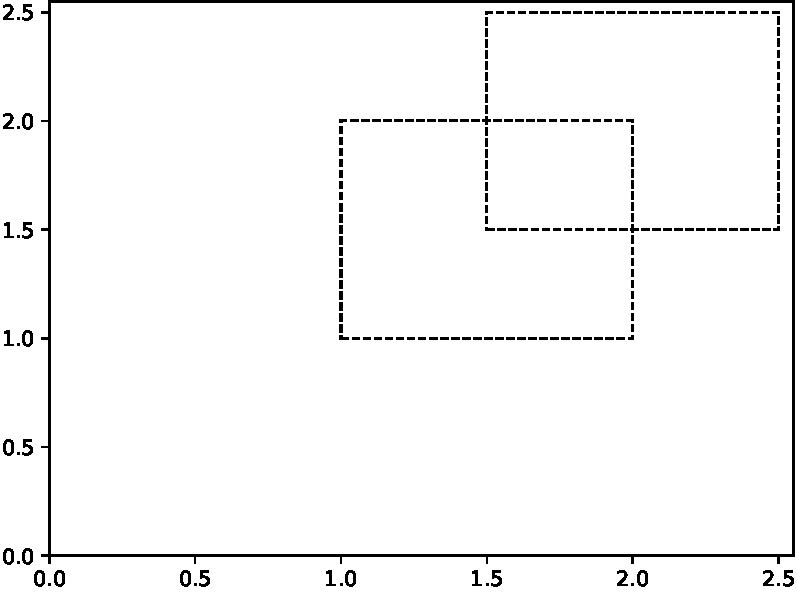
\includegraphics[width=0.6\textwidth]{scripts/rectangles.pdf}
			\end{figure}
			
			Mathematically, we can describe these two rectangles as $(1, 2) \times (1, 2)$ and $(1.5, 2.5) \times (1.5, 2.5)$, and we consider $X = Y = \mathbb R$ with the standard topology.
		\end{remark}
	
		\begin{defn}[Product topology \cite{topology-singh}]
			Let $\mathscr B$ be defined as in Eq. \ref{eq:basis_product_topology}, then $\mathscr B$ fulfills the requirements of Theorem \ref{thrm:gen_top_by_coll_subsets}, and thus $\mathscr B$ generates a topology $\tau(\mathscr B)$ on $X\times Y$, called the \textit{product topology}. When $X \times Y$ is equipped with the product topology, it is also called the \textit{product space}; $X$ and $Y$ are called the \textit{coordinate spaces}. The maps
			\begin{equation}
				\begin{aligned}
					p_X: X\times Y\to X, (x, y) &\mapsto x, \label{eq:projections_coord_spaces} 
					\\ p_Y: X\times Y\to Y, (x, y)&\mapsto y
				\end{aligned}
			\end{equation}
			are projections of the product space $X\times Y$ onto the coordinates spaces.
		\end{defn}
	
		\begin{theorem}
			Let $(X, \tau_X)$ and $(Y, \tau_Y)$ be topological spaces. The projections $p_X$ and $p_Y$ from the product space onto the coordinates spaces, cf. Eq. \eqref{eq:projections_coord_spaces}, are continuous, the product topology is the smallest topology for which this is true, and $p_X$ and $p_Y$ are open maps.
		\end{theorem}
	
		\begin{proof}
			Let $U\in \tau_X$, then $$p_X^{-1}(U) = \left\{(x, y)\in X\times Y \mid p_X((x, y))\in U\right\} = \left\{(x, y)\in X\times Y \mid x\in U\right\} = U\times Y,$$ and thus $p_X$ is continuous in the product topology on $X\times Y$, cf. Definition \ref{defn:continuity_topological_spaces}. Similarly, we can show the continuity of $p_Y$.
			
			Now suppose there is a topology $\mathscr T$ on $X\times Y$ s.t. both $p_X$ and $p_Y$ are continuous. Let $U\in \tau_X$ and $V\in\tau_Y$, then $p_X^{-1}(U) = U\times Y\in \mathscr T$, $p_Y^{-1}(V) = X\times V\in \mathscr T$, and thus
			$$p_X^{-1}(U) \cap p_Y^{-1}(V) = (U\times Y)\cap (X\times V) = (U\cap X) \times (Y\cap V) = U\times V,$$ i.e. all basis elements of the product topology on $X\times Y$ are contained in $\mathscr T$ (note that $\mathscr T$ is a basis for itself, generating $\mathscr T$, cf. Remark \ref{remark:topology_generated_by_topology}), and thus by Theorem \ref{thrm:comp_topologies_bases}, $\mathscr T$ is finer than the product topology on $X\times Y$, i.e. the product topology is the smallest topology on which $p_X$ and $p_Y$ are continuous.
			
			Finally, note that $p_X$ and $p_Y$ are open maps. To see this, note that if $U\in\tau_X$ and $V\in\tau_Y$, then $U\times V$ is open in the product topology, and $p_X(U\times V) = U\in\tau_X$ and $p_Y(U\times V) = V\in\tau_Y$.
		\end{proof}
		
		\begin{defn}[Neighborhood \cite{topology-singh}]
			Let $(X, \tau)$ be a topological space and $x\in X$, then a set $N\subset X$ is called a \textit{neighborhood} of $x$ in $X$ if there is an open set $U\in\tau$ with $x\in U\subset N$.
		\end{defn}
		
		\begin{defn}
			Let $(X, \tau)$ be a topological space, then a sequence $\seq[\varphi_n]$ is said to converge to a point $\varphi\in X$ if for each neighborhood $U$ of $x$, there exists an $N\in\mathbb N$ s.t. for all $n\geq N$, we have $\varphi_n\in U$ \cite{289740}.
		\end{defn}
		
		\begin{remark}
			Unlike metric spaces, the limit point of a converging sequence in topological spaces is not guaranteed to be unique.
		\end{remark}
		
		\begin{exmp}
			Consider $X = \mathbb R$ and the topology $\tau = \left\{\mathbb R, \emptyset\right\}$. Then a sequence $\seq[\varphi_n]$ in $\mathbb R$ converges to any point in $\mathbb R$, since the neighborhood of any $x\in \mathbb R$ is $\mathbb R$.
		\end{exmp}
		
		\begin{defn}[Hausdorff]
			A topology $\left(M, \tau\right)$ is called \textbf{Hausdorff} if $\forall p\ne q \in M \ \exists U$, $V\in \tau$ open with $p\in U$, $q\in V$ such that $U\cap V = \emptyset$.  
		\end{defn} 
		
		\begin{lemma}
			All metric spaces are Hausdorff spaces. 
		\end{lemma}
		
		\begin{proof}
			\begin{figure}[h!]		
				\centering 
				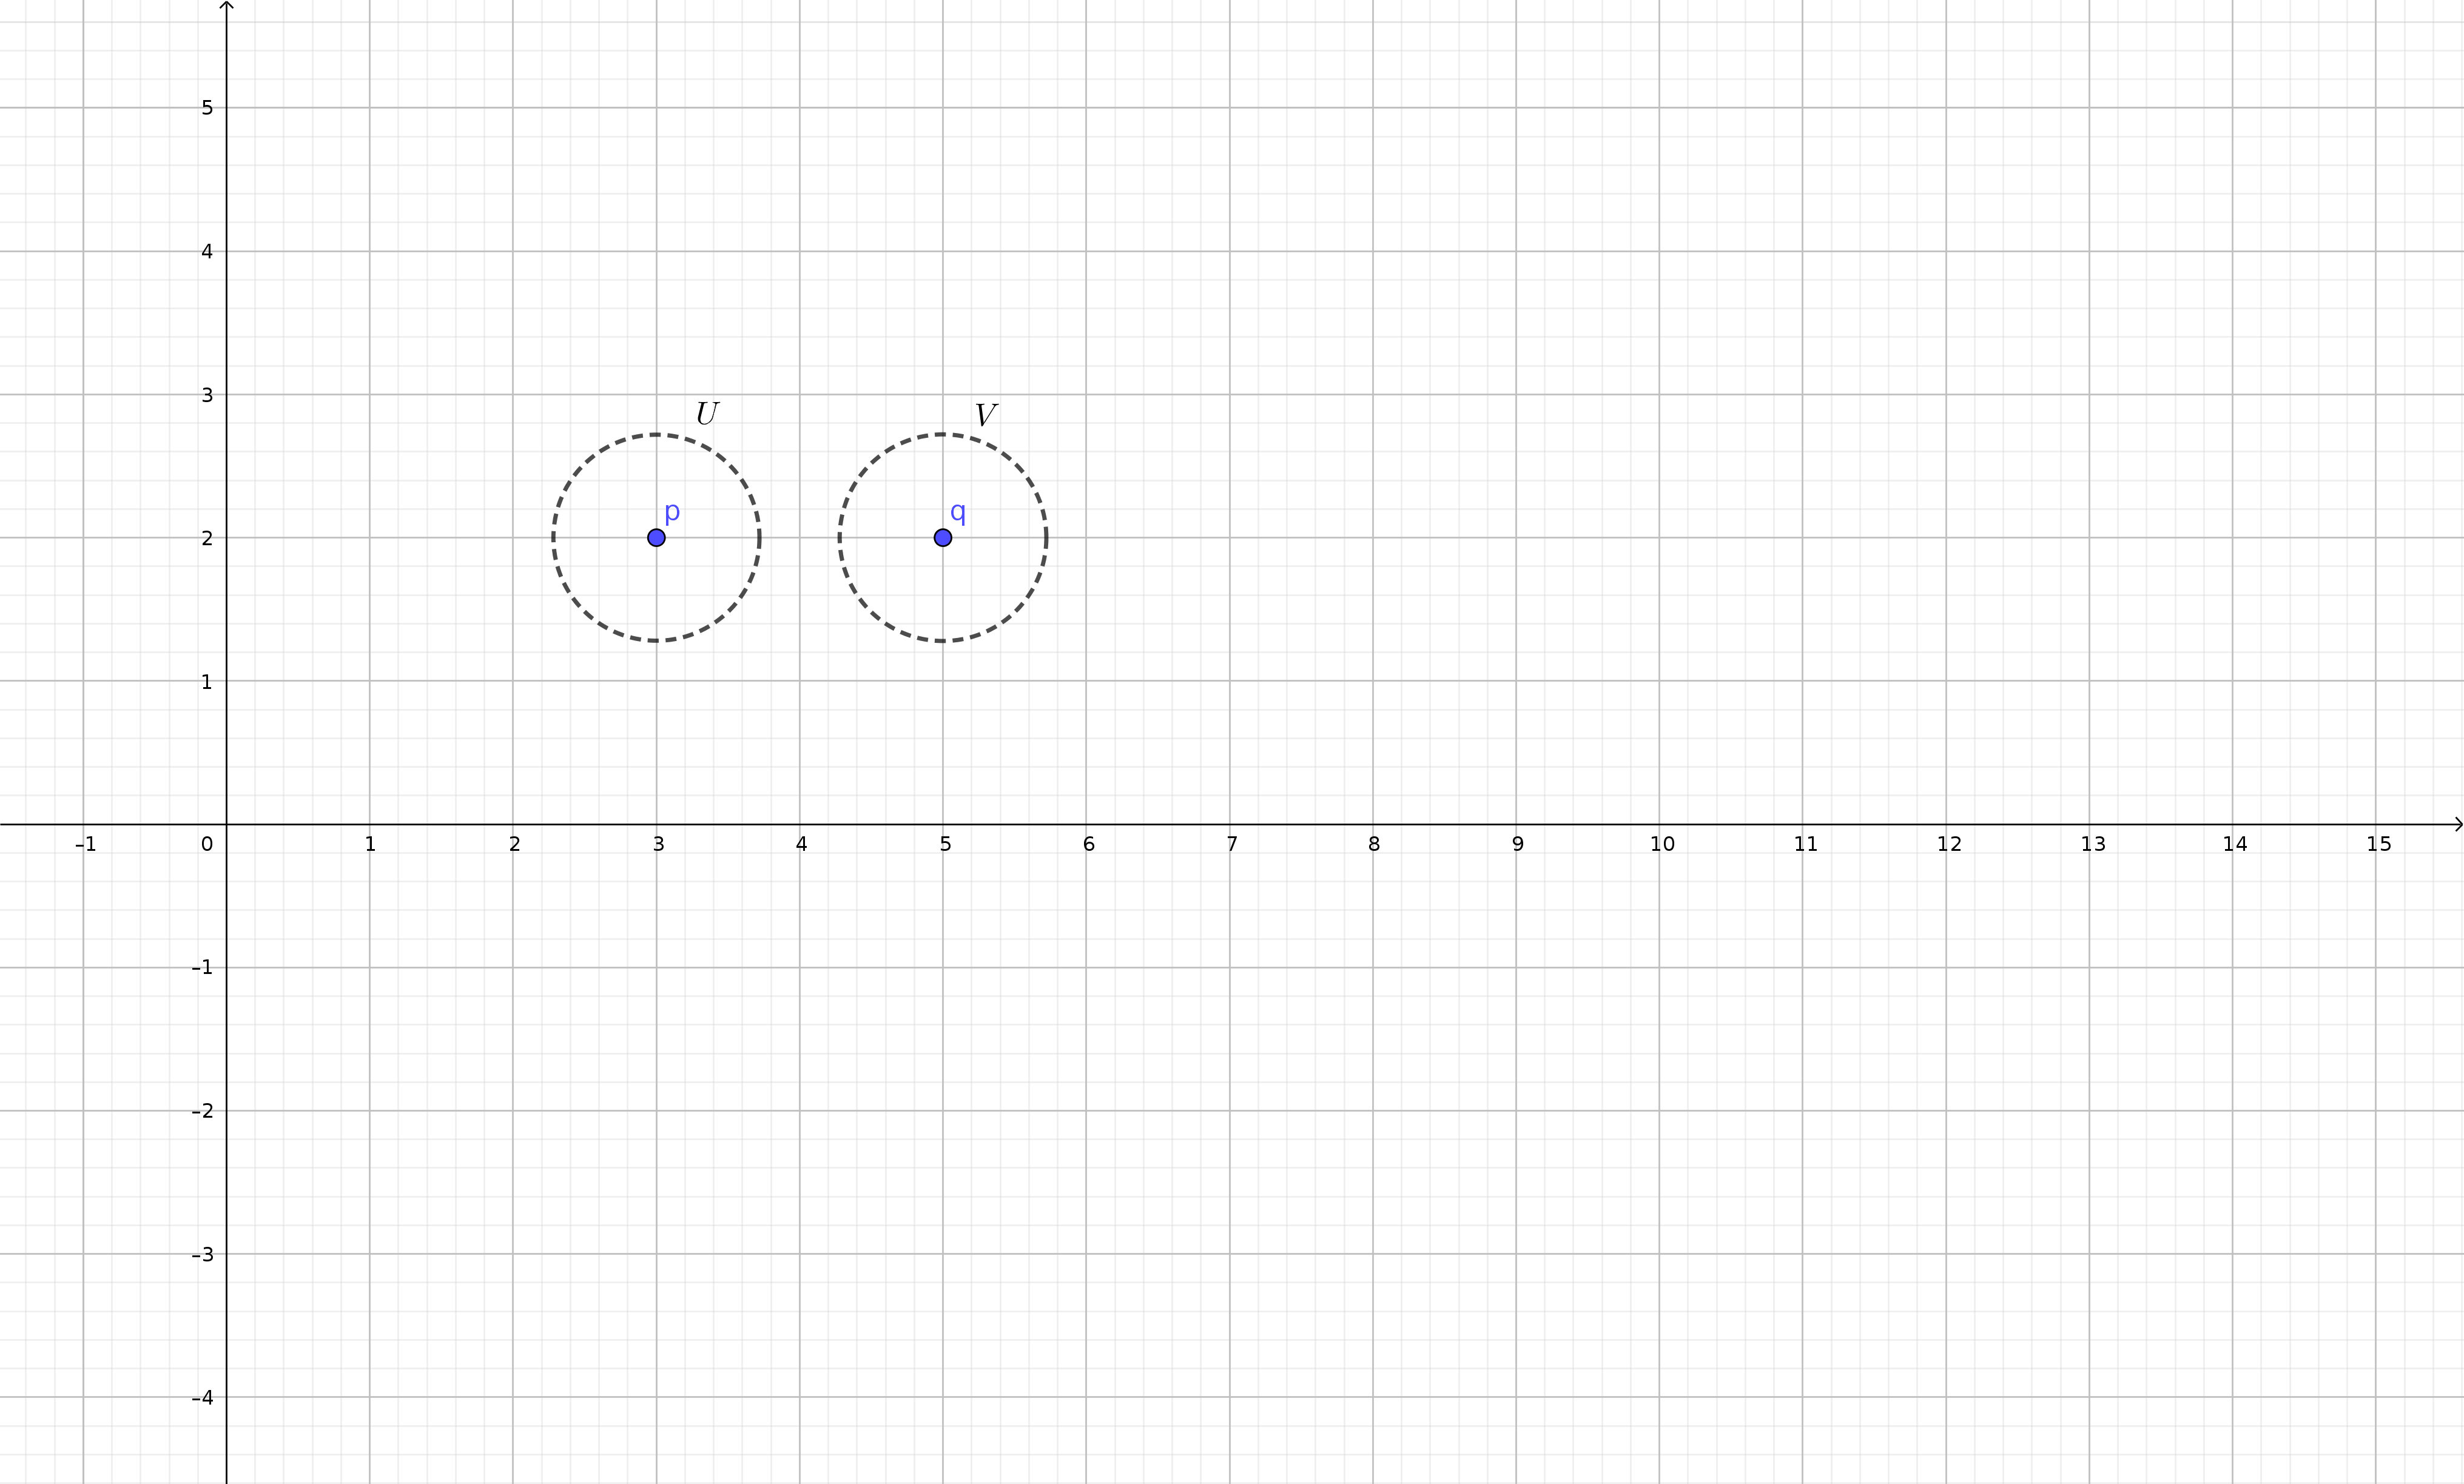
\includegraphics[trim = {3.8cm 5.8cm 9.7cm 2.8cm}, width=0.5\textwidth, clip]{Figures/metric-spaces-Hausdorff-spaces-v2.png}
				\caption{Visualization for why a metric space is a Hausdorff space.}
				\label{metric-space-Hausdorff-space}
			\end{figure} 
			A visualization is shown in Fig. \ref{metric-space-Hausdorff-space}. To prove this more rigorously, define $U := B_{r}(p)$ and $V:=B_{r}(q)$ with radius $r := \frac{d(p, q)}{2}$, where from Theorem \ref{open-balls-open} we know that $U$ and $V$ are open. Suppose $U\cap V = \emptyset$ would not hold. Then there exists a $z\in U\cap V$ with 
			\begin{align}
				d(p, z) < \frac{d(p, q)}{2}
			\end{align}
			and 
			\begin{align}
				d(q, z) < \frac{d(p, q)}{2}. 
			\end{align}
			Therefore, by the triangle inequality for metric spaces, we have: 
			\begin{align}
				d(p, q) \leq d(p, z) + d(q, z) < d(p, q), 
			\end{align}
			which is clearly a contradiction. 
		\end{proof}
		
		\begin{defn}
			Let $(X, \tau)$ be a topological space. Then it is said to be \textit{second countable} if $\tau$ has a countable basis. 
		\end{defn}
		
		\begin{exmp}
			For any $n > 0$, the topological spaces $\mathbb R^n$ are second countable. 
		\end{exmp}
		
		\begin{remark}
			Metric spaces are not automatically second countable. For example, take an uncountable set $X$, endow it with the discrete metric and because of Example \ref{exmp:basis_discrete_metric}, \ref{exmp:metric_topology},  the topological space $X$ is not second countable, since $X$ is uncountable. 
		\end{remark}	
	
		In topological spaces (which are not necessarily metrizable), we define continuity as follows \cite{topology-singh}:
		
		\begin{defn}\label{defn:continuity_topological_spaces}
			Let $(X, \tau_X)$ and $(Y, \tau_Y)$ be topological spaces. Then a function $f: X \to Y$ is called continuous on $X$ if for every $U\in \tau_Y$, $f^{-1}(U) := \{ x\in X \mid f(x)\in U \} \in \tau_X$.
		\end{defn}
		
		\begin{remark}
			In other words, the preimage of an open set is always open. For topological spaces that are metrizable, the $\epsilon$-$\delta$ definition of continuity as in Def. \ref{defn:continuity} is equivalent to the preceding definition, cf. Theorem \ref{thrm:preimages_continuous_functions}.
		\end{remark}
	
		\begin{defn}[Homeomorphism] A \textit{homeomorphism} between two topological spaces $X$ and $Y$ is an invertible function $f: X\rightarrow Y$ such that $f$ and $f^{-1}$ are continuous \cite[p. 33]{topology-singh}. 
		\end{defn}
		
		\begin{exmp}
			The Euclidean space $\mathbb R^n$, equipped with the usual topology, is homeomorphic to the open ball $B_{r}(\varphi) =  \{x\in\mathbb R^n \mid \lvert\lvert x-\varphi \rvert\rvert < r \} \subset \mathbb R^n$ (consider the open ball as a metric space with the \textit{induced metric} from the whole space of $\mathbb R^n$ and then equip it with the usual topology on a metric space given by the open sets). 
		\end{exmp}
		
		\begin{proof}
			Consider the map $$f: \mathbb R^n\rightarrow B_r(\varphi), \ x\mapsto \frac{r\cdot (x-\varphi)}{1+\lvert\lvert x-\varphi\rvert\rvert}.$$ Obviously, $f$ is continuous with inverse $$f^{-1}: B_r(\varphi)\rightarrow \mathbb R^n, \ x \mapsto \frac{x}{r-\lvert\lvert x\rvert\rvert}+\varphi,$$ which is also continuous. One can easily show that $f$ and $f^{-1}$ are inverses to each other. Thus, $f$ describes a homeomorphism. 	
		\end{proof}
				
		\begin{exmp}[Stereographic projection]
			The unit sphere $S^n$, embedded in $\mathbb R^{n+1}$, without the north pole, i.e. $S^n\backslash \{p\} \subset \mathbb R^{n+1}$, where $S^n := \{ x\in\mathbb R^{n+1} \mid \norm{x}{2} = 1 \}$ and $p := \{ x\in\mathbb R^{n+1} \mid x_i = 0 \ \forall i\in[1, n], x_{n+1} = 1 \}$, is homeomorphic to $\mathbb R^n$ (consider the unit sphere as a metric space with the \textit{induced metric} from the whole space of $\mathbb R^{n+1}$ and then equip it with the usual topology on a metric space given by the open sets). 
		\end{exmp}
		\begin{proof}
			Consider the map 
			\begin{align}
				f: S^n\backslash\{p\}\rightarrow \mathbb R^n, \ x\mapsto \frac{1}{1-x_{n+1}}\begin{pmatrix} x_1, \dots, x_n \end{pmatrix}^T. 
			\end{align}
			Obviously, $f$ is continuous. Its inverse is given by 
			\begin{align}\label{stereographic_map_inverse}
				f^{-1}: \mathbb R^n \rightarrow S^n\backslash\{p\}, \ x\mapsto \begin{pmatrix} 2x_1/ \left(1+\norm{x}{2}^2\right)\\ \vdots\\ 2x_n/\left(1+\norm{x}{2}^2\right) \\[4pt] 1-2/\left(1+\norm{x}{2}^2\right) \end{pmatrix}.  
			\end{align}
			It is trivial to show that $f$ and $f^{-1}$ are inverses to each other. One can also easily show that $\norm{f^{-1}(x)}{2} = 1$; thus, $f^{-1}$ does indeed bring us to the unit ball $S^n$. 
			To see that $f^{-1}$ is continuous, note that all components are continuous and thus, according to Lemma \ref{continuity_vector_components}, the function itself is continuous. 
		\end{proof} 
			
	\newpage 
	\section{Linear Functional Analysis}

	\subsection{Bounded Linear Operators}

	Let us start by defining the notions of \textit{linearity} and \textit{boundedness} of operators (\mbox{functionals}). 
	
	\begin{defn}\label{defn:linearity_operator}
		Let $X$, $Y$ be normed linear spaces. Then an operator 
		$A:X\to Y$ is called \textit{linear} if 
		\begin{align}
			A(\alpha \varphi + \beta \psi) = \alpha A(\varphi) + \beta A(\psi) \quad \forall \varphi, \psi\in X, \forall \alpha, \beta\in \mathbb K.
		\end{align}
	\end{defn}

	\begin{theorem}
		A linear operator $A: X\to Y$ from a normed linear space $(X, \norm{\cdot}{X})$ into another normed linear space $(Y, \norm{\cdot}{Y})$ is continuous on $X$ iff it is continuous at a single point in $X$.
	\end{theorem}

	\begin{proof}
		\enquote{$\Longrightarrow$} By definition. 
		
		\enquote{$\Longleftarrow$} Let $A$ be continuous at $\varphi_0\in X$, and let $\seq[\varphi_n]\subset X$ converge to $\varphi\in X$ wrt $\norm{\cdot}{X}$, then
		\begin{align}
			A(\varphi_n) = A(\varphi_n + \varphi_0 - \varphi) - A(\varphi_0 - \varphi) \overset{n\to\infty}{\longrightarrow} A(\varphi)
		\end{align} 
		wrt $\norm{\cdot}{Y}$.
	\end{proof}
	
	\begin{defn}\label{defn:boundedness_operator}
		Let $\left(X, \norm{\cdot}{X}\right)$ and $(Y, \norm{\cdot}{Y})$ be normed linear spaces. Then an operator $A: X\to Y$ is called \textit{bounded} if there is a constant $C(A) > 0$ s.t. 
		\begin{align}
			\norm{A\varphi}{Y} \leq C \norm{\varphi}{X} \quad\forall \varphi\in X.
		\end{align}
		Any such constant $C$ is called an \textit{upper bound} for $A$.
	\end{defn}

	\begin{theorem}
		A linear operator $A: X\to Y$ between normed spaces $(X, \norm{\cdot}{X})$ and $(Y, \norm{\cdot}{Y})$ is bounded iff the operator norm
		\begin{align}
			\norm{A}{} := \sup_{\norm{\varphi}{X} = 1}\norm{A\varphi}{Y} = \sup_{\varphi\in X\backslash \{0\}}\frac{\norm{A\varphi}{Y}}{\norm{\varphi}{X}}
		\end{align}
		on the linear space $\mathcal L(X, Y)$ of all bounded linear operators between the two normed spaces $(X, \norm{\cdot}{X})$ and $(Y, \norm{\cdot}{Y})$ is finite, i.e. 
		\begin{align}
			\norm{A}{} < \infty. 
		\end{align} 
		The operator norm is the smallest upper bound for $A$.
	\end{theorem}
	
	\begin{proof}
		First, let us prove that the operator norm does indeed define a norm on $\mathcal L(X, Y)$. Note that the sum of two operators $A, B\in\mathcal L(X, Y)$ is defined pointwise, i.e. for $\varphi\in X$: $\left(A + B\right)(\varphi) := A\varphi + B\varphi$. Similarly, scalar multiplication is defined for $\alpha \in \mathbb K$ as $\left(\alpha A\right)(\varphi) := \alpha A\varphi$.
		
		The positivity, definiteness and homogeneity of $\norm{A}{}$ are trivial to show. For the triangle equality, note that for any $A, B\in\mathcal L(X, Y)$, we have
		\begin{align}
			\norm{A + B}{} &= \sup_{\norm{\varphi}{X} = 1}\norm{\left(A + B\right)(\varphi)}{Y} = \sup_{\norm{\varphi}{X} = 1}\norm{A\varphi + B\varphi}{Y}
			\\ &\leq \sup_{\norm{\varphi}{X} = 1} \left\{\norm{A\varphi}{Y} + \norm{B\varphi}{Y}\right\} 
			\\ &\leq \sup_{\norm{\varphi}{X} = 1}\{ \norm{A\varphi}{Y} \} + \sup_{\norm{\varphi}{X} = 1}\{ \norm{B\varphi}{Y} \} 
			\\ &= \norm{A}{} + \norm{B}{}.
		\end{align}
	
		Now to the statement $A$ bounded iff $\norm{A}{} < \infty$.
		
		\enquote{$\Longrightarrow$} Let $A$ be upper bounded with bound $C > 0$, then
		\begin{align}
			\norm{A}{} = \sup_{\norm{\varphi}{X} = 1}\norm{A\varphi}{Y} \leq C < \infty.
		\end{align}
		This also shows that $\norm{A}{}$ is the smallest upper bound for $A$.
		\\
		
		\enquote{$\Longleftarrow$} We have 
		\begin{align}
			\norm{A}{} \norm{\varphi}{X} = \sup_{\varphi\in X\backslash \{0\}}\frac{\norm{A\varphi}{Y}}{\norm{\varphi}{X}} \norm{\varphi}{X} = \sup_{\varphi\in X\backslash \{0\}}\norm{A\varphi}{Y} \geq \norm{A\varphi}{Y},
		\end{align}
		which shows that $A$ is bounded with upper bound $C = \norm{A}{} < \infty$ (note that for $v = 0$, there is nothing to show).
	\end{proof}

	\begin{theorem}\label{thrm:continuous-operator-bounded}
		A linear operator $A:X\to Y$ for normed linear spaces $\left(X, \norm{\cdot}{X}\right)$ and $\left( Y, \norm{\cdot}{Y}\right)$ is continuous iff it is bounded.
	\end{theorem}

	\begin{proof}
		\enquote{$\Longleftarrow$} Since $A$ is bounded, by definition, we know that for all $\varphi\in X$, there is an upper bound $C > 0$ s.t. 
		\begin{align}
			\norm{A\varphi}{Y} \leq C\cdot \norm{\varphi}{X}.
		\end{align}
		For an arbitrary $\epsilon > 0$, choose $\delta := \epsilon/C$, then for $\norm{\varphi - \psi}{X} < \delta = \epsilon/C$ (where $\psi\in X$ is arbitary) we have because of the linearity of $A$
		\begin{align}
			\norm{A\varphi - A\psi}{Y} = \norm{A(\varphi - \psi)}{Y} \leq C\norm{\varphi - \psi}{X} < \epsilon,
		\end{align}
		which proves the continuity of $A$, cf. Def. \ref{defn:continuity} \cite{556667}.
		\\
		
		\enquote{$\Longrightarrow$} Let $A$ be continuous on $X$. Then by Theorem \ref{thrm:preimages_continuous_functions}, we know that $A^{-1}\left(B^{Y}_1(0)\right)$ is open, since $B^{Y}_{1}(0)$ is open. By the linearity of $A$, $0\in A^{-1}\left(B^{Y}_1(0)\right)$, since \\ $A(0) = 0 \in B_1^{Y}(0)$. This means that there is an $r > 0$ s.t. $B^{V}_{r}(0) \subset A^{-1}\left(B^{Y}_1(0)\right)$, i.e. the image of $B^{V}_{r}(0)$ is contained in $B^{Y}_{1}(0)$.
		
		Now, for any $a > 1$, choose $C := a/r$, and we will show that $C$ is an upper bound for $A$. For $\varphi\in X\backslash \{0\}$ (for $\varphi =0$, there is nothing to show), note that $$\norm{\frac{r}{a\norm{\varphi}{X}}\varphi}{X} = \frac{r}{a} < r,$$ i.e. 
		\begin{align}
			\frac{r}{a\norm{\varphi}{X}}\varphi \in B_{r}^{V}(0) &\Rightarrow A\left(\frac{r}{a\norm{\varphi}{X}}\varphi\right) = \frac{r}{a\norm{\varphi}{X}}A\varphi\in B^{Y}_{1}(0) 
			\\[6pt] &\Rightarrow \norm{\frac{r}{a\norm{\varphi}{X}}A\varphi}{Y} < 1 \Rightarrow \norm{A\varphi}{Y} \leq \frac{a}{r}\norm{\varphi}{X} = C\norm{\varphi}{X},
		\end{align}
		which completes the proof \cite[p. 2]{src:mit_lec}.
	\end{proof}
	
	\newpage 
	\section{Set Theory}
	\begin{defn}[Binary Relation \cite{binary_relations}]
		A \textit{binary relation} over a set $X$ is some relation $R$ where for all $x$, $y\in X$ the statement $xRy$ is either true or false. 
	\end{defn}
	
	\begin{defn}[Equivalence Relation and Class \cite{equivalence_relation}]\label{defn:equivalence_relation}
		An \textit{equivalence relation} on a set $X$ is a binary relation $\sim$ with the following properties $\forall x$, $y$, $z \in X$: 
		\begin{itemize}
			\item \textbf{reflexivity}: $x\sim x$, 
			\item \textbf{symmetry}: $x \sim y\Leftrightarrow y\sim x$, 
			\item  \textbf{transitivity}: $\left(x\sim y\right) \wedge \left(y\sim z\right)\Rightarrow x\sim z$.  
		\end{itemize}
	\end{defn}

	\begin{defn}[Equivalence Class]
		Let $\sim$ be an equivalence relation on $X$. Then the \textit{equivalence class} of an element $x\in X$ is defined as 
		\begin{align}
			\left[x\right] := \left\{y\in X \mid x\sim y \right\} = \left\{ y\in X \mid y\sim x \right\} \subset X. 
		\end{align}
	
		The set of all equivalences classes in $X$ wrt an equivalence relation $\sim$ is denoted by $X/\sim$. Note that $X/\sim\ \subset P(X)$, where $\mathcal P(X)$ denotes the power set of $X$ \cite{src:quotient_set_X_by_equivalence_relation}. The surjective map $f: X\rightarrow X/\sim, x\mapsto [x]$ is called the \textit{canoninal surjection}.
	\end{defn}

	\begin{theorem}\label{thrm:characterization_equivalence_classes}
		Let $\sim$ be an equivalence relation on $X$. For any $x, y\in X$, it holds that $[x] = [y]$ iff $x\sim y$.
	\end{theorem}
	
	\begin{proof}
		\enquote{$\Longrightarrow$} Since $x\in[x] = [y]$ we have $x\sim y$.
		\\ \\
		\enquote{$\Longleftarrow$} Let $x\sim y$ for arbitrary $x, y\in X$ hold, and consider $x'\in [x]$, i.e. $x'\sim x$. By transitivity, we have $x' \sim y$, i.e. $[x] \subset [y]$. Similarly, we show $[y]\subset [x]$, and hence $[x] = [y]$.
	\end{proof}

	\begin{theorem}
		Let $\sim$ be an equivalence relation on $X$. Then for $x, y\in X$, we either have $[x] \cap [y] = \emptyset$ or $[x] = [y]$.
	\end{theorem}

	\begin{proof}
		We know that the statement $x\sim y$ is either true or false. If it is true, then by Theorem \ref{thrm:characterization_equivalence_classes}, $[x] = [y]$. If $x\not\sim y$, then no $x'\in [x] = \{z\in X\mid x\sim z\}$ can lie in $[y] = \{z'\in X\mid x\sim z'\}$ (and vice versa), because otherwise, by transitivity, $x\sim y$, which we said is false. Hence, $[x] \cap [y] = \emptyset$.
	\end{proof}

	\begin{defn}
		Every element of an equivalence class characterizes it, and can be used to \textit{represent} it. Such a chosen element is called a \textit{representative}.
	\end{defn}

	\begin{defn}[Partially Ordered Set \cite{kuratowski_zorn_lemma}]\label{partially_ordered_set}
		A \textit{partially ordered set}  $\left(X, \leq\right)$ is a set $X$, equipped with a binary relation $\leq$, that satisfies the following properties $\forall x$, $y$, $z\in X$:
		\begin{itemize}
			\item \textbf{reflexivity}: $x\leq x$, 
			\item \textbf{antisymmetry}: $\left(x\leq y\right) \wedge \left(y\leq x\right) \Rightarrow x = y$, 
			\item \textbf{transitivity}: $\left(x\leq y\right) \wedge \left(y\leq z\right)\Rightarrow x\leq z$. 
		\end{itemize}
	\end{defn}

	\begin{defn}[Incomparability]
		In Definition \ref{partially_ordered_set}, the phrasing \enquote{partially ordered} is used to emphasize that there might exist elements $x$, $y\in X$ s.t. both $x\leq y$ and $y\leq x$ are wrong. These pairs are called \textit{incomparable}. If either $x\leq y$ or $y \leq x$ is true, then we say that the pair is \textit{comparable}. 
	\end{defn}
	
	\begin{exmp}
		Consider $X := \left\{\{1\}, \{2\}, \{1, 2\}\right\}$ with $\subset$ as partial ordering. Obviously, the elements $\{1\}$ and $\{2\}$ are incomparable. 
	\end{exmp}

	\begin{defn}[Chain, Upper Bound, Maximal Element]
	For preparing the Kuratowski-Zorn lemma, the following definitions come in handy: 
		\begin{enumerate}[label=\alph*)]
			\item A \textit{chain} $C$ is a partially ordered set where every pair of elements in $C$ is comparable.\ One might also say that $C$ is a \textit{totally ordered set}. 
			\item An \textit{upper bound} (if existent)  of a subset $S\subset X$, where $X$ is a partially ordered set, is an element $u\in X$ such that 
			\begin{align}
				s \leq u \ \forall s\in S. 
			\end{align}
			Since $S\subset X$, $S$ itself is a partially ordered set. 
			\item A \textit{maximal element} (if existent) of a partially ordered set $X$ is an element $m\in X$ such that 
			\begin{align}
				\text{if}\ m\leq x \ \text{for some}\ x\in X,\ \text{then}\ x=m.
			\end{align}
			This is equivalent to saying that there is no $x\in X$ such that $m\leq x$ and $x\ne m$. 
		\end{enumerate}
	\end{defn}

	\begin{remark}
		For an arbitrary partially ordered set $X$, a maximal element (if existent) does not have to be unique.\ For example, consider $X := \left\{ \{1\}, \{2\}, \{3\}, \{1, 2\} \right\}$ with $\subset$ as partial ordering. Both $\{3\}$ and $\{1, 2\}$ are maximal elements.\ However, if we consider chains, then maximal elements are indeed unique by definition. 
	\end{remark}

	\begin{theorem}[Kuratowski-Zorn Lemma]
		Let $\left(M, \leq\right)$ be a non-empty partially ordered set.\ If every chain $C\subset M$ has an upper bound, then $M$ has a maximal element. 
	\end{theorem}

	\begin{remark}
		The upper bound of every chain $C\subset M$ need not be in $C$, by definition of a chain, but it must be in $M$. 
	\end{remark}

	\begin{theorem}[Distributive law for set operations \cite{481036}]
		Let $B$ be a set, and $\{A_i\}$ be a collection of sets, where $I$ is a (finite, countable or uncountable) index set. Then we have
		\begin{align}\label{eq:dist_law_set_ops}
			\left(\bigcup_{i\in I} A_i\right) \cap B = \bigcup_{i\in I}(A_i \cap B)
		\end{align}
		and 
		\begin{align}\label{eq:dist_law_set_ops_2}
			\left(\bigcap_{i\in I}A_i\right) \cup B = \bigcap_{i\in I}(A_i \cup B).
		\end{align}
	\end{theorem}

	\begin{proof}
		We will only show Eq. \eqref{eq:dist_law_set_ops}, since the proof of \eqref{eq:dist_law_set_ops_2} is similar.
		
		If 
		\begin{align*}
			x&\in \left(\bigcup_{i\in I} A_i\right) \cap B \Rightarrow \left(x\in \bigcup_{i\in I}A_i\right) \wedge \left(x\in B\right)\Rightarrow (\exists j\in I: x\in A_j) \wedge (x\in B)
			\\ \Rightarrow x&\in A_j\cap B \subset \bigcup_{i\in I}(A_i \cap B),
		\end{align*}
		i.e. $$\left(\bigcup_{i\in I} A_i\right) \cap B \subset \bigcup_{i\in I}(A_i \cap B).$$
		Conversely, if 
		\begin{align*}
			x&\in \bigcup_{i\in I}(A_i \cap B) \Rightarrow \exists j\in I: x\in A_j \cap B\Rightarrow \left(x\in A_j\subset \bigcup_{i\in I}A_i\right) \wedge \left(x\in B\right)
			\\ \Rightarrow x &\in \left(\bigcup_{i\in I}A_i\right) \cap B,
		\end{align*}
		i.e. 
		$$\bigcup_{i\in I}(A_i \cap B) \subset \left(\bigcup_{i\in I} A_i\right) \cap B,$$
		which completes the proof.
	\end{proof}

	\begin{theorem}\label{thrm:union_of_union_of_sets}
		Let $I$ be an index set, and for each $i\in I$, $J_i$ shall be an index set as well. Then we have \cite{878108}
		\begin{align}
			\bigcup_{i\in I}\left(\bigcup_{j\in J_i}A_j\right) = \bigcup_{j\in\bigcup_{i\in I}J_i}A_j.
		\end{align}		
	\end{theorem}

	\begin{proof}
		\enquote{$\subset$} Let $a\in \bigcup_{i\in I}\left(\bigcup_{j\in J_i}A_j\right)$, i.e. there exists a $i_0\in I$ s.t. $$a\in \bigcup_{j\in J_{i_0}}A_j\subset \bigcup_{j\in \bigcup_{i\in I}J_i}A_j.$$ 
		
		\enquote{$\supset$} 
		\begin{align*}
			a&\in \bigcup_{j\in\bigcup_{i\in I}J_i}A_j 
			\\ \Rightarrow \exists j_0&\in \bigcup_{i\in I}J_i: a\in A_{j_0}
			\\ \Rightarrow \exists i_0&\in I: \left(j_0\in J_{i_0}\right) \wedge \left(a\in A_{j_0}\right)
			\\ \Rightarrow a&\in A_{j_0}\subset \bigcup_{i\in I}\left(\bigcup_{j\in J_i}A_j\right)
		\end{align*}
	\end{proof}
	
	\begin{theorem}\label{thrm:finite_intersec_of_union_of_sets}
		Let $I$ be a \textit{finite} index set, i.e. $I = \{1, \dots, n\}$ for some $n\in \mathbb N$, and for each $i\in I$, $J_i$ shall be an index set as well. Then we have
		\begin{align}\label{eq:finite_intersec_of_union_of_sets}
			\bigcap_{i\in I}\left(\bigcup_{j\in J_i}A_j\right) = \bigcup_{f\in J}\left(\bigcap_{i\in I}A_{f_i}\right),
		\end{align}
		where $J := \prod_{i\in I}J_i = J_1\times \dots\times J_n$, i.e. $f\in J$ is an $n$-tuple, and hence $f = (f_1, \dots, f_n)$ with $f_i\in J_i$ for each $i\in I$.
	\end{theorem}
	
	\begin{proof}
		Via induction. For $n = 1$, we have $I = \{1\}$ and $f = f_1\in J_1$, and thus
		$$\bigcap_{i\in I}\left(\bigcup_{j\in J_i}A_j\right) = \bigcup_{j\in J_1} A_j = \bigcup_{f\in J_1}\left(\bigcap_{i\in I}A_{f}\right).$$
		
		For the induction step, note that if Eq. \eqref{eq:finite_intersec_of_union_of_sets} holds for an $n\in\mathbb N$, and we define $I' := \{1, \dots, n, n+1\}$ and $J' := J\times\prod J_{n+1} = \prod_{i\in I'}J_i$, then
		\begin{align*}
			\bigcap_{i\in I'}\left(\bigcup_{j\in J_i}A_j\right) 
			&= \left( \bigcup_{j\in J_1}A_j \right) \cap \dots\cap \left(\bigcup_{j\in J_n}A_j\right)\cap \left(\bigcup_{j\in J_{n+1}}A_j\right) 
			\\ &\overset{\small\text{IA}}{=} \left(\bigcup_{f\in J}\left(\bigcap_{i\in I}A_{f_i}\right)\right) \cap \left(\bigcup_{j\in J_{n+1}}A_j\right) 
			\\ &\overset{\tiny\eqref{eq:dist_law_set_ops}}{=} \bigcup_{f\in J}\left(\left( \bigcap_{i\in I}A_{f_i}\right) \cap \left( \bigcup_{j\in J_{n+1}}A_j \right)\right)
			\\[6pt] &\overset{\tiny\eqref{eq:dist_law_set_ops}}{=} \bigcup_{f\in J}\bigcup_{f_{n+1}\in J_{n+1}} \left( \bigcap_{i\in I'}A_{f_i}\right)
			\\[6pt] &= \bigcup_{f\in J'}\left( \bigcap_{i\in I'}A_{f_i}\right).
		\end{align*}
	\end{proof}
	
	\newpage 
	\section{Differential Geometry}
	\begin{samepage}
		\begin{defn}[Smooth Atlas \cite{Lindemann-lec1}]
			Let $M$ be a second countable Hausdorff topological space. An \textit{$n$-dimensional smooth atlas on $M$}  is a collection of maps
			\begin{align*}
				\mathcal A = \left\{\left(\varphi_i, U_i\right)\mid i\in I\right\}, \quad \varphi_i: U_i \rightarrow \varphi_i(U_i) \subset \mathbb R^n
			\end{align*}
			such that all $U_i \subset M$ are open, all $\varphi_i$ are homeomorphisms, $I$ is an index set and 
			\begin{itemize}
				\item $\{U_i \mid i\in I\}$ is an open covering of $M$, 
				\item $\varphi_i \circ \varphi_j^{-1}: \varphi_j(U_i \cap U_j) \rightarrow \varphi_i(U_i \cap U_j)$ are smooth $\forall i$, $j \in I$. 
			\end{itemize}
			The tuples $(\varphi_i, U_i)$, $i\in I$, are so-called \textit{charts} on $M$, the maps $\varphi_i\circ \varphi_j^{-1}$ are called \textit{transition maps} or \textit{changes of coordinates} and $n$ is the \textit{dimension} of $M$.
		\end{defn}
	\end{samepage}

	\begin{remark}
		To see why the domain of the transition maps $\varphi_i \circ \varphi_j^{-1}$ is $\varphi_j\left(U_i \cap U_j\right)$, note that the expression $\varphi_i\left(\varphi_j^{-1}\left(x\right)\right)$ only makes sense if 
		\begin{align*}
			\left(x\in \varphi_j(U_j)\right) \wedge  \left(\varphi_j^{-1}\left(x\right)\in U_i\right) \Rightarrow \left(x\in \varphi_j(U_j)\right) \wedge \left(x\in \varphi_j\left(U_i\right)\right) \Rightarrow x\in \varphi_j(U_j \cap U_i). 
		\end{align*}
		Similarly, we can convince ourselves that the codomain of the transition maps $\varphi_i\circ\varphi_j^{-1}$ is given by $\varphi_i(U_i\cap U_j)$. Since $x\in \varphi_j(U_j)$, it follows that $\varphi_j^{-1}(x)\in U_j$. In addition, due to the domain of the homeomorphism $\varphi_i$, it must hold that $\varphi_j^{-1}(x) \in U_i$. Thus: 
		\begin{align*}
			\left(\varphi_j^{-1}(x)\in U_j\right) &\wedge \left(\varphi_j^{-1}(x) \in U_i\right) 
			\\
			\Rightarrow 			\left(\varphi_i(\varphi_j^{-1}(x))\in \varphi_i(U_j)\right) &\wedge \left(\varphi_i(\varphi_j^{-1}(x))\in \varphi_i(U_i)\right) 
			\\ 
			\Rightarrow \varphi_i\left(\varphi_j^{-1}(x)\right) &\in \varphi_i\left(U_i\cap U_j\right). 
		\end{align*}
	\end{remark}
	
	\begin{defn}[Equivalence of Atlases]
		Let $M$ be a second countable Hausdorff topological space. Two atlases $\mathcal A$ and $\mathcal B$ on $M$ are called \textit{equivalent} if $\mathcal A\cup \mathcal B$ is an atlas on $M$.  
	\end{defn}

	\begin{remark}
		To see that not all atlases are equivalent to each other, consider $M = \mathbb R$ (which is a second countable Hausdorff topological space). Consider the atlases $\mathcal A = \{ (\varphi, M) \}$ with $\varphi: M\rightarrow M$, $x\mapsto x$ and $\mathcal B = \{(\psi, M)\}$ with $\psi: M\rightarrow M$, $x\mapsto x^3$. The atlases are not equivalent, since $\varphi\circ \psi^{-1}: M \rightarrow M$, $x\mapsto \sqrt[3]{x}$ is not smooth (the derivative is not continuous). 
	\end{remark}
	
	\newpage 
	\section{Normalizing Flows}
	\begin{defn}\label{defn-diffeomorphism}
		Let $M$, $N$ be two manifolds, $g: M\rightarrow N$ a differentiable map. If $g$ is a bijection and its inverse $g^{-1}: N\rightarrow M$ is differentiable as well, then we call $f$ a \textit{diffeomorphism}. We talk of a $C^k$ \textit{diffeomorphism} if both $g$ and $g^{-1}$ are $k$-times continuously differentiable. 
	\end{defn}
	
	\begin{theorem}[Change of variables \cite{MfPIII}]\label{change-of-variables}
		Let $U$, $V\subset\mathbb{R}^n$ be open subsets and $T: U\rightarrow V$ a diffeomorphism, cf. Def.  \ref{defn-diffeomorphism}. Then the function $f: V\rightarrow \mathbb{C} \ \cup \{\infty\}$ is integrable over $V$ if and only if the function 
		\begin{align}
			\left(f\circ T\right) \cdot \left\vert \det \left( \frac{\partial T_{\mu}}{\partial x_{\nu}} \right)_{\mu\nu} \right\vert 
		\end{align}
		is integrable over $U$. In this case, it holds that 
		\begin{align}\label{change-of-variables-formula}
			\int_{U} \left(f\circ T\right)(x) \cdot \left\vert \det\left(\frac{\partial T_{\mu}}{\partial x_{\nu}}(x)\right)_{\mu, \nu} \right\vert dx = \int_{V} f(y)dy. 
		\end{align}
	\end{theorem}
	\begin{remark}\label{diffeomorphism-inverse}
		If $T$ is a diffeomorphism, then also $T^{-1}$ is a diffeomorphism, thus we could also have chosen $T^{-1}$ in the formulation of Theorem \ref{change-of-variables}.
	\end{remark}
	
	\begin{theorem}[Inverse function theorem \cite{IFT}] Let $g: \mathbb R^n \rightarrow \mathbb R^n$ be continuously differentiable on some open set $V\subset \mathbb R^n$ containing $\mathbf{a}$ and suppose $\det Jg(\mathbf{a}) \ne 0$, where $J$ shall be the Jacobi matrix of $g$. Then there is some open set containing $\mathbf{a}$ and an open set $W\subset \mathbb{R}^n$ containing $g(\mathbf{a})$ such that $g: V\rightarrow W$ has a continuous inverse $g^{-1}: W\rightarrow V$ which is differentiable for all $\mathbf{y}\in W$. 
		\\ \\	
		As matrices, we can write this as 
		\begin{align}
			J(g^{-1})(\mathbf{y}) = \left[\left(Jg\right)\left(g^{-1}(\mathbf{y})\right)\right] ^{-1}
		\end{align} 
	\end{theorem}
	
	\begin{remark} An example for a function that is invertible and continuously differentiable but not a diffeomorphism is $g: \mathbb{R}\rightarrow\mathbb{R}$, $x\mapsto x^3$. Its inverse is obviously $g^{-1}: \mathbb{R}\rightarrow\mathbb{R}, x\mapsto \sqrt[3]{x}$, cf. \cite{cube-root} for a nice plot. However, $\frac{dg^{-1}}{dx}|_{x = 0}$ does not exist. The reason is that $\det Jg(0) = 0$ and hence the inverse function theorem does not apply. 
	\end{remark}
	\begin{itemize}
		\item Let $\mathbf{U}$ be a random variable and let $p(\mathbf{U})$ describe the probability distribution of it, e.g. a uniform distribution between $0$ and $1$. We now make a simple transformation and obtain a new random variable $\mathbf{X}$, where we again denote by $p(\mathbf{X})$ the probability distribution of $\mathbf{X}$. We obtain $\mathbf{X}$ in the following way: 
		\begin{align}\label{normalizing-flow-forward}
			p(\mathbf{X}) = p(\mathbf{U})\left\vert \det\left(\frac{\partial\mathbf{f}}{\partial \mathbf{U}}\right)\right\vert^{-1}, 
		\end{align}
		where $\mathbf{f}$ denotes an invertible (and hence bijective) mapping. 
		
		\item Without proof, it holds that 
		\begin{align}
			\left\vert \det\left(\frac{\partial\mathbf{f}}{\partial\mathbf{U}}\right)\right\vert^{-1} = \left\vert \text{det}\left(\frac{\partial\mathbf{f}^{-1}}{\partial\mathbf{U}}\right) \right\vert 
		\end{align}
		and thus we can rewrite Eq. \eqref{normalizing-flow-forward} as 
		\begin{align}\label{normalizing-flow-backward}
			p(\mathbf{U}) = p(\mathbf{X})\left\vert \det\left(\frac{\partial\mathbf{f^{-1}}}{\partial \mathbf{U}}\right)\right\vert^{-1}. 
		\end{align}
		Since we assumed $\mathbf{f}$ to be invertible, $\mathbf{f^{-1}}$ is well-defined. 
		
		\item In practice, we will want $\mathbf{f}$ to be both invertible \underline{and} to have a \textbf{tractable} Jacobian, i.e. a Jacobian that we can easily calculate. For $\mathbf{f}$ to have a Jacobian at all, each of its first-order partial derivatives must exist \cite{jacobi-matrix}.
		So-called \textit{autoregressive flows} have the property that their Jacobian is an \underline{upper triangular matrix}. For an upper triangular matrix, it holds that its determinant is given by the product of its diagonal elements \cite{triangular-matrices}.
	\end{itemize}

	\begin{defn}[Determinant]
		Let $D$ be an $n\times n$ matrix and let $S_n$ denote the symmetric group over $n$. Then the determinant of $D$ is defined as:  
		\begin{align}
			\det(D) := \sum_{\sigma\in S_n} \left( \text{sgn}(\sigma) \prod_{i = 1}^{n}a_{i, \sigma(i)} \right),  
		\end{align}
		cf. \cite{leibniz-formula}. 
	\end{defn}

	\begin{lemma}
		Let $A$ be a $k\times k$, $0$ an $k\times n$, $C$ an $n\times k$ and $D$ an $n\times n$ matrix; then 
		\begin{align}
			\det\left( \begin{pmatrix}	A & 0 \\ C & D \end{pmatrix} \right) = \det(A)\det(D). 
		\end{align}
	\end{lemma}
	
	\begin{proof}
		Define 
		\begin{align}
			B := \begin{pmatrix} A & 0 \\ C & D
			\end{pmatrix}. 
		\end{align}
		Clearly, 
		\begin{align}\label{case-diff}
			b_{i,j} = 
			\begin{cases}
				a_{i, j} \qquad &i, j\leq k, \\
				0 		 \qquad &i\leq k, j \geq k+1, \\
				c_{i-k, j} \qquad &i\geq k+1, j \leq k, \\
				d_{i-k, j-k} \qquad &i, j\geq k+1. 
			\end{cases}
		\end{align}
		We can write the determinant of $B$ as 
		\begin{align}
			\det(B) = \sum_{\sigma\in S_{n+k}} \text{sgn}(\sigma)\prod_{i = 1}^{n+k}b_{i, \sigma(i)}. 
		\end{align}
		From Eq. \eqref{case-diff} we know that all summands of the form $\sigma(i) = j$ with $i\leq k$, $j\geq k+1$ are $0$. Therefore, we can consider all permutations of the form $\sigma(i) = j$ with $i, j \leq k$ or $\sigma(i) = j$ with $i\geq k+1$, $j\leq k$. We can also write this in the form $\sigma(i) = \pi(i)$ for $i\leq k$ and $\sigma(k + i) = k + \tau(i)$ for $1\leq i \leq n$, where $\pi\in S_k$ and $\tau\in S_n$. Denote the set of all such permutations by $\tilde{S}_{k+n}$.  Thus: 
		\begin{align}
			\det(B) &= \sum_{\sigma\in\tilde{S}_{k+n}}\text{sgn}(\sigma)\prod_{i = 1}^{n+k}b_{i, \sigma(i)}
			\\ &= \sum_{\sigma\in\tilde{S}_{k+n}}\text{sgn}(\sigma)\prod_{i = 1}^{k}b_{i, \sigma(i)}\prod_{i = k+1}^{n+k}b_{i, \sigma(i)}
			\\ &\overset{\tiny\eqref{case-diff}}{=} \sum_{\sigma\in\tilde{S}_{k+n}}\text{sgn}(\sigma)\prod_{i = 1}^{k}a_{i, \sigma(i)}\prod_{i=k+1}^{n+k}d_{i-k, \sigma(i)-k}
			\\ &= \sum_{\sigma\in\tilde{S}_{k+n}}\text{sgn}(\sigma)\prod_{i = 1}^{k}a_{i, \sigma(i)}\prod_{i = 1}^{n}d_{i, \sigma(i+k)-k}
			\\ &= \sum_{\pi\in S_k, \tau\in S_n}\text{sgn}(\pi)\text{sgn}(\tau)\prod_{i = 1}^{k}a_{i, \pi(i)}\prod_{i = 1}^{n}d_{i, \tau(i)}
			\\ &= \sum_{\pi\in S_k}\text{sgn}(\pi)\prod_{i = 1}^{k}a_{i, \pi(i)}\sum_{\tau\in S_n}\text{sgn}(\tau)\prod_{i = 1}^{n}d_{i, \tau(i)}
			\\ &= \det(A)\det(D)
		\end{align}
		\cite{block-triangular-matrix}
	\end{proof} 
		
	\begin{defn}
		Let $h(\bm{\cdot}\ ; \theta): \mathbb{R}\rightarrow\mathbb{R}$ be a bijection parametrized by $\theta$. Then an \textit{autoregressive model} is a function \begin{align}
			g: \mathbb{R}^D\rightarrow\mathbb{R}^D, \begin{pmatrix}
				x_1 \\ \dots \\ x_D 
			\end{pmatrix} \mapsto 
			\begin{pmatrix}
				h\left(x_1; \Theta_1\right) \\ h\left(x_2; 	\Theta_2\left(x_1\right)\right) \\ \dots \\ h\left(x_D; \Theta_D\left(x_1, \dots, x_{D-1}\right)\right)
			\end{pmatrix}
		\end{align}
		The functions $\Theta_t$ for $t = 2$, $\dots$, $D$ are arbitrary functions whose domain is $\mathbb{R}^{t-1}$, $\Theta_1$ is a constant. 
	\end{defn}

	\begin{remark}
		The Jacobian matrix of an autoregressive flow is given as follows: 
		\begin{align}
			Dg &= \begin{pmatrix}
				\partial g_1/\partial x_1 & \partial g_1/\partial x_2 & \dots & \partial g_1/\partial x_D 
								\\ 
				\partial g_2/\partial x_1 & \partial g_2/\partial x_2 & \dots & \partial g_2/\partial x_D
								\\
				\vdots & \vdots & \ddots & \vdots 
								\\ 
				\partial g_D/\partial x_1 & \partial g_D / \partial x_2 & \dots & \partial g_D / \partial x_D
			\end{pmatrix} 
		\end{align}
	One can easily convince oneself that $Dg$ is a lower triangular matrix. 
	\end{remark}

	\begin{theorem}
		Normalizing flows in $\mathbb{R}^D$ come from the push-forward of a measure. 
	\end{theorem}
	
	\begin{proof}
		Let $\mathcal Y$, $\mathcal Z\subset\mathbb{R}^D$ be open,  $\Sigma_{\mathcal Y} = \mathcal B(\mathcal Y)$, $\Sigma_{\mathcal Z} = \mathcal B(\mathcal Z)$ and $g: \mathcal Z\rightarrow\mathcal Y$ be a diffeomorphism. The function $g: \mathcal Z \rightarrow \mathcal Y$ is measurable if and only if $g^{-1}(G)\in \Sigma_{\mathcal Z}$ for every set $G$ that is open in $\mathcal Y$, cf. Theorem \ref{generator-and-measurable-function} (Borel $\sigma$-algebras are generated by the open sets). Since for functions between two topological spaces it holds that they are continuous if and only if the inverse image of an open set is again open, we have that $g$ is indeed measurable. 
		\\ \\ Now define the probability measure $\mu$ on the measurable space $(\mathcal Z, \Sigma_{\mathcal Z})$ as 
		\begin{align}\label{prob-measure-proof}
			\mu(I) := \int_{I} p_{\mathbf{Z}}(z)d\lambda(z) \ \forall I\in \Sigma_{\mathcal Z}, 
		\end{align}
		where $p_{\mathbf{Z}}: \mathcal Z \rightarrow\mathbb{R}$ shall be a PDF and $\lambda$ the Lebesgue measure. (The Lebesgue measure is defined on the completion of $\mathcal B(\mathbb R^D)$, which is \enquote{larger} than $\mathcal B(\mathbb R^D)$.) By considering the push-forward of $\mu$ under the measurable map $g$, we have $\forall J \in \Sigma_{\mathcal Y}$: 
		\begin{align}
			g_{\star}\mu\left(J\right) = \mu(g^{-1}(J))  \overset{\tiny\eqref{prob-measure-proof}}{=} \int_{g^{-1}(J)} p_{\mathbf{Z}}(z)d\lambda(z)
		\end{align}
		Since by assumption $g:\mathcal Z\rightarrow \mathcal Y$ and therefore also the inverse $g^{-1}: \mathcal Y \rightarrow \mathcal Z$ are a diffeomorphism, we can use the change of variables formula from Theorem \ref{change-of-variables}, since we assume $p_{\mathbf{Z}}$ to be integrable over $\mathcal Z$. We apply Theorem \ref{change-of-variables} to $g^{-1}$ instead of $g$, cf. Remark \ref{diffeomorphism-inverse}: 
		\begin{align}
			g_{\star}\mu(J) = \int_{g^{-1}(J)}p_{\mathbf{Z}}(z)d\lambda(z) = \int_{J} \underbrace{\left(p_{\mathbf{Z}}\circ g^{-1}\right)(y) \cdot \left\vert \det Dg^{-1}(y) \right\vert }_{= p_{\mathbf{Y}}(y)} d\lambda(y) 						
		\end{align}
	\end{proof}
	
	\begin{defn}
		A rational-quadratic function takes the form of a quotient of two quadratic polynomials. 
		\begin{align}
			\frac{\alpha^{(k)}\left(\xi\right)}{\beta^{(k)}(\xi)} = \frac{a_0\xi^2 + a_1\xi + a_2}{b_0\xi^2 + b_1\xi + b_2} 
		\end{align}
	\end{defn}	

\newpage 

\section{Diffusion-Based Models}
	
	\begin{remark}[ELBO VAEs]
		One can easily show that the (marginal) log-likelihood of the data is given as
		\cite{cs_231n_lec_13}
		\begin{align}\label{eq:elbo__marginal_LL}
			\log p(x) = \text{ELBO} + D_{\text{KL}}\left[ q_{\phi}(z\vert x) \vert\vert p(z\vert x)\right], 
		\end{align}
		
		\noindent where $p(z\vert x)$ is the true posterior and ELBO is the usual evidence lower bound, i.e.
		\begin{align}
			\text{ELBO} = \mathbb E_{q_{\phi}(z\vert x)}\left[ \log p_{\psi}(x\vert z) \right] - D_{\text{KL}}\left[ q_{\phi}(z\vert x) \vert\vert p(z) \right]
		\end{align}
		
		\noindent Eq.~\eqref{eq:elbo__marginal_LL} shows that since the (marginal) log-likelihood is not parameterized by any NN parameters, maximizing the ELBO necessary leads to a lower $D_{\text{KL}}\left[ q_{\phi}(z\vert x) \vert\vert p(z\vert x)\right]$, which is the reverse KLD. 
		
	\end{remark}

\begin{lemma}[ELBO]
	Let $q(x_{0})$ denote the true (unknown) distribution of a real image $x_{0}$, and let $p_{\theta}(x_{0})$ be the model's approximation to $q(x_{0})$, then we have the following ELBO-like loss: 
	\begin{align}\label{elbo_diffusion_models}
		\mathbb E_{q(x_{0})}\left[\log p_{\theta}(x_{0})\right] \geq -\mathbb E_{q(x_{0}, \dots, x_{T})}\left[\log \frac{q(x_{1}, \dots, x_{T} \mid x_{0})}{p_{\theta}(x_{0}, \dots, x_{T})}\right].    
	\end{align}
\end{lemma}

\begin{proof}
\cite{lilian_weng}
	\begin{align}
		\log p_{\theta}(x_{0}) &\geq \log p_{\theta}(x_{0}) - D_{\text{KL}}\left[ q(x_{1}, \dots, x_{T}\mid x_{0})\mid\mid p_{\theta}(x_{1}, \dots, x_{T}\mid x_{0}) \right]
		\\[4pt] &= \log p_{\theta}(x_{0}) - \mathbb E_{q(x_{1}, \dots, x_{T}\mid x_{0})}\left[\log\frac{q(x_{1}, \dots, x_{T}\mid x_{0})}{p_{\theta}(x_{1}, \dots, x_{T} \mid x_{0})}\right]
		\\[4pt] &= \log p_{\theta}(x_{0}) - \mathbb E_{q(x_{1}, \dots, x_{T}\mid x_{0})}\left[\log\frac{q(x_{1}, \dots, x_{T}\mid x_{0})}{p_{\theta}(x_{0}, \dots, x_{T})/ p_{\theta}(x_{0})}\right]
		\\[4pt] &= -\mathbb E_{q(x_{1}, \dots, x_{T}\mid x_{0})}\left[\log\frac{q(x_{1}, \dots, x_{T}\mid x_{0})}{p_{\theta}(x_{0}, \dots, x_{T})}\right]
		\\[4pt] \Rightarrow \mathbb E_{q(x_{0})}\left[\log p_{\theta}(x_{0})\right] &\geq -\mathbb E_{q(x_{0})}\mathbb E_{q(x_{1}, \dots, x_{T}\mid x_{0})}\left[\log\frac{q(x_{1}, \dots, x_{T}\mid x_{0})}{p_{\theta}(x_{0}, \dots, x_{T})}\right]
	\end{align}
	Assuming that the assumptions of Fubini's theorem hold and from the monotonicity of the expectation, we have: 
	\begin{align}\label{diff_elbo_to_be_proved}
		\mathbb E_{q(x_{0})}\left[ \log p_{\theta}(x_{0}) \right] &\geq \mathbb E_{q(x_{1}, \dots,  x_{T} \mid x_{0})q(x_{0})}\left[\log \frac{q(x_{1}, \dots, x_{T} \mid x_{0})}{p_{\theta}(x_{0}, \dots, x_{T})}\right] 
		\\ &= E_{q(x_{0}, \dots,  x_{T} \mid x_{0})}\left[\log \frac{q(x_{1}, \dots, x_{T} \mid x_{0})}{p_{\theta}(x_{0}, \dots, x_{T})}\right].
	\end{align}
\end{proof}

\begin{defn}[Wiener process]
	Let $W_{t}$ be a real-valued continuous-time stochastic process.\ It is said to be a \textit{Wiener process} if the following properties hold: 
	\begin{itemize}
		\item $W_{0} = 0$, 
		\item $W$ has independent increments, i.e.\ $\forall t > 0:$, the terms $W_{t+u} - W_{t}$, $u\geq 0$ are independent of past values $W_{s}$, $s\leq t$, 
		\item $W$ has Gaussian increments:\ $W_{t+u} - W_{t} \sim \mathcal N(0, u)$, 
		\item $W$ has continuous paths, i.e.\ $\forall t$, $W_{t}$ is continuous in $t$. 
	\end{itemize}
	source:\ \url{https://en.wikipedia.org/wiki/Wiener_process}
\end{defn}

\begin{remark}
	If $\xi_{1}$, $\xi_{2}$, $\dots$ be i.i.d random variables with a mean of $0$ and standard deviation of $1$.\ For every $n$, define a continuous time stochastic process 
	\begin{align}\label{random_walk_Wiener}
		W_{n}(t) := \frac{1}{\sqrt{n}}\sum_{1\leq k\leq\lfloor nt \rfloor}\xi_{k} 
	\end{align}
	This is what makes Wiener processes so powerful (and explains the ubiquity of Brownian motion).\ According to Donsker's theorem, the  above expression becomes a Wiener process.
\end{remark}

\newpage 

\section{Miscellaneous}

	\begin{lemma}[Chain rule for KL-divergences]
		Let $p(x, y)$ and $q(x, y)$ be two arbitrary PDF's. Then the following hods:
		
		\begin{align}
			D_{\text{KL}}(p(x, y) \vert\vert q(x, y)) = D_{\text{KL}}(p(x)\vert\vert q(x)) + D_{\text{KL}}(p(y\vert x) \vert\vert q(y\vert x))
		\end{align}
		
		\begin{proof}
			Brute-force calculation yields:
			\begin{align}
				D_{\text{KL}}(p(x, y) \vert\vert q(x, y)) &= \int\int p(x, y)\log\frac{p(x, y)}{q(x, y)}d\lambda(x)d\lambda(y)
				\\[4pt] &= \int\int p(x, y)\log\frac{p(x)p(y\vert x)}{q(x)q(y\vert x)}d\lambda(x)d\lambda(y)
				\\[4pt] &= \int\int p(x, y)\log\frac{p(x)}{q(x)}d\lambda(x)d\lambda(y) + \int\int p(x, y)\log\frac{p(y\vert x)}{q(y\vert x)}d\lambda(x)d\lambda(y)
				\\[4pt] &= D_{\text{KL}}(p(x) \vert\vert q(x)) + \int p(x)d\lambda(x)\int p(y\vert x)\log\frac{p(y\vert x)}{q(y\vert x)}d\lambda(y)
				\\[4pt] &= D_{\text{KL}}(p(x) \vert\vert q(x)) + D_{\text{KL}}(p(y\vert x) \vert\vert q(y\vert x))
			\end{align}
		\end{proof}
	\end{lemma}
	
	\begin{defn}[Mutual information]
		Let $(X, Y)\sim P_{\left(X, Y\right)}\in \mathcal P(\mathcal X\times \mathcal Y)$, where $\mathcal P(\mathcal X\times \mathcal Y)$ is the space of all probability measures over the space $\mathcal X\times \mathcal Y$. The mutual information between the random variables $X$ and $Y$ is now defined as 
		\cite[Def.~10.1]{ece_ece_5630_lectures10}:
		
		\begin{align}
			I(X; Y) := D_{\text{KL}}\left(P_{(X, Y)} \vert\vert P_{X} \otimes P_{Y}\right),
		\end{align}
	
		\noindent where $P_{X}$ and $P_{Y}$ are the marginal measures of the coupling measure $P_{(X, Y)}$ and $P_{X}\otimes P_{Y}$ is the induced \textbf{product measure}.
	\end{defn}

	\begin{defn}[Divergence]
		Let $p$ and $q$ be two probability distributions, then a divergence $D$ must satisfy:~$D(p\vert\vert q) \geq 0$ $\forall p,q$ and $D(p\vert\vert q) = 0 \Leftrightarrow p = q$ a.e. Note that the triangle inequality and the symmetry property need not be satisfied in general.
	\end{defn}

	\begin{exmp}[$f$-Divergence]
		Let $P$ and $Q$ be two probability measures defined on the $\sigma$-algebra over a space $\Omega$ such that $P \ll Q$, i.e.~$P$ is absolutely continuous wrt $Q$. Then, for a convex function $f:[0, \infty)\rightarrow \mathbb R$ s.t.
		
		\begin{enumerate}[label=(\roman*)]
			\item $f(1) = 0$, 
			\item $f$ is strictly convex at $x = 1$,
		\end{enumerate}
	
		\noindent the $f$-divergence is now defined as \cite{ece_ece_5630_lectures6}, 
		\begin{align}\label{eq:def__f_divergence}
			D_{f}(P\vert\vert Q) := \int_{\Omega} f\left( \frac{dP}{dQ} \right)dQ, 
		\end{align}
		where $dP/dQ$ is the Radon-Nikodym derivative.
	\end{exmp}

	\begin{proof}
		\begin{enumerate}
			\item \textbf{Non-negativity}:~We know that 
			\begin{align}
				\mathbb E_{Q}\left[ \frac{dP}{dQ} \right] = \int_{\Omega} \frac{dP}{dQ} dQ = 1.
			\end{align}
			
			Since $f$ is a convex function, by Jensen's inequality,
			\begin{align}
				0 = f(1) = f\left(\mathbb E_{Q}\left[ \frac{dP}{dQ} \right]\right) \leq \mathbb E_{Q}\left[ f\left( \frac{dP}{dQ} \right) \right] = \int_{\Omega} f\left( \frac{dP}{dQ} \right) dQ \overset{\scriptsize\eqref{eq:def__f_divergence}}{=} D_{f}(P\vert\vert Q).
			\end{align}
			
			\item \textbf{Zero iff equal}:~If $P = Q$ a.e., then $dP / dQ = 1$ a.e., and hence
			\begin{align}
				D_{f}(P\vert\vert Q) = \int_{\Omega} f(1)dQ = \int_{\Omega} 0dQ = 0.
			\end{align}
			
			Conversely, if $D_{f}(P\vert\vert Q) = 0$, since $f$ is strictly convex at $1$ and convex everywhere else, this implies that the only minimum point of $f$ is at $f(1) = 0$. Therefore, the integrand of Eq.~\eqref{eq:def__f_divergence}, i.e.~$f\left(\frac{dP}{dQ}\right)$, must be $0$ a.e., implying that 
			\begin{align}
				\frac{dP}{dQ} = 1\Rightarrow P = Q.
			\end{align}
			
		\end{enumerate}
	\end{proof}


\appendix 
\section{Weierstrass Approximation Theorem}\label{app:weierstrass-app-theorem}

In the following, we will prove the Weierstrass approximation theorem, as stated in Example \ref{exmp:weierstrass-approx-thrm}. The proof will use \textit{Korovkin\footnote{\textsc{KOROVKIN} (1913 -- 1985), Russian mathematician.} sequences}. The approach is taken from \mbox{Chapter 6} of \cite{iske:approximation}.

\begin{defn}[Monotonicity of Operator]\label{defn:monotonicity-operator}
	A linear operator $K: \mathcal C[a, b] \to \mathcal C[a, b]$ is \textit{monotone} on $\mathcal C[a, b]$ if $K$ is \textit{positive} on $\mathcal C[a, b]$, i.e. $Kf \geq 0$ for all $f\in \mathcal C[a, b]$ satisfying $f\geq 0$, where all inequalities are taken pointwise on $[a, b]$.
\end{defn}

\begin{remark}
	Definition \ref{defn:monotonicity-operator} is equivalent to the following statement: For any \mbox{$f$, $g\in\mathcal C[a, b]$} satisfying $f\leq g$, we have $Kf \leq Kg$.
\end{remark}

\begin{proof}
	\enquote{$\Longrightarrow$} Let $K$ be monotone, i.e. for any $f\in\mathcal C[a, b]$ with $f\geq 0$ we have $Kf \geq 0$, and consider $h := g - f \in \mathcal C[a, b]$ with $h\geq 0$, i.e. $f\leq g$, which implies $Kf\leq Kg$.
	
	\enquote{$\Longleftarrow$} Assume that for any \mbox{$f$, $g\in\mathcal C[a, b]$} satisfying $f\leq g$, we have $Kf \leq Kg$. Take $f = 0$, then $g\geq 0$ implies $Kg \geq 0$ for any $g\in\mathcal C[a, b]$.
\end{proof}

\begin{defn}[Korovkin sequence]
	content...
\end{defn}
\section{Construction of $\mathbb R$}\label{app:completion_Q}

There are two possibilities to construct the real numbers $\mathbb R$:
\begin{enumerate}
	\item Dedekind completion: Every non-empty subset has a least upper bound (wrt $\leq$).
	\item Cauchy completion: Every Cauchy sequence converges wrt $\abs{\cdot}$.
\end{enumerate}

We will use the second definition of completion, and follow Ref. \cite{src:completion_of_Q,src:cauchy_construction_R}.

\begin{defn}
	The (archimedean) absolute value of $\mathbb Q$ is the function 
	\begin{align}
		\abs{\cdot}: \mathbb Q\to\mathbb{Q}_{\geq 0}, \abs{x} := \begin{cases}
			x &\text{if}\ x \geq 0,
			\\ -x &\text{if}\ x < 0.
		\end{cases}
	\end{align}
\end{defn}

\begin{defn}
	A \textit{Cauchy sequence} of rational numbers is a sequence $\seq[x_n]$ s.t. for every $\epsilon\in\mathbb{Q}_{> 0}$ there exists an $N = N(\epsilon)\in\mathbb N$ s.t. for all $m$, $n\geq N$, $\abs{x_m - x_n} < \epsilon$.
\end{defn}

\begin{theorem}\label{thrm:sum_Cauchy_sequences_Cauchy}
	Let $\seq[x_n]$ and $\seq[y_n]$ be two Cauchy sequences in $\mathbb Q$, then their sum $\seq[x_n + y_n]$ is also Cauchy.
\end{theorem}

\begin{proof}
	First, we note that the sum of two rational numbers is also rational. Since both $\seq[x_n]$ and $\seq[y_n]$ are Cauchy sequences, for all $\epsilon\in\mathbb Q_{>0}$ there is an $N'\in\mathbb N$ s.t. for all $m', n'\geq N$, we have $\abs{x_{m'} - x_{n'}} < \epsilon$ and an $\tilde{N}\in\mathbb N$ s.t. for all $\tilde{m}, \tilde{n}\geq \tilde{N}$, we have $\abs{y_{\tilde{m}} - y_{\tilde{n}}} < \epsilon$. Let $N := \max\{N', \tilde{N}\}$, then for all $m, n\geq N$, we have
	\begin{align*}
		\abs{x_m + y_m - (x_n + y_n)} = \abs{x_m - x_n + y_m - y_n} \leq \abs{x_m - x_n} + \abs{y_m - y_n} < 2\epsilon,
	\end{align*}
	which proves that $\seq[x_n + y_n]$ is also a Cauchy sequence.
\end{proof}

\begin{theorem}\label{thrm:prod_Cauchy_sequences_Cauchy}
	Let $\seq[x_n]$ and $\seq[y_n]$ be two Cauchy sequences in $\mathbb Q$, then their product $\seq[x_n \cdot y_n]$ is also Cauchy.
\end{theorem}

\begin{proof}
	First, we note that the multiplication and division of two rational numbers is rational. By Theorem \ref{thrm:cauchy_sequences_bounded}, Cauchy sequences are bounded, hence choose $M\in\mathbb Q$ s.t. $\abs{x_n}\leq M$ and $\abs{y_n}\leq M$ for all $n\in\mathbb N$, and note that for any $\epsilon\in\mathbb Q_{>0}$ there exists $N'\in\mathbb N$ s.t. for all $m', n'\geq N'$, we have $\abs{x_{m'} - x_{n'}} < \epsilon/M$ and an $\tilde{N}\in\mathbb N$ s.t. for all $\tilde{m}, \tilde{n}\geq \tilde{N}$, $\abs{y_{\tilde{m}} - y_{\tilde{n}}} < \epsilon/M$. Let $N := \max\{N', \tilde{N}\}$, then for all $m, n\geq N$, we have
	\begin{align*}
		\abs{x_my_m - x_ny_n} &= \abs{x_my_m + x_my_n - x_my_n - x_ny_n} = \abs{x_m\left(y_m - y_n\right) + y_n\left(x_m - x_n\right)}
		\\ &\leq \abs{x_m(y_m - y_n)} + \abs{y_n(x_m - x_n)} = \abs{x_m}\abs{y_m - y_n} + \abs{y_n}\abs{x_m - x_n}
		\\ &\leq M\cdot \epsilon/M + M\cdot \epsilon/M = 2\epsilon,
	\end{align*}
	where we used that $\abs{xy} = \abs{x}\abs{y}$. 
\end{proof}

\begin{remark}
	The set of Cauchy sequences in $\mathbb Q$ forms a ring, cf. Def. \ref{defn:ring}, where $0 = \seq[0]$ and $1 = \seq[1]$ are the neutral elements for the additive and multiplicative operation respectively. Since multiplication is commutative, we have a commutative ring.
\end{remark}

\begin{remark}
	The set of Cauchy sequences in $\mathbb Q$ does not form a field, cf. Def. \ref{defn:field}, though, since many Cauchy sequences do not have a multiplicative inverse, such as $(1, 0, 0, 0, \dots)$. Thus, the set of Cauchy sequences in $\mathbb Q$ does not form a field.
\end{remark}

\begin{defn}
	We say that a rational Cauchy sequence $\seq[x_n]$ is \textit{equivalent to zero} if $\lim\limits_{n\to\infty} \abs{x_n} = 0$. We say that two rational Cauchy sequences $\seq[x_n]$ and $\seq[y_n]$ are rational, denoted by $\seq[x_n] \sim \seq[y_n]$, if $\seq[x_n - y_n]$ is equivalent to $0$.
\end{defn}

\begin{theorem}
	The operation $\sim$ is an equivalence relation on the set of all Cauchy sequences in $\mathbb Q$.
\end{theorem}

\begin{proof}
	Note that any rational Cauchy sequence is equivalent to itself, since \\ $\seq[x_n - x_n] = \seq[0]$, and $\lim\limits_{n\to\infty}\abs{0} = 0$. We also have symmetry, since \\ $\abs{x_n - y_n} = \abs{y_n - x_n}$. Finally, if $\seq[x_n]\sim \seq[y_n]$ and $\seq[y_n]\sim \seq[z_n]$, then $\seq[x_n]\sim \seq[z_n]$, since $\abs{x_n - z_n} = \abs{x_n - y_n + y_n - z_n} \leq \abs{x_n - y_n} + \abs{y_n - z_n}$, thus the operation $\sim$ is also transitive.
	
	Thus, according to Def. \ref{defn:equivalence_relation}, $\sim$ forms an equivalence relation.
\end{proof}

\begin{defn}[Real numbers]
	We define $\mathbb R := \mathbb Q / \sim$. We extend the absolute value of $\mathbb Q$ to $\mathbb R$ via
	\begin{align}
		\abs{\left[\seq[x_n]\right]} := \left[ \seq[\abs{x_n}] \right],
	\end{align}
	where $\seq[x_n]$ is a Cauchy sequence in $\mathbb Q$.
\end{defn}

\begin{remark}
	We embed $\mathbb Q$ in $\mathbb R$ via the map $x\mapsto \left[\seq[x]\right]$, i.e. the equivalence class of a constant sequence, whose elements are always $x$. This map is injective. It is standard to abuse notation and write $x$ for $\left[\seq[x]\right]$. That way, we can see $\mathbb Q$ as a subset of $\mathbb R$.
\end{remark}

Before proving that $\mathbb Q$ is dense in $\mathbb R$ and that $\mathbb R$ is a field, we need to look at the algebraic structure of $\mathbb R$, and at what it means to say $\left[\seq[a_n]\right] < \left[\seq[b_n]\right]$.

\begin{defn}\label{defn:addition_multiplication_R}
	Let $s$, $t\in\mathbb R$, i.e. there are rational Cauchy sequences $\seq[s_n]$ and $\seq[t_n]$ s.t. $s = \left[\seq[s_n]\right]$ and $t = \left[\seq[t_n]\right]$.
	\begin{enumerate}[label=\alph*)]
		\item Define the map $+: \mathbb R\times \mathbb R\to\mathbb R, s + t := \left[\seq[s_n + t_n]\right]$, 
		\item and define $\cdot: \mathbb R\times \mathbb R\to\mathbb R, s \cdot t := \left[\seq[s_n\cdot t_n]\right]$.
	\end{enumerate}
\end{defn}

\begin{remark}
	Since we are dealing with equivalence classes, and $\seq[s_n]$ is merely a representation of $\left[\seq[s_n]\right]$, we need to verify that the above definitions are well-defined, i.e. representation-independent.
\end{remark}

\begin{theorem}
	The addition and multiplication of equivalence classes as defined in Def. \ref{defn:addition_multiplication_R} are well-defined.
\end{theorem}

\begin{proof}
	Let $s, t\in\mathbb R$, i.e. there exist rational Cauchy sequences $\seq[s_n]$ and $\seq[t_n]$ s.t. $s = \left[\seq[s_n]\right]$ and $t = \left[\seq[t_n]\right]$. Now let $\seq[s_n'], \seq[t_n']$ be rational Cauchy sequences s.t. $\seq[s_n]\sim \seq[s_n']$ and $\seq[t_n]\sim \seq[t_n']$, i.e. $\left[\seq[s_n]\right] = \left[\seq[s_n']\right]$ and  $\left[\seq[t_n]\right] = \left[\seq[t_n']\right]$. 
	
	Since 
	\begin{align*}
		\abs{s_n' + t_n' - (s_n + t_n)} \leq \abs{s_n' - s_n} + \abs{t_n' - t_n} \overset{n\to\infty}{\longrightarrow} 0,
	\end{align*}
	we have $\seq[s_n' + t_n] \sim \seq[s_n + t_n]$, and thus $\left[\seq[s_n' + t_n']\right] = \left[\seq[s_n + t_n]\right]$, which shows the well-definedness of $+$.
	
	For the multiplication $\cdot$, note that
	\begin{align*}
		\abs{s_n't_n' - s_nt_n} &= \abs{s_n't_n' + t_n's_n - t_n's_n - s_nt_n} = \abs{t_n'\left(s_n' - s_n\right) + s_n\left(t_n' - t_n\right)}
		\\ &\leq \abs{t_n'}\abs{s_n'-s_n} + \abs{s_n}\abs{t_n' - t_n}
		\\ &\leq M\abs{s_n'-s_n} + M\abs{t_n' - t_n} \overset{n\to\infty}{\longrightarrow} 0,
	\end{align*}
	where we proceeded as in the proof of Theorem \ref{thrm:prod_Cauchy_sequences_Cauchy} and chose an $M\in\mathbb Q$ s.t. $\abs{t_n'}\leq M$ and $\abs{s_n}\leq M$ for all $n\in\mathbb N$, cf. Theorem \ref{thrm:cauchy_sequences_bounded}. Thus, we have shown that $\seq[s_n't_n'] \sim \seq[s_nt_n]$, and hence $\left[\seq[s_n't_n']\right] = \left[\seq[s_nt_n]\right]$, showing the well-definedness of $\cdot$.
\end{proof}

\begin{theorem}
	$\mathbb R$, equipped with the two operations $+$ and $\cdot$, is a field.
\end{theorem}

\begin{proof}
	Here, we will only prove that every $s\in\mathbb R\backslash \{0\}$ has a multiplicative inverse (the rest is genereally easier to prove than this one).
	
	We shall first understand what the existence of the multiplicative inverse means. Let $\seq[s_n]$ be a rational Cauchy sequence s.t. $s = \left[\seq[s_n]\right]$. Since $s\ne 0$, we know that $\seq[s_n]\cancel{\sim}\seq[0]$, i.e. $\seq[s_n]$ does not converge to $0$. We now need to find a multiplicative inverse $t$ s.t. $s \cdot t = 1$. While this might seem trivial (since every $s_n\in\mathbb Q$ has a multiplicative inverse, i.e. we could choose $t_n = s_n^{-1}$), there is a subtle difficulty. The fact that $s$ is non-zero does \textit{not} mean that all sequence elements of $\seq[s_n]$ are unequal to zero. For example, let $s = 1$, then $\seq[s_n] = \left(0, 0, 0, 1, 1, 1, 1, 1, 1, 1, 1, \dots\right)$ is in the equivalence class of $[\seq[1]]$. However, the point is that \textit{eventually}, the sequence elements must be non-zero (since $s$ is non-zero), and thus there is an $N\in\mathbb N$ s.t. for $n\geq N$, we have $s_n\ne 0$. Thus, define a sequence $\seq[t_n]$ that for $n < N$ is zero and for $n\geq N$ let $t_n := s_n^{-1}$. Now the multiplicative inverse of $s$ is $t = \left[\seq[t_n]\right]$.
\end{proof}

\begin{defn}[Order of $\mathbb R$]\label{defn:order_R}
	Let $s\in\mathbb R$, i.e. there is a rational Cauchy sequence $\seq[s_n]$ s.t. $\left[\seq[s_n]\right] = s$. We say that $s$ is \textit{positive}, denoted by $s > 0$, if $s\ne 0$ and if there is an $N\in\mathbb N$ s.t. $s_n > 0$ for all $n\geq N$.
	
	Let $t\in\mathbb R$, i.e. there is a rational Cauchy sequence $\seq[t_n]$ s.t. $\left[\seq[t_n]\right] = t$. Then we write $s > t$ if $s - t$ is positive.
\end{defn}

\begin{theorem}
	The order of the real numbers is well-defined.
\end{theorem}

\begin{proof}
	Fix $s\in\mathbb R$, i.e. $s = \left[\seq[s_n]\right]$ for a rational Cauchy sequence $\seq[s_n]$. Also, let $s$ be positive, i.e. there is an $N\in\mathbb N$ s.t. $s_n > 0$ for all $n\geq N$. We need to show that for any other representative of $\left[\seq[s_n]\right]$, i.e. $\seq[s_n']\in\left[\seq[s_n]\right]$ with $\seq[s_n'] \sim \seq[s_n]$, there is an $N'\in\mathbb N$ s.t. $s_n' > 0$ for all $n\geq N'$.
	
	We first show that there exists a rational number $r\in\mathbb Q_{> 0}$ and an $\tilde{N}\in\mathbb N$ s.t. $s_n > r$ for all $n\geq \tilde{N}$ by contradiction. Suppose that for all $r\in\mathbb Q_{> 0}$ and all $\tilde{N}\in\mathbb N$ there exists an $n = n(r, \tilde{N})\geq \tilde{N}$ s.t. $s_n \leq r$. Then there is a subsequence $\left(s_{n_k}\right)_{k\in\mathbb N}$ of $\seq[s_n]$ s.t. $0 < s_{n_k} \leq 1/k$. We will prove this via induction. Set $n_1 := n(1, N)$. Assume we have constructed $n_1, n_2, \dots, n_k$ s.t. $n_1 < n_2 < \dots < n_k$ and $0 < s_{n_j} \leq 1/j$ for $j\in\{1, \dots, k\}$. Then set $n_{k + 1} := n(1/(k + 1), n_{k} + 1)$. We have $n_k < n_{k + 1}$ and $0 < s_{n_{k + 1}} \leq 1/(k +1)$. 
	
	Since $\seq[s_n]$ is Cauchy, there exists an $M_k\in\mathbb N$ s.t. $\abs{s_n - s_m} < 1/k$ for all $n, m\geq M_k$. Choose $l\geq k$ s.t. $n_l \geq M_k$. Then for $n\geq M_k$, we have
	\begin{align}
		\abs{s_n} = \abs{s_n - s_{n_l} + s_{n_l}} \leq \abs{s_n - s_{n_l}} + \abs{s_{n_l}} < \frac{1}{k} + \frac{1}{l} \leq \frac{2}{k} \overset{k\to\infty}{\longrightarrow} 0.
	\end{align}
	This means that $\seq[s_n]$ converges to $0$, and thus $s = 0$, which is a contradiction. Hence, there exists a rational number $r\in\mathbb Q_{> 0}$ and an $\tilde{N}\in\mathbb N$ s.t. $s_n > r$ for all $n\geq \tilde{N}$. Let $\seq[s_n']$ be another representative of $\left[\seq[s_n]\right]$, i.e. $\seq[s_n] \sim \seq[s_n']$, and thus $s_n' - s_n \overset{n\to\infty}{\longrightarrow} 0$. This in turn implies that $\abs{s_n' - s_n} < r$ for $n\geq N'$. Let $n\geq \max\{\tilde{N}, N'\}$, then we have
	\begin{align*}
		s_n' = s_n - (s_n - s_n') \geq s_n - \abs{s_n - s_n'} > r - r = 0,
	\end{align*}
	since $s_n - s_n' \leq \abs{s_n - s_n'}$, which implies $-(s_n - s_n') \geq - \abs{s_n - s_n'}$.
\end{proof}

\begin{theorem}
	Let $s, t, r\in\mathbb R$, then if $s > t$, we also have $s + r > t + r$.
\end{theorem}

\begin{proof}
	Let $\seq[s_n], \seq[t_n], \seq[r_n]$ be rational Cauchy sequences s.t. $s = \left[\seq[s_n]\right]$, $t = \left[\seq[t_n]\right]$ and $r = \left[\seq[r_n]\right]$. Since $s > t$, we know that there is an $N\in\mathbb N$ s.t. for all $n\geq N$, we have 
	\begin{align*}
		s_n - t_n > 0\Leftrightarrow s_n > t_n \Leftrightarrow s_n + r_n > t_n + r_n \Leftrightarrow \underbrace{(s_n + r_n) - (t_n + r_n)}_{=s_n - t_n} > 0
	\end{align*}
	Since $s_n - t_n$ does not go to $0$ for $n\to\infty$ (since $s > t$), we have that $(s_n + r_n) - (t_n + r_n)$ does not either, and thus $s + r > t + r$.
\end{proof}

The density of $\mathbb Q$ in $\mathbb R$ follows almost immediately from the construction of $\mathbb R$ from $\mathbb Q$.

\begin{theorem}\label{thrm:Q_dense_R}
	$\mathbb Q$ is dense in $\mathbb R$, i.e. for any $\epsilon \in\mathbb Q_{> 0}$ and $s\in\mathbb R$ there is a rational number $r\in\mathbb Q$ s.t. $\abs{s - r} < \epsilon$.
\end{theorem}

\begin{proof}
	Since $s\in\mathbb R$, there is a rational Cauchy sequence $\seq[s_n]$ s.t. $s = \left[\seq[s_n]\right]$. Since $\seq[s_n]$ is Cauchy, there is an $N\in\mathbb N$ s.t. for all $m, n\geq N$, we have $\abs{s_n - s_m} < \epsilon$. Let $r := s_N\in\mathbb R$, and note that we can embed it into $\mathbb R$ as $\left[\seq[a_N]\right]$. Thus, ${\abs{s - r} = \left[\seq[\abs{s_n - s_N}]\right]}$. For $n\geq N$, we have $\abs{s_n - s_N} < \epsilon$ and thus $s_n - s_N < \epsilon$ and $s_N - s_n < \epsilon$, since for any rational number $a$, $a \leq \abs{a}$. Thus, $\left(s_n - s_N\right) - \epsilon$ and $\left(s_N - s_n\right) - \epsilon$ are negative, i.e. $s - r < \epsilon$ and $r - s < \epsilon$, which can be summarized to $\abs{s - r¸} < \epsilon$.
\end{proof}

\begin{remark}
	The density of $\mathbb Q$ in $\mathbb R$ implies that we could replace $\epsilon\in\mathbb Q_{> 0}$ with $\epsilon\in\mathbb R_{>0}$ throughout.
\end{remark}

\begin{theorem}\label{thrm:R_Archimedean_property}
	$\mathbb R$ has the Archimedean property, i.e. for all $s, t\in\mathbb R$ with $s > 0$, there exists a natural number $m\in\mathbb N$ s.t. $m\cdot s > t$.
\end{theorem}

\begin{proof}
	Since $s, t\in\mathbb R$, there exist rational Cauchy sequences $\seq[s_n]$ and $\seq[t_n]$ s.t. $s = \left[\seq[s_n]\right]$ and $t = \left[\seq[t_n]\right]$. 
	
	Recally that by $m\in\mathbb N\subset \mathbb Q$, we mean the $m$ that is embedded into $\mathbb R$, i.e. $\left[\seq[m]\right]$. Thus, we need to show that there exists an $m, N\in\mathbb N$ s.t. $m s_n - t_n > 0$ for all $n\geq N$ and that $\seq[ms_n - t_n]$ does not converge to $0$, cf. Definition \ref{defn:order_R}.
	
	We will prove the first part by contradiction. Assume that for all $m, N\in\mathbb N$, there exists an $n\geq N$ s.t. $ms_n - t_n\leq 0$. For this, note that $\seq[t_n]$ is bounded, cf. \mbox{Theorem \ref{thrm:cauchy_sequences_bounded}}, i.e. there is an $M\in\mathbb Q$ s.t. $t_n \leq M$ for all $n\in\mathbb N$. By the Archimedean property of $\mathbb Q$, for any $\epsilon\in\mathbb Q_{> 0}$ there is an $m\in\mathbb N$ s.t. $m\epsilon/2 > M$, or equivalently $M/m < \epsilon/2$. Thus,
	\begin{align}\label{eq:archimedean_property_R}
		ms_n - t_n \leq 0 \Leftrightarrow s_n \leq \frac{t_n}{m} \leq \frac{M}{m} < \frac{\epsilon}{2}.
	\end{align}
	Since $\seq[s_n]$ is Cauchy, there exists an $N\in\mathbb N$ s.t. for all $n', k \geq N$, $\abs{s_k - s_{n'}} < \epsilon/2$, i.e. $s_k - s_{n'} < \epsilon/2$. Now choose an $n'\geq n\geq N$, then for all $k\geq N$, we have
	\begin{align*}
		s_k < s_{n'} + \frac{\epsilon}{2} \overset{\tiny\eqref{eq:archimedean_property_R}}{<} \epsilon.
	\end{align*}
	Thus, $s$ cannot be positive, contradicting the assumption that $s > 0$. Hence, we have shown that there exists an $m, N\in\mathbb N$ s.t. $m s_n - t_n > 0$ for all $n\geq N$.
	
	If $\seq[ms_n - t_n]$ converges to $0$, e.g. for $\seq[s_n] = \seq[1]$ and $\seq[t_n] = \seq[m]$, then we can choose $m + 1$ instead of $m$, since $(m + 1)s_n - t_n = ms_n - t_n + s_n \overset{n\to\infty}{\longrightarrow} \lim\limits_{n\to\infty}s_n > 0$, since $s \ne 0$.
\end{proof}

We can now prove that $\mathbb R$ is complete.

\begin{proposition}\label{prop:R_is_complete}
	Let $\seq[x_n]$ be a Cauchy sequence of \textit{real numbers}, then it converges to an $x\in\mathbb R$, i.e. $\mathbb R$ is complete.
\end{proposition}

\begin{proof}
	Fix an $x_n$ of the sequence. By the density of $\mathbb Q$ in $\mathbb R$, cf. Theorem \ref{thrm:Q_dense_R}, we know there exists a $q_n\in\mathbb Q$ s.t. $\abs{x_n - q_n} < 1/n$. We will now show that $\seq[q_n]$ is Cauchy in $\mathbb Q$. Let $\epsilon\in\mathbb Q_{> 0}$, then by the Archimedean property of $\mathbb Q$, there exists an $N\in\mathbb N$ s.t. $N\epsilon/3 > 1$, or equivalently $1/N < \epsilon/3$. Since $\seq[x_n]$ is Cauchy in $\mathbb R$, there exists an $M\in\mathbb R$ s.t. for all $n, m\geq M$, we have $\abs{x_n - x_m} < \epsilon/3$. Now, if $n, m\geq \max\{N, M\}$, we have 
	\begin{align*}
		\abs{q_n - q_m} &= \abs{q_n -x_n + x_n - x_m + x_m - q_m } \leq \abs{q_n - x_n} + \abs{x_n - x_m} + \abs{x_m - q_m} 
		\\  &< \frac{1}{n} + \frac{\epsilon}{3} + \frac{1}{m} \leq \frac{2}{N} + \frac{\epsilon}{3} < \epsilon,
	\end{align*}
	which proves that $\seq[q_n]$ is a Cauchy sequence, and thus it represents a real number, which we shall denote by $x$. We now want to show that $\seq[x_n]$ converges to $x$. First of all, by definition of $x$, $q_n - x\overset{n\to\infty}{\longrightarrow} 0$. We also know that $\abs{x_n - q_n} < 1/n$, cf. above. Thus, 
	\begin{align*}
		\abs{x_n - x} = \abs{x_n - q_n + q_n - x} \leq \abs{x_n - q_n} + \abs{q_n - x} < \frac{1}{n} + \abs{q_n - x}\overset{n\to\infty}{\longrightarrow} 0.
	\end{align*}
\end{proof}

\begin{remark}
	For the proof of the uniqueness of the completion of $\mathbb Q$, we refer to step 5 of the proof of Proposition \ref{prop:completion_of_metric_space_exists}.
\end{remark}

\begin{theorem}\label{thrm:between_two_reals_rational}
	Let $a, b\in\mathbb R$ s.t. $a < b$, then there is a rational number $q\in\mathbb Q$ s.t. $q\in (a, b)$.
\end{theorem}

\begin{proof}[Proof \cite{421600,3434503}]
	Since $\mathbb R$ has the Archimedean property, cf. Theorem \ref{thrm:R_Archimedean_property}, there exists an $N\in\mathbb N$ s.t. 
	\begin{align}\label{eq:between_two_reals_rational}
		N \cdot (b - a) > 1\Leftrightarrow Nb - Na > 1\Leftrightarrow Nb - 1 > Na.
	\end{align} 
	If $Nb\in\mathbb Z$, set $m := Nb - 1$, otherwise set $m := \floor{Nb} \in\mathbb Z$, and we have
	$$Nb > m \geq Nb - 1 \overset{\tiny\eqref{eq:between_two_reals_rational}}{>} Na\Rightarrow b > \frac{m}{N} > a,$$ where $m/N\in\mathbb Q$.
\end{proof}

\begin{corollary}
	Let $a, b\in\mathbb R$ s.t. $a < b$, then there are infinitely many rational numbers that are contained in $(a, b)$.
\end{corollary}

\begin{proof}
	Let $q_1\in\mathbb Q$ be s.t. $a < q_1 < b$, then we can construct a $q_2\in\mathbb Q$ s.t. $a < q_1 < q_2 < b$, now repeat this procedure infinitely many times.
\end{proof}





\newpage 
\printbibliography

\end{document} 